%%%%%%%%%%%%%%%%%%%%%%%%%%%%%%%%%%%%%%%%%%%%%%%%%%%%%%%%%%%%%%%%%%%%%%%%%%%%%%%
% Titel:   Bericht - Admin
% Autoren: gross10
% Datum:   04.05.2014
% Version: 1.0.0
%%%%%%%%%%%%%%%%%%%%%%%%%%%%%%%%%%%%%%%%%%%%%%%%%%%%%%%%%%%%%%%%%%%%%%%%%%%%%%%
%
%:::Change-Log:::
% Versionierung erfolgt auf folgende Gegebenheiten: -1. Release Versionen
%                                                   -2. Neue Kapitel
%                                                   -3. Fehlerkorrekturen
%
% 0.0.1       Erstellung der Datei
%
%:::Hinweis:::
% Indexerstellung: makeindex -s report.ist report.idx
%   Umlaute m�ssen separat behandelt werden!
%%%%%%%%%%%%%%%%%%%%%%%%%%%%%%%%%%%%%%%%%%%%%%%%%%%%%%%%%%%%%%%%%%%%%%%%%%%%%%%
\documentclass[version=last,fleqn,pointlessnumbers,openright,twoside]{scrreprt}  %first: Ergebniss Kompatibel zu ersten Version; last: Ergebniss entspricht den aktuellen Paketen; fleqn: Formeln linksb�ndig; pointlessnumbers: Kapitelnummerierung ohne Punkt; twoside: Doppelseitiger Druck

%Dokumentangaben
\newcommand{\Titel}{Bachelorthesis}
\newcommand{\Uebertitel}{Smart Rehabilitation bei Kreuzbandrissen}
\newcommand{\AutorA}{Reto Zurschmieden}
\newcommand{\AutorB}{Simon Grossenbacher}
\newcommand{\DozentA}{Rolf Vetter}
\newcommand{\DozentB}{Ivo Oesch}
\newcommand{\ExpertA}{Dominique Renevey}
\newcommand{\Studiengang}{Elektro- und Kommunikationstechnik}
\newcommand{\Datum}{\the\day.\the\month.\the\year}
\newcommand{\Ort}{Burgdorf}
\newcommand{\Version}{0.0.1}



%%%%%%%%%%%%%%%%%%%%%%%%%%%%%%%%%%%%%%%%%%%%%%%%%%%%%%%%%%%%%%%%%%%%%%%%%%%%%%%
% Pakete
%%%%%%%%%%%%%%%%%%%%%%%%%%%%%%%%%%%%%%%%%%%%%%%%%%%%%%%%%%%%%%%%%%%%%%%%%%%%%%%
%%%%%%%%%%%%%%%%%%%%%%%%%%%%%%%%%%%%%%%%%%%%%%%%%%%%%%%%%%%%%%%%%%%%%%%%%%%%%%%
% Titel:   Bericht - Pakete
% Autor: Simon Grossenbacher  
% Datum:   27.09.2013
% Version: 1.0.0
%%%%%%%%%%%%%%%%%%%%%%%%%%%%%%%%%%%%%%%%%%%%%%%%%%%%%%%%%%%%%%%%%%%%%%%%%%%%%%%
%
%:::Change-Log:::
% Versionierung erfolgt auf folgende Gegebenheiten: -1. Release Versionen
%                                                   -2. Neue Kapitel
%                                                   -3. Fehlerkorrekturen
%
% 0.0.0       Erstellung der Datei
%
%:::Hinweis:::
% Indexerstellung: makeindex -s report.ist report.idx
%   Umlaute muessen separat behandelt werden!
%%%%%%%%%%%%%%%%%%%%%%%%%%%%%%%%%%%%%%%%%%%%%%%%%%%%%%%%%%%%%%%%%%%%%%%%%%%%%%%

%Sprach-Optionen
\usepackage[ngerman]{babel} %neue deutsche Rechtschreibung
\usepackage[ngerman]{translator} % Uebersetzer
\usepackage[T1]{fontenc}  %richtige Worttrennung
%\usepackage[applemac]{inputenc}				% Mac - load extended character set (ISO 8859-1)
\usepackage[latin1]{inputenc}  				% Unix/Linux - load extended character set (ISO 8859-1)
%\usepackage[ansinew]{inputenc}  				% Windows - load extended character set (ISO 8859-1)
%\usepackage[utf8]{inputenc}  					% UTF-8 encoding
\usepackage{lmodern} % schoenere Standardschrift fuer PDFs
\usepackage{ae} % Schoene Schriften f�r PDF-Dateien (rendering)

%Zeilenabstand
\usepackage{setspace}

%Mehr Tabellenoptionen
\usepackage{tabularx}
\usepackage{longtable}
\usepackage{rotating}
\usepackage{multirow}
\usepackage{booktabs} %professionelle Tabellen

%Listen
\usepackage{enumitem}

%Besserer Flattersatz
\usepackage{ragged2e}

%Gleiten verhindern
\usepackage{float}
\usepackage{placeins}

%Ueberschriften anpassen
\usepackage{titlesec} 

%Farben
\usepackage{color}
\usepackage{colortbl} %Fuer farbige Tabellen

%PDF zu Dokument hinzufuegen
\usepackage[final]{pdfpages}

%Grafiken verwalten
\usepackage{graphicx}
\usepackage[absolute]{textpos}
\usepackage{wrapfig}
\usepackage{subcaption}

%Zeichnen
%\usepackage{pst-pdf}
%\usepackage{pst-all}

%Listnings verwalten
\usepackage{listings}

%Kopf- Fusszeile (Optionen muessen direkt ?bergeben werden)
\usepackage[automark, %Automatisches aktualisieren der Chapter-Titel
%            headsepline,  %Linie Kopfzeile
%            footsepline,  %Linie fusszeilezeile
%            markuppercase,
            plainfootsepline  %Plain-Style auch mit Linie versehen
            ]{scrpage2}

%Flexible Argumente bei Funktionen
\usepackage{xargs}

%erweiterte Steuerfunktionen
\usepackage{ifthen}

%Index fuer Stichwortverzeichnis
\usepackage{makeidx}

%Index fuer Literaturverzeichnis
\usepackage[babel,german=quotes]{csquotes}
\usepackage[backend=bibtex,defernumbers=true,sorting=none]{biblatex}
\bibliography{bibliography}
% Literatur- und Bilderquellen trennen
\defbibheading{lit}{\section*{Literatur}}
\defbibheading{pic}{\section*{Abbildungen}}

%Zusaetzliche Symbole direkt im Text
\usepackage{textcomp}
\usepackage{amssymb}
\usepackage{amsthm}                       	
\usepackage{amsfonts}                      
\usepackage{exscale}												

%Einheit kontrolliert eingeben
\usepackage{units}
%\usepackage[squaren]{SIunits}

%dynamische Datumsausgabe
\usepackage[german]{isodate}

%Zusaetzlich Mathemtiksymbole
\usepackage{amsmath}
\usepackage{mathtools}

%Besser Handling von internen Countern und Berechnungen
\usepackage{calc}

%TODOs anbringen am Rand
\usepackage{todonotes}

%Hyperlinks (Muss das letzte geladene Paket sein)
\usepackage[bookmarks=true, %Verzeichnis generieren
            bookmarksopen=true, %Verzeichnis ?ffnen
            bookmarksopenlevel=3, %Tiefe der Verzeichnis?ffnung
            unicode=false, %non-Latin Zeichen
            pdftoolbar=true, %PDF-Viewer Toolbar
            pdfmenubar=true, %PDF-Viewer Men??
            pdffitwindow=true, %Fenster an Seite anpassen beim ?ffnen
            pdftitle={\Titel}, %Titel
            %pdfauthor={\Autor1, \Autor2, \Autor3}, %Autor
            pdfsubject={\Uebertitel}, %Thema
%            pdfcreator={\Autor1, \Autor2, \Autor3}, %Ersteller des Dokuments
%            pdfproducer={\Autor1, \Autor2 \Autor3}, %Produzent des Dokuments
            pdfnewwindow=true, %Links in neuem Fenster
            colorlinks=true, %false: Boxen-Links; true: Farben-Links
            linkcolor=red, %Farbe von internen Links
            citecolor=red, %Farbe von Links zu Bibliography
            filecolor=magenta, %Farbe von Links zu Dateien
            urlcolor=blue %Farbe von externen Links
            ]{hyperref}
            
   
%Querverweise
%\usepackage[german]{cleveref}
\usepackage{nameref}
\usepackage[german]{varioref}

%Besseres Zeichensetzen
\usepackage{microtype}
            
%Glossar/Abkuerzungsverzeichnis
\usepackage[acronym,makeindex]{glossaries}




%%%%%%%%%%%%%%%%%%%%%%%%%%%%%%%%%%%%%%%%%%%%%%%%%%%%%%%%%%%%%%%%%%%%%%%%%%%%%%%
% Funktionen
%%%%%%%%%%%%%%%%%%%%%%%%%%%%%%%%%%%%%%%%%%%%%%%%%%%%%%%%%%%%%%%%%%%%%%%%%%%%%%%
%%%%%%%%%%%%%%%%%%%%%%%%%%%%%%%%%%%%%%%%%%%%%%%%%%%%%%%%%%%%%%%%%%%%%%%%%%%%%%%
% Titel:   Bericht - Funktionen
% Autor:   Simon Grossenbacher  
% Datum:   27.09.2013
% Version: 1.0.0
%%%%%%%%%%%%%%%%%%%%%%%%%%%%%%%%%%%%%%%%%%%%%%%%%%%%%%%%%%%%%%%%%%%%%%%%%%%%%%%
%
%:::Change-Log:::
% Versionierung erfolgt auf folgende Gegebenheiten: -1. Release Versionen
%                                                   -2. Neue Kapitel
%                                                   -3. Fehlerkorrekturen
%
% 0.0.0       Erstellung der Datei
%
%:::Hinweis:::
% Indexerstellung: makeindex -s report.ist report.idx
%   Umlaute m�ssen separat behandelt werden!
%%%%%%%%%%%%%%%%%%%%%%%%%%%%%%%%%%%%%%%%%%%%%%%%%%%%%%%%%%%%%%%%%%%%%%%%%%%%%%%

%%%%%%%%%%%%%%%%%%%%%%%%%%%%%%%%%%%%%%%%%%%%%%%%%%%%%%%%%%%%%%%%%%%%%%%%%%%%%%%
% \low: Text tiefstellen
% param #1 Text
%%%%%%%%%%%%%%%%%%%%%%%%%%%%%%%%%%%%%%%%%%%%%%%%%%%%%%%%%%%%%%%%%%%%%%%%%%%%%%%
\newcommand{\low}[1]{\textsubscript{#1}}



%%%%%%%%%%%%%%%%%%%%%%%%%%%%%%%%%%%%%%%%%%%%%%%%%%%%%%%%%%%%%%%%%%%%%%%%%%%%%%%
% \high: Text hochstellen
% param #1 Text
%%%%%%%%%%%%%%%%%%%%%%%%%%%%%%%%%%%%%%%%%%%%%%%%%%%%%%%%%%%%%%%%%%%%%%%%%%%%%%%
\newcommand{\high}[1]{\textsuperscript{#1}}



%%%%%%%%%%%%%%%%%%%%%%%%%%%%%%%%%%%%%%%%%%%%%%%%%%%%%%%%%%%%%%%%%%%%%%%%%%%%%%%
% \changefont:Schrift anpassen
% param #1 Schriftfamilie: ptm  Times
%                          phv 	Helvetica
%                          pcr 	Courier
%                          pbk 	Bookman
%                          pag 	Avant Garde
%                          ppl 	Palatino
%                          pch 	Charter
%                          pnc 	New Century Schoolbook
%                          put 	Utopia
% param #2 Strichdicke/Zeichenbreite: b  bold
%                                     m  medium
% param #3 Schriftform: n   normal
%                       it  italic
%                       sl  slanted
%                       sc  small caps
%                       ui  upright italic
% note {\changefont{#1}{#2}{#3} Hallo Welt} Teilbereich aendern
%%%%%%%%%%%%%%%%%%%%%%%%%%%%%%%%%%%%%%%%%%%%%%%%%%%%%%%%%%%%%%%%%%%%%%%%%%%%%%%
\newcommand{\changefont}[3]{\fontfamily{#1} \fontseries{#2} \fontshape{#3} \selectfont}



%%%%%%%%%%%%%%%%%%%%%%%%%%%%%%%%%%%%%%%%%%%%%%%%%%%%%%%%%%%%%%%%%%%%%%%%%%%%%%%
% \zB: Zum Beispiel abkuerzen ohne Trennung
% param none
%%%%%%%%%%%%%%%%%%%%%%%%%%%%%%%%%%%%%%%%%%%%%%%%%%%%%%%%%%%%%%%%%%%%%%%%%%%%%%%
\newcommand{\zB}{z.~B.}



%%%%%%%%%%%%%%%%%%%%%%%%%%%%%%%%%%%%%%%%%%%%%%%%%%%%%%%%%%%%%%%%%%%%%%%%%%%%%%%
% \formula: Formeleintrag
% param #1 Formel
% param #2 Parameter Beschreibung im Tabellensyntax
% param #3 Formel-Label (optional)
%%%%%%%%%%%%%%%%%%%%%%%%%%%%%%%%%%%%%%%%%%%%%%%%%%%%%%%%%%%%%%%%%%%%%%%%%%%%%%%
%Savebox fuer Parameterbeschreibung
\newsavebox{\myendhook} % for the tabulars
\makeatletter
\def\tagform@#1{{(\maketag@@@{\ignorespaces#1\unskip\@@italiccorr)}
\makebox[0pt][r]{% after the equation number
\makebox[0.5\textwidth][l]{\usebox{\myendhook}}%
}%
\global\sbox{\myendhook}{}% clear box content
}}
\makeatother 
%Kommando definieren
\newcommandx{\formula}[3][3=\empty,usedefault]{
    \sbox{\myendhook}{%
        \begin{footnotesize}%
            \begin{tabular}{>{$}l<{$} >{\RaggedRight}p{.3\textwidth}}%0.33
                #2%\ifthenelse{\equal{#2}{\empty}}{ }{#2}
            \end{tabular}
        \end{footnotesize}}
    %
    \begin{equation}
        \ifthenelse{\equal{#3}{\empty}}
        {}
        {\label{#3}}%anstatt equation	
        \begin{split}#1\end{split}
        %\begin{split}#1\end{split}
    \end{equation} %anstatt equation
}



%%%%%%%%%%%%%%%%%%%%%%%%%%%%%%%%%%%%%%%%%%%%%%%%%%%%%%%%%%%%%%%%%%%%%%%%%%%%%%%
% \image: Bildereintrag
% param #1 Pfad zum Bild
% param #2 Groesse: z.B. scale=0.5
% param #3 Position: htbp,H
% param #4 Bildunterschrift (optional)
% param #5 Bildunterschrift im Abbildungsverzeichnis (optional)
% param #6 Bildlabel (optional)
%%%%%%%%%%%%%%%%%%%%%%%%%%%%%%%%%%%%%%%%%%%%%%%%%%%%%%%%%%%%%%%%%%%%%%%%%%%%%%%
\newlength{\imagewidth}
\newlength{\imageheight}
\newcommandx{\image}[6][4=\empty,5=\empty:,6=\empty,usedefault]{
    \begin{figure}[#3]%H htbp
        \centering
        \settowidth{\imagewidth}{\includegraphics[#2]{#1}}
        \settoheight{\imageheight}{\includegraphics[#2]{#1}}
        \ifdim\imagewidth<\textwidth
            \ifdim\imageheight<\textheight
                \includegraphics[#2]{#1}
            \else
                \includegraphics[height=\textheight]{#1}
            \fi
        \else
            \ifdim\imageheight<\textheight
                \includegraphics[width=\textwidth]{#1}
            \else
                \setlength{\imageheight}{\imageheight-\textheight}
                \setlength{\imagewidth}{\imagewidth-\textwidth}
                \ifdim\imageheight<\imagewidth
                    \includegraphics[width=\textwidth]{#1}
                \else
                    \includegraphics[height=\textheight]{#1}
                \fi
            \fi
        \fi
        \ifthenelse{\equal{#6}{\empty}}
        {
            \ifthenelse{\equal{#4}{\empty}}{}{\caption{#4}}
            \ifthenelse{\equal{#5}{\empty}}{}{\label{#5}}
        }
        {
            \caption[#5]{#4}
            \label{#6}
        }
    \end{figure}
}



%%%%%%%%%%%%%%%%%%%%%%%%%%%%%%%%%%%%%%%%%%%%%%%%%%%%%%%%%%%%%%%%%%%%%%%%%%%%%%%
% \image2: 2 Bildeintraege nebeneinander
% param #1 Pfad zu Bild 1
% param #2 Pfad zu Bild 2
% param #3 Groesse der Bilder: z.B. scale=0.5
% param #4 Position: htbp,H
% param #5 Bildunterschrift global (optional)
% param #6 Bildunterschrift im Abbildungsverzeichnis global (optional)
% param #7 Bildlabel global (optional)
%%%%%%%%%%%%%%%%%%%%%%%%%%%%%%%%%%%%%%%%%%%%%%%%%%%%%%%%%%%%%%%%%%%%%%%%%%%%%%%
\newlength{\imagewidthfirst}
\newlength{\imagewidthsecond}
\newcommandx{\imageTwo}[7][5=\empty,6=\empty:,7=\empty,usedefault]{
	\begin{figure}[#4] %htbp
		\centering
		%
		\settowidth{\imagewidthfirst}{\includegraphics[#3]{#1}}
		\settowidth{\imagewidthsecond}{\includegraphics[#3]{#2}}
		%
		\begin{subfigure}[b]{0.49\textwidth}
			\centering
			\ifdim\imagewidthfirst<0.49\textwidth
				\includegraphics[#3]{#1}  
			\else
				\includegraphics[width=0.49]{#1}	
			\fi         
		\end{subfigure}
		\begin{subfigure}[b]{0.49\textwidth}
			\centering
			\ifdim\imagewidthsecond<0.49\textwidth
				\includegraphics[#3]{#2}  
			\else
				\includegraphics[width=0.49]{#2}	
			\fi         
		\end{subfigure}
		\ifthenelse{\equal{#7}{\empty}}
		{
		  \ifthenelse{\equal{#5}{\empty}}{}{\caption{#5}}
		  \ifthenelse{\equal{#6}{\empty}}{}{\label{#6}}
		}
		{
		  \caption[#6]{#5}
		  \label{#7}
		}
	  	\end{figure}   
}



%%%%%%%%%%%%%%%%%%%%%%%%%%%%%%%%%%%%%%%%%%%%%%%%%%%%%%%%%%%%%%%%%%%%%%%%%%%%%%%
% \imagetotab: Bildereintrag fuer Tabellen
% param #1 Pfad zum Bild
% param #2 Groesse: z.B. scale=0.5
%%%%%%%%%%%%%%%%%%%%%%%%%%%%%%%%%%%%%%%%%%%%%%%%%%%%%%%%%%%%%%%%%%%%%%%%%%%%%%%
\newlength{\myx} % Variable zum Speichern der Bildbreite
\newlength{\myy} % Variable zum Speichern der Bildh�he
\newcommand{\imagetotab}[2][\relax]{%
% Abspeichern der Bildabmessungen
\settowidth{\myx}{\includegraphics[{#1}]{#2}}%
\settoheight{\myy}{\includegraphics[{#1}]{#2}}%
% das eigentliche Einf�gen
\parbox[c][1.1\myy][c]{\myx}{%
\includegraphics[{#1}]{#2}}%
}



%%%%%%%%%%%%%%%%%%%%%%%%%%%%%%%%%%%%%%%%%%%%%%%%%%%%%%%%%%%%%%%%%%%%%%%%%%%%%%%
% \tableitemize: Aufzaehlungen in Tabellen
% vor Aufzaehlung platzieren
%%%%%%%%%%%%%%%%%%%%%%%%%%%%%%%%%%%%%%%%%%%%%%%%%%%%%%%%%%%%%%%%%%%%%%%%%%%%%%%
\newcommand{\removeindentation}{%
	\leftmargini=\labelsep%
	\advance\leftmargini by \labelsep%
}
%
\makeatletter
\newcommand\tableitemize{
	\@minipagetrue%
	\removeindentation
}
\makeatother



%%%%%%%%%%%%%%%%%%%%%%%%%%%%%%%%%%%%%%%%%%%%%%%%%%%%%%%%%%%%%%%%%%%%%%%%%%%%%%%
% \mpar: Randnotizen
% param #1 Notiz
%%%%%%%%%%%%%%%%%%%%%%%%%%%%%%%%%%%%%%%%%%%%%%%%%%%%%%%%%%%%%%%%%%%%%%%%%%%%%%%
\newcommand\mpar[1]{\marginpar[\flushleft\sffamily\small #1]{\flushleft\sffamily\small #1}}
\setlength{\marginparwidth}{3cm}



%%%%%%%%%%%%%%%%%%%%%%%%%%%%%%%%%%%%%%%%%%%%%%%%%%%%%%%%%%%%%%%%%%%%%%%%%%%%%%%
% Farben
%%%%%%%%%%%%%%%%%%%%%%%%%%%%%%%%%%%%%%%%%%%%%%%%%%%%%%%%%%%%%%%%%%%%%%%%%%%%%%%
%%%%%%%%%%%%%%%%%%%%%%%%%%%%%%%%%%%%%%%%%%%%%%%%%%%%%%%%%%%%%%%%%%%%%%%%%%%%%%%
% Titel:   Bericht - Farben
% Autor: Simon Grossenbacher  
% Datum:   04.05.2013
% Version: 1.0.0
%%%%%%%%%%%%%%%%%%%%%%%%%%%%%%%%%%%%%%%%%%%%%%%%%%%%%%%%%%%%%%%%%%%%%%%%%%%%%%%
%
%:::Change-Log:::
% Versionierung erfolgt auf folgende Gegebenheiten: -1. Release Versionen
%                                                   -2. Neue Kapitel
%                                                   -3. Fehlerkorrekturen
%
% 0.0.0       Erstellung der Datei
%
%:::Hinweis:::
% Indexerstellung: makeindex -s report.ist report.idx
%   Umlaute m�ssen separat behandelt werden!
%%%%%%%%%%%%%%%%%%%%%%%%%%%%%%%%%%%%%%%%%%%%%%%%%%%%%%%%%%%%%%%%%%%%%%%%%%%%%%%
\RequirePackage{color}                        	% Color (not xcolor!)
%Allgemein
\definecolor{grey}{gray}{0.7}
\definecolor{lightgrey}{gray}{0.9}

%BFH
\definecolor{bfhred}{rgb}{0.776,0,0.066}
\definecolor{brickred}{cmyk}{0,0.89,0.94,0.28}	% Brickred
\definecolor{bfhblue}{rgb}{0.396,0.49,0.56}  		% Blue
\definecolor{bfhorange}{rgb}{0.961,0.753,0.196}  	% Orange
\definecolor{bfhorangelight}{RGB}{246,216,136}  	% Orange Light

%Listing
\definecolor{hellgelb}{rgb}{1,1,0.8}
\definecolor{listingbackground}{RGB}{246,216,136} 
\definecolor{colKeys}{rgb}{0,0,1}
\definecolor{colIdentifier}{rgb}{0,0,0}
\definecolor{colComments}{rgb}{0.2,0.8.3}
\definecolor{colString}{rgb}{0,0.5,0}








%%%%%%%%%%%%%%%%%%%%%%%%%%%%%%%%%%%%%%%%%%%%%%%%%%%%%%%%%%%%%%%%%%%%%%%%%%%%%%%
% Einheiten
%%%%%%%%%%%%%%%%%%%%%%%%%%%%%%%%%%%%%%%%%%%%%%%%%%%%%%%%%%%%%%%%%%%%%%%%%%%%%%%
\setlength{\TPHorizModule}{1mm}
\setlength{\TPVertModule}{1mm}



%%%%%%%%%%%%%%%%%%%%%%%%%%%%%%%%%%%%%%%%%%%%%%%%%%%%%%%%%%%%%%%%%%%%%%%%%%%%%%%
% Schrift
%%%%%%%%%%%%%%%%%%%%%%%%%%%%%%%%%%%%%%%%%%%%%%%%%%%%%%%%%%%%%%%%%%%%%%%%%%%%%%%
%Standardschriftgr�sse
\KOMAoptions{fontsize=11pt}

%Zeilenabstand
%\onehalfspacing %1.5 Zeilenabstand

%Schrift eines bestimmten Elements anpassen/erstellen z.B. captionlabel
%\setkomafont{captionlabel}{\itshape}  %definert Schriftart f�r captionlabel
%\addkomafont{captionlabel}{\itshape}  %f�gt Eigenschaft zu captionlabel hinzu

%Formatvorlage anpassen
\setkomafont{pageheadfoot}{\footnotesize\sffamily} %Kopf-/Fusszeile \normalfont
\setkomafont{pagenumber}{\normalfont\sffamily\bfseries} %Seitennummer



%%%%%%%%%%%%%%%%%%%%%%%%%%%%%%%%%%%%%%%%%%%%%%%%%%%%%%%%%%%%%%%%%%%%%%%%%%%%%%%
% Gleitobjekte (Bilder/Tabellen/Formeln)
%%%%%%%%%%%%%%%%%%%%%%%%%%%%%%%%%%%%%%%%%%%%%%%%%%%%%%%%%%%%%%%%%%%%%%%%%%%%%%%
%Formelneinzug = wie Aufz�hlungseinzug
\setlength{\mathindent}{0.6\leftmargini}

%Gleitobjekte
\setlength{\intextsep}{8mm +2mm -2mm}%\intextsep10mm plus3mm minus2mm
%\setlength{\textfloatsep}{100mm plus5pt minus3pt}

%Bild-Tabellen Beschriftung linksb�ndig
%\KOMAoptions{captions=nooneline}  %linksb�ndig
\setcaphanging  %Mehrzeilige Beschriftung erh�lt Einzug



%%%%%%%%%%%%%%%%%%%%%%%%%%%%%%%%%%%%%%%%%%%%%%%%%%%%%%%%%%%%%%%%%%%%%%%%%%%%%%%
% Seiteneinstellungen
%%%%%%%%%%%%%%%%%%%%%%%%%%%%%%%%%%%%%%%%%%%%%%%%%%%%%%%%%%%%%%%%%%%%%%%%%%%%%%%
%Dokumentstadium
\KOMAoptions{draft=true}  %Erleichert das erkennen von Fehlern im Entwurfsstadium

%Papierformat
\KOMAoptions{paper=A4}  %Format (Bei direkten Massangaben: 5cm:3cm)
%\KOMAoptions{paper=landscape} %Ausrichtung  (Standard Portrait)
\KOMAoptions{pagesize=automedia}  %Angabe f�r Ausgangstreiber

%Bindekorrektur
%\KOMAoptions{BCOR=0.1cm}  %Bindekorrektur (Bereich der durchs Binden verloren geht)

%Gr�sse des Satzspiegels
\KOMAoptions{DIV=11}  %gr�sse des Satzspiegels (Faktor ab 4), siehe S.38 scrguide.pdf; nur f�r A4 existieren Voreinstellungen, sonst calc o. classic als Option

%Randbereich
\KOMAoptions{mpinclude=false} %Definiert ob der Randbereich zum Textk�rper hinzugez�hlt werden soll oder nicht -> TRUE nur bei Sonderf�llen

%Doppelspaltiges Dokument
\KOMAoptions{twocolumn=false}

%Absatzabstand
\KOMAoptions{parskip=true}

%Seitenstyle
\pagestyle{scrheadings} %myheadings oder scrheadings

%Platzierzung letzte Zeile
\raggedbottom %Letze Zeile liegt dort wo sie gerade ist -> unterschiedlicher vertikaler Abstand zu Blatt Ende (unerw�nscht bei doppelseitigem Druck)
%\flushbottom  %Letze Zeile immer am Schluss -> evtl. unterschiedliche Absatzabst�nde



%%%%%%%%%%%%%%%%%%%%%%%%%%%%%%%%%%%%%%%%%%%%%%%%%%%%%%%%%%%%%%%%%%%%%%%%%%%%%%%
% Kopf-/Fusszeile
%%%%%%%%%%%%%%%%%%%%%%%%%%%%%%%%%%%%%%%%%%%%%%%%%%%%%%%%%%%%%%%%%%%%%%%%%%%%%%%
%Kopfzeile
\ihead[]{\textcolor{bfhblue}{\headmark}} %Chapter Titel in Kopfzeile \textcolor{bfhblue}{\headmark}
\chead[]{}
\ohead[]{\textcolor{bfhblue}{Berner Fachhochschule}} %Titel in Kopfzeile \textcolor{bfhblue}{Berner Fachhochschule}

%Fusszeile
\ifoot[\textcolor{bfhblue}{\Uebertitel, Version \Version, \Datum}]{\textcolor{bfhblue}{\Uebertitel, Version \Version, \Datum}} %plain und scrheadings mit Dokumenttitel versehen
\cfoot[]{}
\ofoot[\textcolor{bfhblue}{\pagemark}]{\textcolor{bfhblue}{\pagemark}} %plain und scrheadings mit Seitennummer versehen



%%%%%%%%%%%%%%%%%%%%%%%%%%%%%%%%%%%%%%%%%%%%%%%%%%%%%%%%%%%%%%%%%%%%%%%%%%%%%%%
% Fussnote
%%%%%%%%%%%%%%%%%%%%%%%%%%%%%%%%%%%%%%%%%%%%%%%%%%%%%%%%%%%%%%%%%%%%%%%%%%%%%%%
%Fussnote
%\KOMAoptions{footnotes=multiple} %Fussnotennummern durch "," trennen



%Satzspiegel neu berechnen -> falls andere Schriftengeladen werden und/oder Zeilenabstand ver�ndert wird
\recalctypearea  



%%%%%%%%%%%%%%%%%%%%%%%%%%%%%%%%%%%%%%%%%%%%%%%%%%%%%%%%%%%%%%%%%%%%%%%%%%%%%%%
% Paket Listings Konfiguration
%%%%%%%%%%%%%%%%%%%%%%%%%%%%%%%%%%%%%%%%%%%%%%%%%%%%%%%%%%%%%%%%%%%%%%%%%%%%%%%
%%%%%%%%%%%%%%%%%%%%%%%%%%%%%%%%%%%%%%%%%%%%%%%%%%%%%%%%%%%%%%%%%%%%%%%%%%%%%%%
% Titel:   Bericht - Listings
% Autor: Simon Grossenbacher  
% Datum:   04.05.2013
% Version: 1.0.0
%%%%%%%%%%%%%%%%%%%%%%%%%%%%%%%%%%%%%%%%%%%%%%%%%%%%%%%%%%%%%%%%%%%%%%%%%%%%%%%
%
%:::Change-Log:::
% Versionierung erfolgt auf folgende Gegebenheiten: -1. Release Versionen
%                                                   -2. Neue Kapitel
%                                                   -3. Fehlerkorrekturen
%
% 0.0.0       Erstellung der Datei
%
%:::Hinweis:::
% Indexerstellung: makeindex -s report.ist report.idx
%   Umlaute m�ssen separat behandelt werden!
%%%%%%%%%%%%%%%%%%%%%%%%%%%%%%%%%%%%%%%%%%%%%%%%%%%%%%%%%%%%%%%%%%%%%%%%%%%%%%%
%XML
\lstdefinestyle{XML}{numbers=left, 
    basicstyle=\scriptsize\ttfamily,
    numberstyle=\tiny, 
    xleftmargin=0.5\leftmargin,
    xrightmargin=\rightmargin,
    numbersep=5pt,
    backgroundcolor=\color{listingbackground}, 
    breaklines=true,
    captionpos=b,
    language=XML}

%MATlAB
\lstdefinestyle{Matlab}{numbers=left, 
    basicstyle=\scriptsize\ttfamily,
    numberstyle=\tiny, 
    xleftmargin=0.5\leftmargin,
    xrightmargin=\rightmargin,
    numbersep=5pt,
    backgroundcolor=\color{listingbackground}, 
    identifierstyle=\color{colIdentifier}, %
    keywordstyle=\color{colKeys}, %
    stringstyle=\color{colString}, %
    commentstyle=\color{colComments}, %
    breaklines=true,
    captionpos=b,
    language=Matlab}

%ANSI C
\lstdefinestyle{C}{numbers=left, 
    basicstyle=\scriptsize\ttfamily,
    numberstyle=\tiny, 
    xleftmargin=0.5\leftmargin,
    xrightmargin=\rightmargin,
    numbersep=5pt,
    backgroundcolor=\color{listingbackground}, 
    identifierstyle=\color{colIdentifier}, %
    keywordstyle=\color{colKeys}, %
    stringstyle=\color{colString}, %
    commentstyle=\color{colComments}, %
    breaklines=true,
    captionpos=b,
    language=[ANSI] C}








%%%%%%%%%%%%%%%%%%%%%%%%%%%%%%%%%%%%%%%%%%%%%%%%%%%%%%%%%%%%%%%%%%%%%%%%%%%%%%%
% Theoremdefintionen
%%%%%%%%%%%%%%%%%%%%%%%%%%%%%%%%%%%%%%%%%%%%%%%%%%%%%%%%%%%%%%%%%%%%%%%%%%%%%%%
%%%%%%%%%%%%%%%%%%%%%%%%%%%%%%%%%%%%%%%%%%%%%%%%%%%%%%%%%%%%%%%%%%%%%%%%%%%%%%%
% Titel:   Bericht - Theoreme
% Autor:   Simon Grossenbacher  
% Datum:   04.05.2013
% Version: 1.0.0
%%%%%%%%%%%%%%%%%%%%%%%%%%%%%%%%%%%%%%%%%%%%%%%%%%%%%%%%%%%%%%%%%%%%%%%%%%%%%%%
%
%:::Change-Log:::
% Versionierung erfolgt auf folgende Gegebenheiten: -1. Release Versionen
%                                                   -2. Neue Kapitel
%                                                   -3. Fehlerkorrekturen
%
% 0.0.0       Erstellung der Datei
%%%%%%%%%%%%%%%%%%%%%%%%%%%%%%%%%%%%%%%%%%%%%%%%%%%%%%%%%%%%%%%%%%%%%%%%%%%%%%%
% Definitionen
\newtheorem{definition}{Definition}
\newtheorem{hypo}{Hypothese}



%%%%%%%%%%%%%%%%%%%%%%%%%%%%%%%%%%%%%%%%%%%%%%%%%%%%%%%%%%%%%%%%%%%%%%%%%%%%%%%
% Glossar / Abk�rzungsverzeichnis
%%%%%%%%%%%%%%%%%%%%%%%%%%%%%%%%%%%%%%%%%%%%%%%%%%%%%%%%%%%%%%%%%%%%%%%%%%%%%%%
%%%%%%%%%%%%%%%%%%%%%%%%%%%%%%%%%%%%%%%%%%%%%%%%%%%%%%%%%%%%%%%%%%%%%%%%%%%%%%%
% Titel:   Bericht - Glossar
% Autor: Simon Grossenbacher  
% Datum:   05.10.2013
% Version: 1.0.0
%%%%%%%%%%%%%%%%%%%%%%%%%%%%%%%%%%%%%%%%%%%%%%%%%%%%%%%%%%%%%%%%%%%%%%%%%%%%%%%
%
%:::Change-Log:::
% Versionierung erfolgt auf folgende Gegebenheiten: -1. Release Versionen
%                                                   -2. Neue Kapitel
%                                                   -3. Fehlerkorrekturen
%
% 0.0.0       Erstellung der Datei
%
%:::Hinweis:::
% Indexerstellung: makeindex -s report.ist report.idx
%   Umlaute m�ssen separat behandelt werden!
%%%%%%%%%%%%%%%%%%%%%%%%%%%%%%%%%%%%%%%%%%%%%%%%%%%%%%%%%%%%%%%%%%%%%%%%%%%%%%%

\newglossaryentry{g:beispiel}{name=Beispiel, description={Ein Beispiel}}
%
% Triangulation
\newglossaryentry{g:triangulation}{name=Triangulation, description= {Positionsbestimmung im Raum mittels Richtungs- und Abstandsmessung. Berechnung der Position erfolgt anschliessend mit geometrischen Funktionen.}}
%
% Magnetometer
\newglossaryentry{g:magnetometer}{name=Magnetometer, description={Sensor zum Messen von magnetischen Flussdichten}}
%
% Transversalebene
\newglossaryentry{g:transversalebene}{name=Transversalebene, description={Ebene in der Medizin. Erstreckt sich von links nach rechts und von vorne nach hinten. Sie steht senkrecht auf der L�ngsachse des menschlichen K�rpers. \cite{lit:transversal}}}
%
% LabVIEW
\newglossaryentry{g:labview}{name=LabVIEW, description={System Design Software von der Firma \acrfull{ac:ni}}}
%
% myRIO
\newglossaryentry{g:myrio}{name=NI myRIO, description={Developmentboard der Firma \acrfull{ac:ni} entwickelt f�r den g�nstigen Einstieg in \gls{g:labview}}}
\newglossaryentry{g:ssh}{name=SSH, description={Steht f�r Secure Shell und stellt eine g�ngige M�glichkeit dar eine sicher Verbindung zu einem UNIX-System herzustellen}}
\newglossaryentry{g:webdav}{name=WebDAV, description={Steht f�r Web-based Distributed Authoring and Versioning und stellt ein offener Standard f�r den Datentransfer im Internet dar}}
%
% MATLAB
\newglossaryentry{g:matlab}{name=MATLAB, description={Software von \href{http://www.mathworks.ch/}{The MathWorks} speziel ausgelegt zum L�sen mathematischer Problemstellungen}}
% station�res Signal
\newglossaryentry{g:stationaer}{name=station�r, description={Ein Signal wird als station�r bezeichnet, wenn seine Signalkenngr�ssen nicht abh�ngig von der Zeit sind}}
\newglossaryentry{g:gradientenvefahren}{name=Gradientenvefahren, description={Verfahren bei Optimierungen. Dabei wird der  angen�herter Wert stets in die Richtung des negativen Gradienten korrigiert (Methode des steilsten Abstieges)}}
\newglossaryentry{g:sagital}{name=sagital,description={Bewegung in der Sagitalebene, vorne nach hinten umgekehrt}}
\newglossaryentry{g:transversal}{name=transversal,description={Bewegung in der Transversalebene, rechts nach links umgekehrt}}
%%%%%%%%%%%%%%%%%%%%%%%%%%%%%%%%%%%%%%%%%%%%%%%%%%%%%%%%%%%%%%%%%%%%%%%%%%%%%%%
% Titel:   Bericht - Abk�rzungen
% Autor: Simon Grossenbacher  
% Datum:   05.10.2013
% Version: 1.0.0
%%%%%%%%%%%%%%%%%%%%%%%%%%%%%%%%%%%%%%%%%%%%%%%%%%%%%%%%%%%%%%%%%%%%%%%%%%%%%%%
%
%:::Change-Log:::
% Versionierung erfolgt auf folgende Gegebenheiten: -1. Release Versionen
%                                                   -2. Neue Kapitel
%                                                   -3. Fehlerkorrekturen
%
% 0.0.0       Erstellung der Datei
%
%:::Hinweis:::
% Indexerstellung: makeindex -s report.ist report.idx
%   Umlaute m�ssen separat behandelt werden!
%%%%%%%%%%%%%%%%%%%%%%%%%%%%%%%%%%%%%%%%%%%%%%%%%%%%%%%%%%%%%%%%%%%%%%%%%%%%%%%
\newacronym{ac:bsp}{BSP}{Beispiel}
\newacronym{ac:MEMS}{MEMS}{Microelectromechanical Systems}
\newacronym{ac:EHSM}{EHSM}{Eidgen�ssischen Hochschule f�r Sport Magglingen}
\newacronym{ac:daq}{DAQ}{Data Acquisition}
\newacronym{ac:ap}{AP}{Arbeitspakete}
\newacronym{ac:icp}{ICP}{integrated circuit piezoelectric}
\newacronym{ac:ni}{NI}{National Instruments}
\newacronym{ac:vi}{VI}{virtuelles Instrument}
\newacronym{ac:fir}{FIR}{finite impulse response}
\newacronym{ac:lti}{LTI}{linear time invariant}
\newacronym{ac:tp}{TP}{Tiefpass}
\newacronym{ac:cnc}{CNC}{Computerized Numerical Control}
\newacronym{ac:lms}{LMS}{Least Mean Square}
\newacronym{ac:sftp}{SFTP}{Secure File Transfer Protocol}
\newacronym{ac:iir}{IIR}{Infinite Impulse Response}
\newacronym{ac:soc}{SoC}{System-on-a-Chip}
\newacronym{ac:fpga}{FPGA}{Field Programmable Gate Array}








\makeindex %Ab hier Indexieren
\makeglossaries %Ab hier Glossar verwenden
%%%%%%%%%%%%%%%%%%%%%%%%%%%%%%%%%%%%%%%%%%%%%%%%%%%%%%%%%%%%%%%%%%%%%%%%%%%%%%%
% Dokument Anfang
%%%%%%%%%%%%%%%%%%%%%%%%%%%%%%%%%%%%%%%%%%%%%%%%%%%%%%%%%%%%%%%%%%%%%%%%%%%%%%%
\begin{document}
%
%
%%%%%%%%%%%%%%%%%%%%%%%%%%%%%%%%%%%%%%%%%%%%%%%%%%%%%%%%%%%%%%%%%%%%%%%%%%%%%%%
% Titelseite
%%%%%%%%%%%%%%%%%%%%%%%%%%%%%%%%%%%%%%%%%%%%%%%%%%%%%%%%%%%%%%%%%%%%%%%%%%%%%%%
%%%%%%%%%%%%%%%%%%%%%%%%%%%%%%%%%%%%%%%%%%%%%%%%%%%%%%%%%%%%%%%%%%%%%%%%%%%%%%%
% Titel:   Titelseite
% Autor:   S. Grossenbacher
% Datum:   15.10.2012
% Version: 3.0.0
%%%%%%%%%%%%%%%%%%%%%%%%%%%%%%%%%%%%%%%%%%%%%%%%%%%%%%%%%%%%%%%%%%%%%%%%%%%%%%%
%
%:::Change-Log:::
% Versionierung erfolgt auf folgende Gegebenheiten: -1. Stelle Semester
%                                                   -2. Stelle neuer Inhalt
%                                                   -3. Fehlerkorrekturen
%
% 3.0.0       Erstellung der Datei
%
%%%%%%%%%%%%%%%%%%%%%%%%%%%%%%%%%%%%%%%%%%%%%%%%%%%%%%%%%%%%%%%%%%%%%%%%%%%%%%%
%
%Zeilenabstand wider auf normalen Wert zur�ckstellen
\begin{spacing}{1}
    %
    %Titelseiteumgebung f�r eigene Kreation, sonst \maketitle
    \begin{titlepage}   
        \newlength{\unitlengthtmp}
        \setlength{\unitlengthtmp}{\unitlength}
        \setlength{\unitlength}{1mm}   
        \setlength{\TPHorizModule}{\textwidth}
        \setlength{\TPVertModule}{\textheight} 
        %
        % BFH Logo
        
\includegraphics[scale=1.25]{titlepage/image/bfh_logo}
        %
        % Linien
        \begin{textblock}{1}[0,0](0,0)
	        \begin{picture}(0,130)
	            \put(20,0){\color{bfhblue}\rule{\textwidth}{1.2mm}}
		        \put(20,40){\color{bfhblue}\rule{\textwidth}{1.2mm}}	%28.5	
	        \end{picture}
        \end{textblock} 
        %
        %Zentrierte Titel
        \begin{flushleft}
            \vspace*{4.08cm}
            \textsf{\textbf{\noindent{\Huge{\textcolor{bfhblue}{\Titel}}}}}\\[0.4cm]
            \textsf{\huge{\textcolor{bfhblue}{\Uebertitel}}}
            %
            %Angaben zum Dokument
            \begin{vfill}
                \begin{tabularx}{\textwidth}{lX}
                \textsf{Studiengang} & \textsf{\Studiengang}\vspace{5pt}\\
                \textsf{Autoren} & \textsf\AutorA\\ 
                               & \textsf\AutorB\vspace{5pt}\\
                \textsf{Betreuer} & \textsf\DozentA\\
                                & \textsf\DozentB\vspace{5pt}\\
                \textsf{Experten} & \textsf\ExpertA\\
                                  & \textsf\ExpertB\vspace{5pt}\\
                \textsf{Ort, Datum} & \textsf{\Ort, \Datum}\vspace{5pt}\\
                &\\
                &\\
                \multicolumn{2}{p{\columnwidth-\tabcolsep}}{\textsf{Der Zeitpunkt des Wiedereinstiegs in das Training ist f�r einen Sportler mit Kreuzbandriss schwer zu bestimmen. Um den Genesungszustand des Athleten besser abzusch�tzen, wird mit einem Beschleunigungssensor die Auslenkung des Knies gemessen. Diese Auslenkung l�sst auf die Stabilit�t und somit den Zustand des Kreuzbandes schliessen. Sie dient den Therapeuten als zus�tzliche Information, um die Trainingsm�glichkeiten des Sportlers zusammenzustellen.}}\\
            \end{tabularx}
            \end{vfill}
        \end{flushleft}
        \setlength{\unitlength}{\unitlengthtmp}
    \end{titlepage}
\end{spacing}


\thispagestyle{empty}
\cleardoublepage %Leere Seite nach Titelseite einf�gen
%
%
%
%%%%%%%%%%%%%%%%%%%%%%%%%%%%%%%%%%%%%%%%%%%%%%%%%%%%%%%%%%%%%%%%%%%%%%%%%%%%%%%
% Abstract
%%%%%%%%%%%%%%%%%%%%%%%%%%%%%%%%%%%%%%%%%%%%%%%%%%%%%%%%%%%%%%%%%%%%%%%%%%%%%%%
\pagenumbering{Roman} %R�misch Nummerieren
%%%%%%%%%%%%%%%%%%%%%%%%%%%%%%%%%%%%%%%%%%%%%%%%%%%%%%%%%%%%%%%%%%%%%%%%%%%%%%%
% Titel:   Abstract
% Autor:   zursr1, gross10
% Datum:   28.05.2014
% Version: 1.0.0
%%%%%%%%%%%%%%%%%%%%%%%%%%%%%%%%%%%%%%%%%%%%%%%%%%%%%%%%%%%%%%%%%%%%%%%%%%%%%%%

%:::Change-Log:::
% Versionierung erfolgt auf folgende Gegebenheiten: -1. Stelle Semester
%                                                   -2. Stelle neuer Inhalt
%                                                   -3. Fehlerkorrekturen
%
% 1.0.0       Erstellung der Datei

%%%%%%%%%%%%%%%%%%%%%%%%%%%%%%%%%%%%%%%%%%%%%%%%%%%%%%%%%%%%%%%%%%%%%%%%%%%%%%%
\chapter*{Management Summary}
Eine Kreuzbandverletzung sollte, um Folgesch�den zu vermeiden, immer bestm�glich geheilt sein. Aus diesem Grund wird an der Eidgen�ssischen Hochschule f�r Sport in Magglingen ein Test geleitet durch einen Physiotherapeuten am verletzten Sportler durchgef�hrt. Der Sportler absolviert dabei diverse �bungen mit unterschiedlichen Belastungen des Knies. Die seitliche Auslenkung des Knies l�sst auf seinen Genesungszustand schliessen. Dieser Test ist durch seine Subjektivit�t nicht die bestm�gliche L�sung. Eine falsche Auswertung hat bei zu fr�hem Trainingseinstieg Folgen auf die Gesundheit des Athleten. Eine zus�tzliche Angabe der absoluten Auslenkung w�re f�r die Therapeuten hilfreich. Ziel der Arbeit ist es, ein Konzept zu entwickeln, damit dem Therapeuten eine Basis f�r eine begr�ndete Diagnose bereitsteht. Dazu soll ein 3D-Beschleunigungssensor verwendet werden.\par
%
�ber das letzte Jahrzehnt wurde viel Forschung zur Analyse von Bewegungsabl�ufen mit 3D-Beschleunigungssensoren betrieben. Die Methoden k�nnen haupts�chlich auf direkte Integrationsmethoden und auf indirekte Kalman Filter basierende Methoden aufgeteilt werden. Da das Ziel dieser Arbeit die Bestimmung der seitlichen Knieauslenkung in statischen Tests ist, wurde in einem ersten Ansatz ein zweiteiliges Konzept entwickelt. In einem ersten Schritt wird, w�hrend einer Kalibrationsphase die Orientierung des Sensors gesch�tzt und durch eine Rotation so kompensiert, dass die Projektion der Gravitation auf die horizontale Knieebene minimiert wird. In einem zweiten Schritt wird die seitliche Auslenkung des Knies durch direkte Integration ermittelt. Die Rotationswinkel des ersten Schrittes wurden mit den tiefpassgefilterten 3D-Beschleunigungsdaten gesch�tzt. Zur Integration auf der horizontalen Knieebene mittels Trapezmethode wurde ein �quivalentes digitales \acrshort{ac:iir}-Filter entwickelt. Dieses Konzept wurde in \gls{g:matlab} umgesetzt und auf den spezifisch erfassten experimentellen Daten validiert. Das Konzept wurde anschliessend auf einem \acrshort{ac:fpga} umgesetzt.\par
%
Das entwickelte Konzept zeichnet die Auslenkung des Knies in einer Ebene senkrecht zum Erdbeschleunigungsvektor auf. Die Kompensation der Orientierung des Sensors durch Rotation wurde erfolgreich validiert. Die Auslenkung des Knies in der Berechnungsebene wurde ebenfalls in einem experimentellen Umfeld ausgewertet. Dabei wurde eine Performance von \unit[-4.81]{cm} $\pm$\unit[0.35]{cm} bei einer Translation um \unit[-5]{cm} erreicht. F�r kleine Knieauslenkungen in der Integrationsebene ergibt sich daher eine Sch�tzungsgenauigkeit, die f�r die vorliegende Anwendung bei weitem ausreicht. Bei Auslenkungen, die zus�tzlich eine Rotation beinhalten, erh�ht sich der Fehler durch die Projektion der Gravitationskomponente auf die Integrationsebene. Diese Verf�lschung wird mit integriert und f�hrt zu einem Fehler in der Auslenkungssch�tzung. Durch die theoretische Analyse dieser Auslenkungsfehler konnte das Konzept mit der Entwicklung eines Modells weiter verfeinert werden. Dieses Modell dient als Grundlage zur Erarbeitung zuk�nftiger Auslenkungssch�tzungsmethoden.



















%Nach jeder Verletzung will der Sportler schnellstm�glich mit dem Training weiterfahren. In jedem Fall sollte die Verletzung jedoch bestm�glich geheilt sein, um Folgesch�den zu vermeiden. An der Eidgen�ssischen Hochschule f�r Sport in Magglingen wird bei Kreuzbandrissen ein Test mit einen Physiotherapeuten am verletzen Sportler durchgef�hrt. Dabei absolviert der Sportler diverse �bungen mit unterschiedlichen Belastungen des Knies. Die seitliche Auslenkung des Knies l�sst auf dessen Genesungszustand schliessen. Dieser Test ist durch seine Subjektivit�t nicht die bestm�gliche L�sung. Eine falsche Auswertung hat bei zu fr�hem Trainingseinstieg Folgen auf die Gesundheit des Athleten. Eine zus�tzliche Angabe der absoluten Auslenkung w�re f�r die Therapeuten hilfreich. Ziel der Arbeit ist ein Konzept zu entwickelt damit der Therapeut eine Basis f�r eine begr�ndete Diagnose hat. Dabei soll ein 3D-Beschleunigungssensor verwendet werden.\par
%%
%Auf dem Gebiet der Biomechanik wird viel Forschung zur Untersuchung eines Bewegungsablaufes mit 3D-Beschleunigungssensoren betrieben. In solchen Publikationen wurden diverse Ans�tze gefunden. Ebenfalls wurde ein Beispielprojekt in LabVIEW entdeckt, in welchem bereits die Sch�tzung der Orientierung des Bewegungssensors im Raum umgesetzt ist. In MATLAB wurde das Konzept basierend auf der Literaturstudie und dem Beispielprojekt entwickelt. In diesem Konzept wird in einer anf�nglichen Kalibrationsphase die Orientierung des Sensors gesch�tzt. Mit dieser Sch�tzung kann die Orientierung durch eine Rotation kompensiert werden. Durch diese Rotation wird die Erdbeschleunigung von der Beschleunigung der Bewegung des Knies getrennt. Auf Basis eines bekannten physikalisch grundlegenden Gesetzes kann durch zweifache Integration der Beschleunigung auf den zur�ckgelegten Weg geschlossen werden. Mehrere Messreihen wurden aufgenommen um das Konzept zu �berpr�fen. Das Konzept wurde darauf teilweise in LabVIEW umgesetzt.\par
%%
%Das entwickelte Konzept zeichnet die Auslenkung des Knies in einer Ebene senkrecht zur Erdbeschleunigung auf. Die Kompensation der Orientierung des Sensors ist zuverl�ssig. Die Bewegung des Knies in der definierten Ebene kann ebenfalls berechnet werden (siehe Abbildung). Das Konzept ist jedoch nicht f�hig, Auslenkungen zu detektieren, die diese Ebene verlassen. Wird der Sensor nach der Kalibration zus�tzlich rotiert, werden die Beschleunigungsdaten durch die Erdbeschleunigung verf�lscht. Diese Verf�lschung wird mit integriert und f�hrt zu einem Drift. Aus diesem Grund wurde die Entwicklung eines neuen Ansatzes gestartet, bei welchem die Bewegung mittels eines Models in einen dynamischen und einen statischen Fall unterteilt werden kann. Die Bewegung des Knies kann als eine harmonische Funktion approximiert werden. Somit ist auch die Beschleunigung der Bewegung eine harmonische Funktion. Dabei zeigt sich, dass bei dynamischen Bewegungen oberhalb einer kritischen Frequenz der Einfluss der Gravitation auf die Beschleunigung der Bewegung vernachl�ssigt werden kann. Daraus l�sst sich einen einfachen Algorithmus ableiten, was Bestandteil eines sp�teren Projektes sein wird.

%
%
%
%%%%%%%%%%%%%%%%%%%%%%%%%%%%%%%%%%%%%%%%%%%%%%%%%%%%%%%%%%%%%%%%%%%%%%%%%%%%%%%
%Verzeichnisse
%%%%%%%%%%%%%%%%%%%%%%%%%%%%%%%%%%%%%%%%%%%%%%%%%%%%%%%%%%%%%%%%%%%%%%%%%%%%%%%
%Inhaltsverzeichnis Inhalt
\KOMAoptions{listof=totoc}  %Abbildungs- und Tabellenverzeichnis ins Inhaltsverzeichnis
\KOMAoptions{index=totoc} %Stichwortverzeichnis ins Inhaltsverzeichnis
%
%Tiefe der Gliederung
\setcounter{secnumdepth}{3}
\addtocounter{tocdepth}{3}  
%
%Inhaltsverzeichnis linksb�ndig
%\KOMAoptions{toc=flat}
%
%Verzeichnisse mit einer Kapitelnummer versehen
%\KOMAoptions{toc=listofnumbered}
%
%Inhaltsverzeichnis
\tableofcontents
%
\cleardoublepage %Seite beenden
%
%
%
%%%%%%%%%%%%%%%%%%%%%%%%%%%%%%%%%%%%%%%%%%%%%%%%%%%%%%%%%%%%%%%%%%%%%%%%%%%%%%%
% Dokumentinhalt
%%%%%%%%%%%%%%%%%%%%%%%%%%%%%%%%%%%%%%%%%%%%%%%%%%%%%%%%%%%%%%%%%%%%%%%%%%%%%%%
%Dokument arabisch Nummerieren
\pagenumbering{arabic}
%
%Kapitel: Einleitung
%%%%%%%%%%%%%%%%%%%%%%%%%%%%%%%%%%%%%%%%%%%%%%%%%%%%%%%%%%%%%%%%%%%%%%%%%%%%%%%
% Titel:   Einleitung
% Autor:   zursr1, gross10
% Datum:   28.05.2014
% Version: 0.0.1
%%%%%%%%%%%%%%%%%%%%%%%%%%%%%%%%%%%%%%%%%%%%%%%%%%%%%%%%%%%%%%%%%%%%%%%%%%%%%%%
%
%:::Change-Log:::
% Versionierung erfolgt auf folgende Gegebenheiten: -1. Release Versionen
%                                                   -2. Neue Kapitel
%                                                   -3. Fehlerkorrekturen
%
% 0.0.0       Erstellung der Datei
%%%%%%%%%%%%%%%%%%%%%%%%%%%%%%%%%%%%%%%%%%%%%%%%%%%%%%%%%%%%%%%%%%%%%%%%%%%%%%%
\chapter{Einleitung}\label{ch:einleitung}
F�r die �ffentlichkeit wurde das Motion-Tracking-Verfahren vor allem durch die Filmindustrie bekannt. Grosse Erfolge erreichte der Film Avatar - Aufbruch nach Pandora. In diesem Film wird mit einem optischen Motion-Tracking-Verfahren den Figuren Leben eingehaucht. Diese Bewegen sich im Vergleich zu fr�heren Animationen sehr authentisch. Speziell ist, dass durch das zus�tzliche Tracken des Gesichts auch Emotionen der Schauspieler auf die Figuren �bertragen werden und somit nicht nur die Bewegungen der Schauspieler. Der Film gilt zurzeit als einer der erfolgreichsten Filme. Durch die aufw�ndige Technik, welche teilweise speziell f�r Avatar entwickelt wurde, entstanden jedoch auch sehr hohe Produktionskosten.\par
%
Bewegungensanalysen waren fr�her nur mit optischen Verfahren in speziellen Einrichtungen m�glich. Eine Methode ist ein optisches Tracken von Markern. Die Marker sind dabei auf dem Testobjekt an f�r die Rekonstruktion des Bewegungsablaufes relevanten Stellen angebracht. Beispielsweise zum Tracken der Beine eines L�ufers an H�fte, Knie und Kn�chel. Die Marker sind somit an den beweglichen Gelenken befestigt. Der Bewegungsablauf wird von mehreren Kameras aus verschiedenen Perspektiven gefilmt. Mit Bildverarbeitung und \gls{g:triangulation} kann anschliessend auf die Position des Markers im Raum geschlossen werden. Aus den Markern kann ein entsprechendes Modell des Beines erstellt werden. Untersuchungen und Messungen von Bewegungsabl�ufen auf diese Art sind wie schon genannt nur in speziell daf�r ausgelegten Laboren durchf�hrbar. Durch diese Labore sind die Messungen zum einen ortsgebunden und zum andern durch die aufw�ndigen und teuren Kamerasystemen kostspielig. Eine L�sung mit g�nstigen und komfortablen Analyseger�ten ist gefragt womit auch Messungen im t�glichen Umfeld durchf�hrbar sind.\par
%
Dank der \acrshort{ac:MEMS}-Technologie ist in den letzten Jahren eine zunehmenden Miniaturisierung von Bewegungssensoren wie Beschleunigungssensoren oder Gyroskopen erfolgt. Eine Bewegung kann auch mithilfe eines Beschleunigungssensor gemessen werden. Dieser misst jedoch nicht die absolute Position wie in den beschriebenen Kamera-Systemen, sondern die Beschleunigung. Um die Bewegung im Raum zu ermitteln ben�tigt man die Startposition und Orientierung des Sensors sowie die Beschleunigung und Richtung der Bewegung von diesem Punkt aus. Eine M�glichkeit ist, mit anschliessender doppelter Integration der Beschleunigung die neue Position zu berechnen. Somit ist die Realisierung von kompakten und f�r den Tr�ger komfortablen Ger�ten m�glich. Die Durchf�hrung der Messungen ist nicht mehr �rtlich an ein Labor gebunden.\par
%
Ein Problem bei diesem Verfahren mit den Beschleunigungssensoren ist die Genauigkeit der Messung. Bereits ein kleiner Fehler in der Messung der Beschleunigung resultiert in einem grossen Fehler in der Endposition. Hinzu kommt, dass der Sensor einen Drift sowie Offset aufweist. Somit sind nur Messungen mit anschliessender Berechnung der Position von kurzer Dauer (einigen Sekunden) zu realisieren. Auch ist die Platzierung und Befestigung des Sensors eine schwere Aufgabe. Durch die Masse des Sensors schwingt der Sensor zus�tzlich bei jeder Bewegung mit und verf�lscht somit die Messung.\par		
%
\section{Zweck, Ziel, Intention und Notwendigkeit der Untersuchung}
Der Zeitpunkt des Wiedereinstieges in das Training f�r einen Sportler mit Kreuzbandriss ist schwer zu bestimmen. Zum einen will der Sportler schnellstm�glich mit dem Training weiterfahren um den Trainingsr�ckstand aufzuholen und den get�tigten Aufbau nicht weiter zu verlieren. Zum andern sollte jedoch die Verletzung bestm�glich geheilt sein um Folgesch�den und weitere Trainingsr�ckschl�ge zu vermeiden.\par 
%
An der \gls{ac:EHSM} wird dazu ein Test geleitet durch einen Physiotherapeuten am verletzen Sportler durchgef�hrt. Der Test dienen zum Ermitteln des Genesungszustandes des Sportlers. Bei diesem Test werden an der \gls{ac:EHSM} mehreren �bungen mit unterschiedlichen Belastungen des Knies durchgef�hrt. Eine Kamera filmt den Sportler zus�tzlich w�hrend den �bungen. Die Auslenkung des Knies in der \gls{g:transversalebene} des K�rpers l�sst auf den Genesungszustand nach einem Kreuzbandriss schliessen. Auch ist ersichtlich ob der Sportler eine Schonhaltung einnimmt. Mithilfe der Aufnahme wertet der Therapeut diese Auslenkung aus und bestimmt die weiteren Trainingsm�glichkeiten. Er entschiedet ob der Sportler das Training wieder aufnehmen darf oder noch pausieren soll.\par
%
Dieser Test mit anschliessender Auswertung der Kameraaufnahmen ist durch seine Subjektivit�t nicht die bestm�gliche L�sung. Die Auslenkung des Knies ist schwer zu bestimmen und kann nur gesch�tzt werden. Eine falsche Auswertung hat bei zu fr�hem Trainingseinstieg folgen auf die Gesundheit des Athleten, bei zu sp�tem Wiedereinstieg geht dem Sportler wichtige Zeit verloren. Den Therapeuten w�rde eine zus�tzliche Angabe der absolute Auslenkung helfen, um eine bessere Entscheidung treffen zu k�nnen. Diese Auslenkung k�nnte beispielsweise mit einem Beschleunigungssensor gemessen werden.
%
\section{Stand der Wissenschaft}
Auf dem Gebiet der Biomechanik werden viele Forschungen zur Untersuchung eine Bewegungsablaufes mit Beschleunigungssensoren get�tigt. Die Motivation ist in den meisten Arbeiten dieselbe. Das Messen von Bewegungsabl�ufen wurde bisher mit Kameras in speziell daf�r vorgesehenen Laboren vorgenommen. Bewegungsabl�ufe in einem anderen Umfeld sind mit dieser Methode nicht m�glich zu bestimmen. Viele Forschungen wollen aus diesem Grund kompakte Ger�te mit einer g�nstigeren und komfortableren L�sung entwickeln.\par
%
Eine Arbeit der Universit�t Kochi in Japan beinhaltet das Entwickeln eines ambulanten Systems zum Sch�tzen der Haltung der unteren Gliedmassen unter normalen Lebensbedingungen. Der Sensor sollte den Probanden w�hrend den Aufzeichnungen nicht st�ren, damit sich dieser frei bewegen kann. Als Sensoren werden zuerst nur Beschleunigungssensoren verwendet. Mit diesem Aufbau konnte die Rotationswinkel bestimmt werden. In einem weiteren Versuch wurden zus�tzlich Gyroskope verwendet um die Winkel des Knie- und H�ftgelenkes zu bestimmen. In der finalen Version wurden die Gyroskope durch \gls{g:magnetometer} ersetzt. Somit wird beispielsweise der Fehler welche durch den Drift eines Gyroskopes entstehen ausgeschlossen. Zum Sch�tzen der Position und der Orientierung wird ein selbst entwickelter Sensor-Differenz-Algorithmus verwendet. Am Probanden werden somit mehrere Sensoren angebracht \cite{lit:kochi}.\par
%
Eine weitere Arbeit im Bereich Human Engineering der Universit�t Hakkaido in Japan verwendet einen Beschleunigungssensor sowie ein Gy�ro�s�kop. Diese Sensorpakete werden jeweils auf dem Oberschenkel sowie dem Schienbein angebracht. Es wurden bewusst keine \gls{g:magnetometer} verwendet, da diese in einer Wohnumgebung zu ungenaue Resultate erzielen. Mit den Sensoren kann die Bewegungsbeschleunigung von der Erdbeschleunigung getrennt werden. Zus�tzlich ist die H�he sowie der Abstand zwischen den H�ften, die Distanz zwischen H�fte und Knie sowie Knie und Kn�chel bekannt. Mit den Sensoren werden die Winkel der Gelenke bestimmt, womit wiederum durch die bekannten Abst�nden der einzelnen Gelenken deren Position im Raum berechnet werden kann. Zur Kreuzvalidierung wurden die gesch�tzten Bewegungen mit einem Kamera Bewegungs-Erfassungs-System �berpr�ft. Hierbei wurden beachtliche �bereinstimmungen mit einem Korrelationskoeffizienten von 0.924 f�r die Bewegung am Knie erreicht \cite{lit:hokkaido}.

In einer Arbeit verfasst von der Technischen Universit�t in Schweden resultiert eine Methode, welche die Orientierung sowie die Position eines Beschleunigungssensors montiert auf einem Industrie-Roboter-Arm bestimmt. Die Orientierung wird zuerst in einem statischen Test bestimmt. Hierzu wird der Roboter-Arm auf bekannte Positionen mit unterschiedlichen Orientierungen gefahren. An diesen Positionen wird vom Sensor die vorliegende Erdbeschleunigung gemessen. Mit den bekannten und gemessenen Werten kann die Rotationsmatrix bestimmt werden und somit die Orientierung des Beschleunigungssensors mittels Transformation in das Bezugskoordinatensystem kompensiert werden. In einem zweiten Schritt wird die Position des Sensors in einem dynamischen Verfahren bestimmt. Dazu f�hrt der Roboterarm einen bekannten Weg mit konstanter Winkelgeschwindigkeit ab \cite{lit:roboarm1}. In einer weiterf�hrenden Arbeit aufbauend auf der erstgenannten wird die Methode mit einem Industriepartner optimiert. Dabei werden die aufgezeichneten Daten des Beschleunigungssensor auf verschiedene Weisen mit Filterung aufbereitet um den Fehler zu minimieren \cite{lit:roboarm2}.\par
%
In der letzten betrachteten Arbeit der Universit�t Coimbra in Portugal, wurde das Tracken eines Bewegungsablauf mittels Beschleunigungssensor, Gyroskop und \gls{g:magnetometer} realisiert. Dabei wird zuerst die Ausrichtung des Sensors zum Bezugssystem bestimmt und mittels Rotationsmatrix in das gew�nschte Bezugssystem transformiert. Dann wird die gemessenen Beschleunigungen von der Beschleunigung des Erdfeldes separiert und anschliessend durch doppelte Integration auf den zur�ckgelegten Weg geschlossen. Da durch den Drift des Gyroskopes die Messung nach wenigen Sekunden schon stark verf�lscht ist, wurde eine zus�tzliche Bewegungsdetektion vorgenommen. Die Integration der Beschleunigung erfolgt somit  nur, wenn sich das Testobjekt bewegt. Die Bewegung wird mittels einem Threshold aus der berechneten Varianz des Beschleunigungssensors (abz�glich der Erdbeschleunigung) detektiert. Zus�tzlich wird dem Drift des Gyroskopes mit einer Kompensation entgegengewirkt. Mit dieser Methode erreichten sie eine Genauigkeit von 2 cm auf eine Distanz von 50 cm \cite{lit:doubleint}.
%
\section{Aufgabenstellung}\label{s:aufgabenstellung}
blabla\par
%
\subsection{Ablauf und Gliederung des Projekts}\label{ss:ablauf_gliederung_projekt}
	Das Projekt wird in insgesamt vier Phasen gegliedert. Jede Phase beinhaltet dabei mehrere \gls{ac:ap}, die durch die beiden Autoren abgearbeitet werden. Dabei werden Arbeiten gemeinsam und getrennt durchgef�hrt. Dieses Vorgehen steigert die Effizienz und garantiert gleichzeitig eine gewisse Redundanz im Arbeitsprozess. Der detaillierte Ablauf ist der Abbildung \vref{img:projekablauf} zu entnehmen. Dabei sind die linken \gls{ac:ap} Simon Grossenbacher und die rechten Reto Zurschmieden zuzuordnen.
	%
	\image{content/1_einleitung/image/ablauf}{scale=1}{htbp}[Projekablauf][img:projekablauf]
%	
\subsubsection*{Arbeitsphasen}\label{sss:arbeitsphasen}
	Die bereits erw�hnten Phasen umfassen die Punkte Literaturstudie, Konzept, Implementierung und Validierung
	%
	\paragraph*{Literaturstudie}
		Die erste Phase umfasst das Einarbeiten in die Thematik. Daf�r dienen spezifische Papers als Grundlage, auf der anschliessend aufgebaut werden kann. Ein Hauptaugenmerk wird auf das Bedienen der Toolchains gelegt (referenziert durch die \gls{ac:ap} \textsf{Einarbeitung \gls{g:labview}} und \textsf{Einarbeitung DAQ in \gls{g:matlab}}). Durch dies werden vorhandenen Problemen fr�h erkannt und beeinflussen die sp�teren Phasen nicht negativ.
	%
	\paragraph*{Konzept}
		Ein grosser Teil des Projekts beansprucht die Konzept-Phase f�r sich. Sie hat zum Ziel einen entsprechenden Algorithmus zu entwickeln und anschliessen zu Validieren (\gls{ac:ap} \textsf{Algorithmus-Entwicklung} und \textsf{Validierung Konzept}). Parallel dazu wird ein Experimental-Protokoll ausgearbeitet und ein \gls{g:labview}-Basis-Projekt aufgesetzt (\gls{ac:ap} \textsf{Experimental-Protokoll ausarbeiten} und \textsf{Basis-Projekt \gls{g:labview} erg�nzen}).
	%
	\paragraph*{Implementierung} 
		In der zweiten Hauptphase wird im \gls{ac:ap} \textsf{Portierung \gls{g:matlab} nach \gls{g:labview}} der erstellte \gls{g:matlab} Algorithmus nach \gls{g:labview} portiert. Dabei ist das Ziel die gleiche Funktionalit�t wie das Konzept zu erreichen. Anschliessend erfolgt eine Kreuzvalidierung mit dem Konzept (\gls{ac:ap} \textsf{Kreuzvalidierung Implementation}). Parallel dazu wird das bestehende \gls{g:labview}-Projekt zu einem Demodulator f�r die Pr�sentation erweitert (\gls{ac:ap} \textsf{Demodulator}).   
	%
	\paragraph*{Validierung}
		Abschliessend wird in der letzten Phase das Projektergebnis mit der Aufgabenstellung verglichen und ein Soll/Ist-Vergleich durchgef�hrt (\gls{ac:ap} \textsf{Soll/Ist Vergleich}).
%
%
\subsubsection*{Zeitplan}
	Aus den definierten \gls{ac:ap} wird ein entsprechender Zeitplan erstellt. Dabei wird der chronologische Ablauf des Ablaufplans eingehalten. Wie der Abbildung \vref{img:zeitplan} zu entnehmen ist, werden keine Bufferzeiten eingeplant. Dies weil die Projektdauer bezogen auf die Aufgabenstellung schon knapp ausf�llt und daher jede Verz�gerung den Erfolg des Projekts gef�hrden w�rde.
	%
	\image{content/1_einleitung/image/Zeitplan}{scale=1}{htbp}[Zeitplan][img:zeitplan]
%
%
\subsubsection*{Meilensteine}
	Jede Phase\footnote{siehe \vpageref{sss:arbeitsphasen} Arbeitsphasen} wird durch einen Meilenstein abgeschlossen. Die Erf�llung einen Meilensteins ist Voraussetzung f�r das Voranschreiten in die n�chste Projektphase.
	\begin{description}
		\item[wichtigste Methode evaluiert] Die Literaturstudie hat zum Ziel einen funktionierenden Ansatz f�r die sp�tere Konzeptentwicklung zu evaluieren. Dies muss am \textbf{04.06.2014} abgeschlossen werden.
		%
		\item[Machbarkeit gew�hrleistet] Am Ende der Konzeptphase muss ein Algorithmus vorliegen, der die Machbarkeit des Projekts gew�hrleistet. Abgeschlossen ist die am \textbf{11.06.2014}.
		%
		\item[Abschluss Implementation] Die Abschlussbedingung der Implementationsphase ist fertige Umsetzung des Konzept in \gls{g:labview}. Dies soll bis am \textbf{19.06.2014} erfolgen.
		%
		\item[Zusammenfassung] Abschliessend wir das gesamte Projekt einer Validierung unterzogen. Diese Phase ist am \textbf{26.06.2014} abgeschlossen.
		%
		\item[Abgabe Thesis] Das Abgabedatum der Thesis ist auf den \textbf{30.06.2014} datiert.
	\end{description}
%
%
\subsection{Verwendete Software}
	W�hrend der Umsetzung des Projekts kommen folgende Software-Komponente eingesetzt:
	%
	\begin{itemize}
		\item \gls{g:matlab} 2012b
		\item \gls{g:labview} 2013
		\item NI-DAQ mx 9.5.5 
	\end{itemize}
	%
	Weiter wurde diverse Werkzeuge zur Erzeugung der Dokumentation eingesetzt, die jedoch keinen wesentlichen Einfluss auf das Projekt haben.


%
%Kapitel: Grundlagen
%%%%%%%%%%%%%%%%%%%%%%%%%%%%%%%%%%%%%%%%%%%%%%%%%%%%%%%%%%%%%%%%%%%%%%%%%%%%%%%
% Titel:   Grundlagen
% Autor:   zursr1, gross10
% Datum:   28.05.2014
% Version: 0.0.1
%%%%%%%%%%%%%%%%%%%%%%%%%%%%%%%%%%%%%%%%%%%%%%%%%%%%%%%%%%%%%%%%%%%%%%%%%%%%%%%
%
%:::Change-Log:::
% Versionierung erfolgt auf folgende Gegebenheiten: -1. Release Versionen
%                                                   -2. Neue Kapitel
%                                                   -3. Fehlerkorrekturen
%
% 0.0.0       Erstellung der Datei
%%%%%%%%%%%%%%%%%%%%%%%%%%%%%%%%%%%%%%%%%%%%%%%%%%%%%%%%%%%%%%%%%%%%%%%%%%%%%%%
\chapter{Grundlagen}\label{ch:grundlagen}
%
%
% Funktion des Kreuzbandes
\section{Funktion des Kreuzbandes}
Das Kreuzband hat im Knie als erste Funktion, die Bewegungsf�higkeit des Kniegelenkes zu beschr�nken. Somit kann das Knie nicht �berstreckt oder beliebig gebeugt werden. Die zweite Funktion ist die Stabilisierung der Verbindung zwischen Ober- und Unterschenkel. Genau diese Stabilit�t ist bei einem verletzen Kreuzband nicht mehr gew�hrleistet, was sich bei Belastung mit einer schr�gen Auslenkung des Knies bemerkbar macht. \par
Das Kreuzband wird in Sportarten in welchen grosse Belastungen des Knies mit T�tigkeiten wie Rennen, Springen oder stop \& go-Sportarten wie Unihockey oder Fussball geschehen, besonders belastet. Eine Gute Rehabilitation des Verletzen Sportlers ist besonders wichtig. Studien in den USA bei professionellen Football-Spielern haben gezeigt, dass die Karriere von Sportlern mit mehrfachem Kreuzbandriss im Durchschnitt k�rzer ist als solche von Sportlern mit nur einfachem oder keinem Kreuzbandriss. Aus diesem Grund sollte ein m�glichst grossen Wert auf den richtig getimten Wiedereinstieg ins Training gelegt werden. \todo{add reference}
%
% Anatomie des Knies
\subsection*{Anatomie des Knies}

%
%
%LabVIEW auf NI myRIO
\section{LabVIEW auf NI myRIO}
	In der Konzept- und Implementationsphase\footnote{f�r detaillierte Erl�uterungen zu den Projektphasen sei auf den Abschnitt \vref{ss:ablauf_gliederung_projekt} verwiesen} wird das Werkzeug \gls{g:labview} der Firma \gls{ac:ni} verwendet. \gls{g:labview} ist die Abk�rzung f�r \textsf{Laboratory Virtual Instrument Engineering Workbench} und stellt eine Entwicklungsumgebung und eine grafische Programmiersprache dar. Es wurde in den 70er Jahren von den Mitgr�nder von \gls{ac:ni}, Jim Truchard und Jeff Kodosky entworfen und wird stetig weiter entwickelt. Im Gegensatz zu den g�ngigen Hochsprachen wie C/C++ sind in \gls{g:labview} der Datenfluss im Zentrum und nicht Kontrollstrukturen, soll heissen das Datenflussprinzip wird verfolgt \cite[19-22]{lit:labview}.
	%
	\subsection{Aufbau und Struktur}\label{ss:aufbau_struktur}
		Ein \gls{g:labview}-Projekt besteht aus mindestens einem \gls{ac:vi}, indem sich Funktionsbl�cke oder weitere \gls{ac:vi}s befinden k�nnen. Eine \gls{ac:vi} stellt sich zusammen aus einem Frontpanel und einem Blockdiagramm zusammen. Das Frontpanel stellt dabei die Benutzeroberfl�che dar, dagegen das Blockdiagramm die eigentliche Funktionalit�t beinhaltet.\par
		%
		Ein wichtiger Aspekt im Aufbau eines \gls{g:labview}-Projekts ist die Unterscheidung zwischen dem Host und dem Target. Der Host bezeichnet dabei der Computer mit installiertem \gls{g:labview} und das Target ein zu \gls{g:labview} kompatible embedded Hardware, z.B. eine Datenerfassungskarte. Daten die auf dem Target erfasst werden, befinden sich trotz bestehender Kommunikation zum Host nicht automatisch auf demselben. Sie werden stattdessen auf dem internen Speicher des Targets gespeichert und m�ssen anschliessen aus diesem Speicher extrahiert werden\footnote{dieses Fallbeispiel bezieht sich auf die Hardware \gls{g:myrio}}. Ebenso wird zwischen \gls{ac:vi}s auf dem Host und Target unterschieden. Sie m�ssen f�r beide Systeme separat gestartet werden. Die Aufteilung ist im Projektdialog durch eine unterschiedliche Dateibaumtiefe visualisiert, wie der Abbildung \vref{img:labview_gliederung} zu entnehmen ist.
		%
		\image{content/2_grundlagen/image/labview_gliederung}{scale=0.7}{htbp}[\gls{g:labview}-Gliederung][img:labview_gliederung]
	%
	\subsection{Hardware}\label{ss:myRIO_hw}
		F�r die Datenerfassung wird das \gls{g:myrio} eingesetzt. Es handelt sich dabei um ein g�nstiges Developmentboard f�r den raschen Einstieg in \gls{g:labview}. Es bietet folgende f�r das Projekt notwendige Spezifikationen\footnote{n�here Angaben sind im Datenblatt im Anhang \vref{ch:datasheet_myrio} zu finden}:
		\begin{itemize}
			\item Prozessor/FPGA Xilinx Z-7010 (Cortex A9), 2 Kerne � \unit[667]{MHz}
			\item \unit[256]{MB} Flash, \unit[512]{MB} RAM
			\item USB 2.0 Hi-Speed
			\item Accelerometer, 3 Achsen, $\pm$\unit[8]{g}, \unit[12]{bit} Aufl�sung
		\end{itemize}
		%
		Die gesamte Hardware, inklusive Beschleunigungssensor ist in einem kompakten Geh�use verbaut, wie die Abbildung \vref{img:myrio} zeigt. Die Befestigung kann auf einfache weise mit Hilfe von drei Schrauben erfolgen.
		%
		\image{content/2_grundlagen/image/myrio}{scale=0.2}{htbp}[\gls{g:myrio} \cite{img:myrio}][\gls{g:myrio}][img:myrio]
		%
		\subsubsection*{Bedienung}
			Das \gls{g:myrio} benutzt als Betriebssystem ein Real Time Linux von \gls{ac:ni}. Dies bietet dem Nutzer eine Vielzahl von M�glichkeiten das \gls{g:myrio} zu bedienen \cite{lit:rt_linux}.
			%
			\begin{description}
				\item[\gls{g:labview}] Normalerweise erfolgt die Bedienung via \gls{g:labview}. Dabei werden \gls{ac:vi}s erstellt und auf das \gls{g:myrio} geladen. Zus�tzlich besteht die M�glichkeit mit Hilfe vorgefertigter \gls{ac:vi}s direkt auf das Real Time Linux zuzugreifen (siehe \vref{img:myrio_cmd}).
				\image{content/2_grundlagen/image/labview_myrio_cmd}{scale=0.9}{htbp}[System-\gls{ac:vi}s auf \gls{g:myrio} \cite{img:myrio_labview}][System-\gls{ac:vi}s auf \gls{g:myrio}][img:myrio_cmd]
				%
				\item[NI MAX] MAX steht f�r Measurement \& Automation Explorer und ist ein Werkzeug f�r die Verbindungsaufnahme und Konfiguration von \gls{ac:ni} Hardware wie das \gls{g:myrio}. Ausserdem stehen abh�ngig von der Hardware unterschiedliche Diagnose-Werkzeuge zur Verf�gung. Die Installation von NI MAX erfolgt zeitgleich mit \gls{g:labview} \cite{lit:ni_max}. 
				%
				\item[Weboberfl�che] Das \gls{g:myrio} stellt eine Weboberfl�che f�r die Konfiguration bereit. Damit k�nnen im gleichen Umfang wie in der Software NI MAX Einstellungen vorgenommen werden. Erg�nzend besteht die M�glichkeit auf das interne Dateisystem via HTTP zu zugreifen.  
				%
				\item[Terminal] \label{i:terminal}Um direkt die M�glichkeiten des Real-Time Linux anzuwenden kann via \gls{g:ssh} ein Verbindung zum \gls{g:myrio} hergestellt werden. Dazu ist unter Windows ein Terminal-Client erforderlich\footnote{Beispielsweise kann die Software PuTTY eingesetzt werden: \url{http://www.putty.org/}. Als Alternative kann auch Cygwin mit den richtigen Paketen dienen: \url{http://cygwin.com/index.html}}. Ausserdem muss die Funktion \textsf{Secure Shell Server (SSHD) deaktivieren}\footnote{\textbf{Achtung:} Hierbei handelt es sich um einen �bersetzungsfehler Englisch/Deutsch. In der englischen Version nenn sich die Option \textsf{Enable Secure Shell Server (sshd)}} aktiviert werden (via NI MAX oder Weboberfl�che). F�r ein Verbindungsaufbau werden noch die IP-Adresse und Benutzername/Passwort des \gls{g:myrio} ben�tigt. Wurden keine �nderungen vorgenommen, so sind dies die folgenden Daten:
				\begin{itemize}
					\item IP-Adresse: 172.22.11.2
					\item Benutzername: admin
					\item Passwort: \textit{leer}
				\end{itemize}
				Konnte eine Kommunikation hergestellt werden, so erscheint eine normale Terminal-Prompt, wie in der Abbildung \vref{img:myrio_ssh} ersichtlich.
				\image{content/2_grundlagen/image/putty_myrio}{scale=0.7}{htbp}[Bedienung via \gls{g:ssh}][img:myrio_ssh]
			\end{description}
		%
		\subsubsection*{Daten extrahieren}
			Wie in Abschnitt \vref{ss:aufbau_struktur} bereits erl�utert, werden in \gls{g:labview} erstellte Dateien auf dem internen Speicher der \gls{g:myrio} abgelegt. Der Datentransfer zum Host kann �ber drei Arten erfolgen:
			\begin{description}
				\item[HTTP/\gls{g:webdav}] Die einfachste M�glichkeit ist die Daten via eines Webbrowsers direkt vom \gls{g:myrio} herunterzuladen. Dies wird erm�glicht durch \gls{g:webdav}, einem offenem Standard f�r Datenkommunikation im Internet. F�r den Zugriff muss zum einem der Richtige Pfad und zum anderen die korrekten Benutzerdaten angegeben werden:
				\begin{itemize}
					\item Pfad: \texttt{http://172.22.11.2/files/}
					\item Benutzername: admin
					\item Passwort: \textit{leer}
				\end{itemize}
				Daufhin pr�sentiert sich ein einfacher Dateiexplorer, wie Abbildung \vref{img:myrio_webdav} zeigt.
				%\image{content/2_grundlagen/image/webdav_myrio}{scale=0.5}{htbp}[Dateiexplorer][img:myrio_webdav]
				%
				\item[\gls{g:labview}]\todo{data-stream erkl�ren}
				%
				\item[\gls{g:ssh}] Ein \gls{g:ssh}-Server bietet \textsf{SFTP} f�r die sichere �bertragung von Daten. Dazu m�ssen die zuvor unter Terminal \vpageref{i:terminal} erw�hnten Bedingungen erf�llt sein. F�r den Dateitransfer dient das Kommando \texttt{scp}, das wie in Listing \vref{list:sftp} gezeigt angewendet wird.
				%
				\begin{lstlisting}[style=bash,caption={SFTP angewendet},label={list:sftp}]
scp admin@172.22.11.2:/Pfad/zur/Datei /Pfad/zur/Zieldatei
				\end{lstlisting}  
				%
			\end{description}
%
%
%Rotationsmatrix
\section{Rotationsmatrix}\label{sub:rot}
In der Linearen Algebra bietet eine Rotationsmatrix die M�glichkeit, einen Punkt im Raum um einen bestimmten Winkel $\phi$ zu drehen. Im vorliegenden Falle ist eine Rotation eines Punktes um eine Gerade im Raum n�tig. Dies wurde in der Linearen Algebra und Geometrie 2 (BZG1104 LINAL2) mit Herrn Jenni im zweiten Semester behandelt \cite{lit:linalg2}.\par
%
Ziel ist, den Punkt P mit den Koordinaten $\left(x\mid y\mid z\right)$ um den Winkel $\phi$ im Gegenuhrzeigersinn um die Gerade g in den Punkt P' mit Koordinaten $\left(x'\mid y'\mid z'\right)$ zu drehen. Die Gerade g hat dabei die Richtung $\overrightarrow{n}=\left(a\;b\;c\right)^{T}$ und verl�uft durch den Ursprung. Ihre Parameterdarstellung ist somit: $\overrightarrow{r}= \lambda*\overrightarrow{n}$ mit $\lambda\;\epsilon\;\mathbb{R}$.\par
%
\image{content/2_grundlagen/image/rotmat}{scale=0.6}{htbp}[Drehung des Punktes P in P' \cite{img:linalg2}][Drehung des Punktes P in P'][img:rotmat]
%           
Die Rotationsmatrix ist wie schon erw�hnt definiert durch den Drehwinkel $\phi$ und der Geraden/Rotationsachse g. In dieser Matrix wird wie in Abbildung \vref{img:rotmat} ersichtlich zuerst der Schnittpunkt S der Geraden g mit der Ebene E in welcher die Punkte P und P' liegen und welche Senkrecht auf die Gerade g steht berechnet. Anschliessend ist aus dem Schnittpunkt S und dem Ausgangspunkt P die Berechnung des gedrehten Punktes P' m�glich. Die Berechnung des gedrehten Punktes P' mit der Rotationsmatrix l�sst sich somit zusammenfassen in Gleichung \vref{eq:rot}:\par
%
%Berechnung des gedrehten Punkt P'
\formula{
            \left(\begin{array}{c}x'\\ y'\\z'\end{array}\right)=R_{g;O;\overrightarrow{n};\phi}*\left(\begin{array}{c}x\\ y\\z\end{array}\right)
        }{
            R_{g;O;\overrightarrow{n};\phi} & Rotationsmatrix mit Winkel $\phi$ um die Gerade g}[eq:rot]\par
%
Auf die Zusammensetzung der Rotationsmatrix soll nicht weiter eingegangen werden. Sie beinhaltet die oben genannten Rechnungsschritte. Zur Anwendung gen�gt der Aufbau der Matrix zu kennen, welcher in Gleichung \vref{eq:rotmax} ersichtlich ist:\par  
%
% Aufbau der Rotationsmatrix
\formula{
            R_{g;O;\overrightarrow{n};\phi} &= \cos(\phi)*\begin{bmatrix}1 & 0 & 0 \\0 & 1 & 0 \\ 0 & 0 & 1 \end{bmatrix}+\frac{(1-\cos(\phi))}{a^{2}+b^{2}+c^{2}}*\begin{bmatrix}a^{2} & ab & ac \\ ab & b^{2} & bc \\ ac & bc & c^{2} \end{bmatrix}\\&+\frac{\sin(\phi)}{\sqrt{a^{2}+b^{2}+c^{2}}}*\begin{bmatrix}0 & -c & b \\ c & 0 & -a \\ -b & a & 0 \end{bmatrix}
        }{ 
           }[eq:rotmax]        
%
% nummerische Integration          
\section{Nummerische Integration}\label{sec:numint}
Da nicht alle Integrale analytisch unter der Verwendung von elementaren Funktionen berechnet werden k�nnen, ist man auf nummerische Verfahren angewiesen. Mittels diesen nummerischen Verfahren wird das Integral mit in unserem Fall durch die Abtastfrequenz bestimmter Genauigkeit approximiert. In der Vorlesung Analysis 2 (BZG1102 ANALY2) im zweiten Semester bei Herrn B�ni wurden dazu drei verschiedene Verfahren pr�sentiert. Diese sind die linke und rechte Rechteckn�herung sowie die Trapezn�herung. Die hier genannten Angaben wurden mithilfe der Quelle \cite{lit:baeni} erarbeitet.
%
\subsubsection*{Rechteckn�herung}
Bei der Rechteckn�herung wird zwischen der linken und rechten N�herung unterschieden. Bei der linken Rechteckn�herung wird der linke Funktionswert wie in Abbildung \vref{img:rechteck} dargestellt als H�he der zur berechnenden Fl�che unter der Kurve verwendet. Bei der rechten N�herung dementsprechend der rechte Funktionswert. \par
%
% Rechteckn�herung
\image{content/2_grundlagen/image/rechtecknaeherung_bearb}{scale=0.6}{htbp}[Rechteckn�herung \cite{img:baeni}][Rechteckn�herung][img:rechteck]	
%
Das Integral setzt sich anschliessend als Summe aller dieser berechneten Fl�chen zusammen und kann somit rekursiv, wie in Gleichung \vref{eq:rechteck} f�r die rechte Rechteckn�herung aufgezeigt, berechnet werden.
%
\formula{
y(n) = y(n-1) + T_a * x(n)            
}{ 
y(n) & Integral von Beginn bis zur Stelle n\\
T_a & Abtastrate\\
x(n) & Abgetasteter Wert an Stelle n 
           }[eq:rechteck]
%
% Trapeszmethode
\subsubsection*{Trapezmethode}
Bei der Trapezmethode wird der Funktionswert zwischen den beiden abgetasteten Werten zus�tzlich linear approximiert. Damit erreichen man mit nahezu gleichem Rechenaufwand eine wesentlich bessere N�herung als das diese mit einer der beiden Rechteckn�herungen erreichen werden k�nnte. Diese Verbesserung ist in Abbildung \vref{img:trapez} ersichtlich. \par
%
% Trapeszmethode
\image{content/2_grundlagen/image/trapeznaeherung_bearb}{scale=0.6}{htbp}[Trapezn�herung \cite{img:baeni}][Trapezn�herung][img:trapez]
%
Auch in diesem Fall kann das Integral auf relativ einfache Weise rekursiv berechnet werden wie dies in der Gleichung \vref{eq:trapez} zu sehen ist.
%
\formula{
y(n) = y(n-1) + \frac{T_a}{2}  (x(n)+x(n-1))            
}{ 
y(n) & Integral von Beginn bis zur Stelle n\\
T_a & Abtastrate\\
x(n) & Abgetasteter Wert an Stelle n 
           }[eq:trapez]
%%
%% Adaptives Filter
%\section{Adaptives Filter}
%Ein adaptives Filter ist eine besondere Art von digitalem Filter. Dieses Filter hat die M�glichkeit seine Filterkoeffizienten und somit seine Filtereigenschaften w�hrend dem Betrieb anzupassen. Die neuen Filterkoeffizienten werden dabei aus den alten Filterkoeffizienten und der ermittelten Aktualisierung berechnet (z. Bsp. anhand der Differenz/Fehler zwischen $y(n)$ und $\hat{y}(n)$). Diese Berechnung erfolgt mit jedem neuen Sample. Das Prinzip ist in Abbildung \vref{img:adaptives_Filter} ersichtlich.\par
%% 
%% Prinzip adaptives Filter
%\image{content/2_grundlagen/image/adaptives_Filter}{scale=0.6}{htbp}[Prinzip eines adaptiven Filters][Prinzip eines adaptiven Filters][img:adaptives_Filter]
%% 
%Das Signal $x(n)$ wird von einem unbekannten System mit additivem Fehler $e(n)$ (z. Bsp. Rauschen oder Offset) zu $y(n)$ geformt. Dieses System soll mit einer adaptiven Methode gesch�tzt werden um somit ein gesch�tztes Ausgangssignal $\hat{y}(n)$ zu erhalten welches m�glichst genau dem Ausgangssignal des unbekannten Systems entspricht. Aus dem gesch�tzten Ausgangssignal $\hat{y}(n)$ und dem Ausgang des unbekannten Systems $y(n)$ kann durch Subtraktion der Fehler $\epsilon(n)$ berechnet werden. Aus diesem Fehler und den alten Filterkoeffizienten werden die neuen Filterkoeffizienten bestimmt. Das Ausgangssignal des unbekannten Systems $y(n)$ nimmt in diesem Fall eine Art \glqq Lernfunktion\grqq ein. Das gesch�tzte Signal $\hat{y}(n)$ wird an diese \glqq Lernfunktion\grqq mit der adaptiven Filterung angen�hert. Die Aktualisierung der Filterparameter wird mit verschiedenen Algorithmen erreicht. Ein h�ufig verwendetes Verfahren ist beispielsweise der \gls{ac:lms}-Algorithmus. Dieser Algorithmus ist einfach umzusetzen und beruht auf dem \gls{g:gradientenvefahren}.\par
%%
%F�r den einfachen Fall, dass das adaptive Filter nur einen Filterkoeffizienten $w$ hat gilt, wie in Gleichung \vref{eq:adaptFilt} dargestellt, folgendes.
%%
%\formula{
%\hat{y}(n) = w * x(n) \\\\
%\epsilon(n) = y(n) -\hat{y}(n)\\ 
% = y(n) - w * x(n)            
%}{ 
%\hat{y}(n) & gesch�tzte Funktion\\
%w & Filterkoeffizient\\
%x(n) & Eingangssignal\\
%\epsilon(n) & Fehler \\
%y(n) & Lernfunktion
%}[eq:adaptFilt]
%%
%Aus dem Fehler $\epsilon$(n) und dem Filterkoeffizienten $w$ kann nach dem erw�hnten \gls{ac:lms}-Algorithmus der neue Filterkoeffizient berechnet werden. Bei diesem Algorithmus wird der n�chste Filterkoeffizienten mittels des Gradienten des Fehlers bestimmt. Dies ist in Gleichung \vref{eq:filtkoeff} ersichtlich. \todo{bessere erkl�ren, herleiten}
%%
%\formula{
%w_{n+1} =w_n + \mu \left\{ -\frac{\partial \epsilon(n)^2}{\partial w_n}\right\} \\
%= w_n + \mu*\epsilon(n)*x(n)            
%}{ 
%w_{n+1} & neuer Filterkoeffizient\\
%w_{n} & aktueller Filterkoeffizient\\
%\mu & Vorfaktor\\
%\epsilon(n) & Fehler\\
%x(n) & Eingangssignal 
%}[eq:filtkoeff]
%% 
%Der Vorfaktor $\mu$ hat Einfluss auf die Geschwindigkeit und Stabilit�t des Filters. Wird dieser gr�sser gew�hlt, so konvergiert das Filter zwar schneller l�uft jedoch Gefahr instabil zu werden \cite{lit:adaptFiltVetter}.
%%
%% Gleitender Mittelwert
%\section{Gleitender Mittelwert}
%Beim arithmetischen Mittelwert werden bekanntlich alle Daten aufsummiert und anschliessend durch die Anzahl Messpunkte dividiert. Ein Nachteil dabei ist, dass neue Messpunkte nicht eingebunden werden respektive der gesamte Mittelwert (Aufsummierung und Division) neu berechnet werden muss falls ein neuer Messwert aufgenommen wird. Dabei bietet der gleitende Mittelwert eine elegantere L�sung. Der gleitende Mittelwert ist eine Methode zur Sch�tzung des Mittelwertes. Bei dieser Methode wird ein sogenanntes rekursives Verfahren angewendet, wobei bei jedem neuen Datenwert die gesuchte Sch�tzung aus der alten Sch�tzung und dem erhobenen Datenwert neu berechnet wird. Die Sch�tzung wird dadurch mit jedem zus�tzlichen Messpunkt \glqq genauer\grqq\ und konvergiert gegen den \glqq wahren\grqq\ Wert. Die rekursive Mittelung ist nach \cite{lit:mittelung_eth} in Gleichung \vref{eq:mittelung_eth} definiert.
%% 
%\formula{
%\mu _x(n) = \mu _x(n-1) + \frac{1}{n} *(x(n) - \mu _x(n-1))
%}{ 
%
%}[eq:mittelung_eth]
%%
%Ersetzt man $\frac{1}{k}$ mit $\alpha$ so erh�lt man nach Umstellen die aus den Vorlesungen bei Herrn Vetter bekannte Gleichung zur rekursiven Mittelwertbildung.
%%
%\formula{
%\hat{\mu} _x(n) = \alpha * x(n) + (1-\alpha) * \hat{\mu _x}(n-1)
%}{ 
%
%}[eq:mittelung_unterricht]
%%
%Da es sich um eine Sch�tzung handelt, wird in Gleichung \vref{eq:mittelung_unterricht} die Schreibweise $\hat{\mu _x}$ verwendet. Der Faktor $\alpha$ wird auch als Vergessensfaktor bezeichnet. Der Vergessensfaktor $\alpha$ ist $0 < \alpha < 1$ und hat Einfluss auf die Gewichtung der fr�heren Sch�tzung ($\mu _x(k-1)$). Wird der Wert nahe 0 gew�hlt, so werden nach Gleichung \vref{eq:mittelung_unterricht} alte Sch�tzungen sehr stark beachtet und die neuen Messwerte nahezu nicht gewichtet. Die Sch�tzung ist dadurch eher statisch. Wird $\alpha$ nahe 1 gew�hlt, so werden die neu aufgenommenen Werte im Gegensatz zur alten Sch�tzung sehr stark gewichtet und haben einen grossen Einfluss auf die Mittelwertbildung. Die Sch�tzung ist eher fl�chtig.
%
%Kapitel: Konzept
%%%%%%%%%%%%%%%%%%%%%%%%%%%%%%%%%%%%%%%%%%%%%%%%%%%%%%%%%%%%%%%%%%%%%%%%%%%%%%%
% Titel:   Konzept
% Autor:   zursr1, gross10
% Datum:   28.05.2014
% Version: 0.0.1
%%%%%%%%%%%%%%%%%%%%%%%%%%%%%%%%%%%%%%%%%%%%%%%%%%%%%%%%%%%%%%%%%%%%%%%%%%%%%%%
%
%:::Change-Log:::
% Versionierung erfolgt auf folgende Gegebenheiten: -1. Release Versionen
%                                                   -2. Neue Kapitel
%                                                   -3. Fehlerkorrekturen
%
% 0.0.0       Erstellung der Datei
%%%%%%%%%%%%%%%%%%%%%%%%%%%%%%%%%%%%%%%%%%%%%%%%%%%%%%%%%%%%%%%%%%%%%%%%%%%%%%%
\chapter{Konzept}\label{ch:konzept}
%
% Blockdiagramm
\section{Algoritmus}\label{s:blockdiagramm}
Das Konzept kann teilweise aus dem sp�ter beschriebenen Beispielprojekt in Abschnitt \vref{subsec:myposture} extrahiert werden. Dort wurden eine �hnliche Aufgabenstellung gel�st. Nach der Literaturstudie und der Absprache mit den Betreuern haben sich die Autoren entschieden, die Methode mit der doppelten Integration der Beschleunigung der Bewegung umzusetzen wie in der Literaturstudie in \cite{lit:doubleint} gesehen.\par
%
Die Beschleunigung der Bewegung wird von einem auf dem Knie montierten drei Achsen Beschleunigungssensor aufgezeichnet. Da der Sensor beliebig im Raum platziert ist, enthalten die aufgezeichneten Beschleunigungsdaten zum einen die Erdbeschleunigung zum andern die Bewegungsbeschleunigung. In unserem Falle ist nur die Beschleunigung der Bewegung von Interesse. Somit muss die Erdbeschleunigung detektiert und diese von der Bewegungsbeschleunigung getrennt werden. Dies erreicht man durch die Kompensation der Orientierung des Sensors. Daf�r wird die statische Erdbeschleunigung ausgenutzt. Diese zeigt stets in Richtung der z-Achse des Koordinatensystems des Betrachters (im Abschnitt \vref{subsub:betrachter} sind diese Koordinatensysteme erkl�rt). Die zu detektierende Bewegung welche einer seitlichen Auslenkung des Knies entspricht, wir nur in einer Ebene senkrecht zur Erdbeschleunigung betrachtet. Diese Vereinfachung ist m�glich, da mit dieser Auslenkung in dieser Ebene bereits ein gen�gend genaues Urteil �ber die Gesundheit des Kreuzbandes gef�llt werden kann. Die Bewegung wird also nur in der x-y-Ebene ausgewertet. Die Beschleunigungskomponenten der x- und y-Achse sind zweimal zu integrieren, um auf die Bewegung zu schliessen.\par
%
Zu Beginn jeder Messung wird der Beschleunigungssensor eine definierte Zeit nicht bewegt. In dieser Zeit wird die Orientierung des Beschleunigungssensors bestimmt. Anschliessend wird die Orientierung des Sensors Kompensiert und die Bewegung in der x-y-Ebene berechnet. Der Algorithmus kann in zwei Teile aufgeteilt werden. Der erste Teil wird w�hrend der Zeit in der der Sensor nicht bewegt wird abgearbeitet und entspricht einer Kalibrationsphase. Im zweiten Teil wird die Bewegung des Sensors in der Ebene berechnet.\par
%
Das Blockdiagramm des Konzeptes ist in Abbildung \vref{img:blockdiagramm} ersichtlich. Auf die einzelnen Bl�cke soll in den folgenden Unterkapiteln n�her eingegangen werden.
%
% Blockdiagramm
\image{content/3_konzept/image/Blockdiagramm_Konzept}{scale=0.9}{htbp}[Blockdiagramm Konzept][img:blockdiagramm]
\todo{Bildposition, Gr�sse besser, Bild �ndern}
%
% Filterung
\subsection{Tiefpass-Filterung}
Die aufgenommenen Beschleunigungsdaten werden aufgetrennt in die Erdbeschleunigung und die Beschleunigung der Bewegung. Die Erdbeschleunigung erm�glicht das Sch�tzen der Orientierung wie dies in Abschnitt \vref{subsec:orientierungssch�tzung} genauer erkl�rt ist.\par
%
Die Erdbeschleunigung ist in jedem Falle eine konstante Beschleunigung. Aus diesem Grund kann diese Beschleunigung als eine reine DC-Komponente betrachtet werden. Mit einer Tiefpass-Filterung kann somit die Erdbeschleunigung von der Beschleunigung der Bewegung getrennt werden. Als Tiefpassfilter wurde ein \gls{ac:fir}-Filter gew�hlt.  Dies aus dem Grund, da das \gls{ac:fir}-Filter eine lineare Phase hat.
%
% Filterentwurf
\subsubsection*{Filterentwurf}
Das verwendete \gls{ac:fir}-Filter hat, wie der Name schon aussagt eine endliche Impulsantwort und ist somit gezwungen stabil. Der Phasengang dieser Filter ist linear. Die Gruppenlaufzeit entspricht der Zeit, durch die das Eingangssignal eines \gls{ac:lti}-Systems verz�gert wird. Diese ist durch die lineare Phase bei einem \gls{ac:fir}-Filter f�r alle Frequenzanteile konstant. Das Eingangssignal ist also am Ausgang nur verz�gert und nicht verzerrt.\cite{lit:vongruenigen}\par
%
Zum Entwurf des Filters m�ssen zuerst einige Spezifikationen des Filters festgelegt werden. Diese sind in der Abbildung \vref{img:spezfilter} ersichtlich und sind:
%
\begin{itemize}
\item f\low{pass}: Durchlassfrequenz
\item f\low{stop}: Sperrfrequenz
\item A\low{pass}: Rippel im Durchlassbereich
\item A\low{stop}: D�mpfung im Sperrbereich 
\end{itemize}
%
% Filterentwurf
\image{content/3_konzept/image/filterentwurf}{scale=0.6}{htbp}[Spezifikationen eines Tiefpassfilters \cite{img:filterentwurf}][img:spezfilter] 
%
\subsubsection*{Fenstermethode}
Zum Entwurf des Filters wurde die einfachste sogenannte Fenstermethode gew�hlt. Bei dieser Methode geht man vom idealen Frequenzgang des Filters aus. Dieser Frequenzgang hat im Falle eines \gls{ac:tp}-Filters bis zur Durchlassfrequenz f\low{pass} den Wert 1, bei gr�sseren Frequenzen den Wert 0. Aus dem Frequenzgang H\low{ideal}($e^{j\Omega}$) kann man mit der inversen Fourier-Analyse auf die Impulsantwort h\low{ideal}(n) des Filters schliessen wie in Gleichung \vref{eq:invfourier} aus \cite{lit:vongruenigen} beschrieben.
%
\formula{
h_{ideal}(n) &= \frac{1}{2\pi}\int_{-\pi}^{\pi} H_{ideal}(e^{j\Omega})*e^{j\Omega n}d\Omega\\
\Omega &= k\frac{2\pi}{N}
}{
h_{ideal} & ideale Impulsantwort\\
H_{ideal} & idealer Frequenzgang\\
N & Anzahl Samples 
}[eq:invfourier] \todo{N richtig benamsen/�berpr�fen}
%
Diese ideale Impulsantwort ist durch den Sprung an der Durchlassfrequenz unendlich lang und somit nicht realisierbar. Eine einfache L�sung ist, die Impulsantwort mit einem Fenster zu begrenzen. Somit erh�lt man die Impulsantwort des \gls{ac:fir}-Filters wie in Gleichung \vref{eq:impfir} durch die Multiplikation des Fensters mit der idealer Impulsantwort des Filters.
%
\formula{
h[n]=h_{ideal}[n]w[n]
}{
h & approximierte Impulsantwort\\
h_{ideal} & ideale Impulsantwort\\
w & Fensterfunktion
}[eq:impfir]
%
% Sch�tzung der Orientierung
\subsection{Sch�tzung der Orientierung}\label{subsec:orientierungssch�tzung}
Um die Bewegung des Sensors im Koordinatensystem des Betrachters darstellen zu k�nnen, muss die Orientierung des Sensors bekannt sein. Als Bezugssystem dient die Erde, bei welcher die z-Achse des Koordinatensystems parallel zur Erdbeschleunigung liegt. Zur �bersicht ist eine m�gliche Darstellung der Vektoren in Abbildung \vref{img:Vektor} ersichtlich. Mit dem Gravit�tsvektor $\overrightarrow{a_g}$ und der Erdbeschleunigung des Sensors $\overrightarrow{a_{grav}}$ kann mit einfachen, grundlegenden Vektoroperationen auf den Drehwinkel $\phi$ sowie auf die Rotationsachse $\overrightarrow{n}$ zwischen den beiden Vektoren geschlossen werden.\par
%
Die gemessene Erdbeschleunigung des Sensors entsprechen den \gls{ac:tp}-gefilterten Beschleunigungsdaten. Mit dem Drehwinkel $\phi$ und der Rotationsachse $\overrightarrow{n}$ kann die im Kapitel \vref{ch:grundlagen} in Abschnitt \vref{sub:rot} beschriebene Rotationsmatrix aufgestellt werden. Mit dieser Rotationsmatrix kann die Orientierung des Beschleunigungssensors in das Betrachtungssystem transformiert werden. Der Drehwinkel $\phi$ ist der Zwischenwinkel der Vektoren $\overrightarrow{a_g}$ und $\overrightarrow{a_{grav}}$, die Rotationsachse $\overrightarrow{n}$ steht senkrecht auf diesen beiden Vektoren.
%
\image{content/3_konzept/image/Vektor_bearb}{scale=0.7}{htbp}[Rotation][img:Vektor]
%
\subsubsection*{Betrachtungssystem}\label{subsub:betrachter}
Um die Orientierung des Sensors zu kompensieren, ist zum �berblick in Abbildung \vref{img:koordinatensystem} das Koordinatensystem des Betrachters auch \gls{g:worldframe} sowie das Koordinatensystem des \gls{g:myrio} \gls{g:bodyframe} aufgezeigt. Das Koordinatensystem des Betrachters liegt mit der z-Achse parallel zur Erdbeschleunigung. Bei frontaler Betrachtung resultieren \gls{g:transversal}e Bewegungen nach links und rechts zu eine Abnahme bzw. Zunahme der y-Komponente. Hingegen bewirken \gls{g:sagital}e Bewegungen nach vorne und hinten eine Zu- bzw. Abnahme der x-Komponente.
%
\begin{figure}[htbp]
        \centering
        \begin{subfigure}[htbp]{0.3\textwidth}
                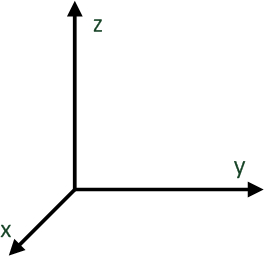
\includegraphics[width=\textwidth]{content/3_konzept/image/koordinatensystem_betrachter}
                \caption{Koordinatensystem des Betrachters \gls{g:worldframe}}
                \label{img:koord_betrachter}
        \end{subfigure}%
        \quad \quad
        \begin{subfigure}[htbp]{0.3\textwidth}
                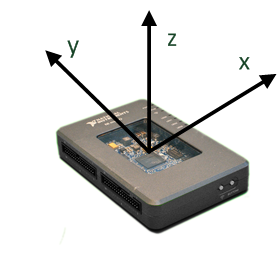
\includegraphics[width=\textwidth]{content/3_konzept/image/koordinatensystem_myRIO}
                \caption{Koordinatensystem \gls{g:myrio} \gls{g:bodyframe}}
                \label{img:koord_myRIO}
        \end{subfigure}        
        \caption{Koordinatensystem}\label{img:koordinatensystem}
\end{figure}    
%
Das \gls{g:myrio} hat bekanntlich eine beliebige Ausrichtung im Raum resp. im Koordinatensystem des Betrachters. Durch die Montage des Beschleunigungssensors sind dessen Achsen in Bezug auf das Geh�use gegeben. Diese sind in Abbildung \vref{img:koord_myRIO} ersichtlich.
%
\subsubsection*{Drehwinkel}
Der Drehwinkel $\phi$ wie in Abbildung \vref{img:Vektor} gesehen entspricht gerade dem Zwischenwinkel der beiden Vektoren $\overrightarrow{a\low{g}}$ sowie den \gls{ac:tp}-gefilterten Beschleunigungsdaten $\overrightarrow{a\low{grav}}$. Der Zwischenwinkel zweier Vektoren wird �ber das Skalarprodukt berechnet. Nach Papula \cite{lit:papula} ist dies wie in Gleichung \vref{eq:dotp} dargestellt m�glich.
%
\formula{
\overrightarrow{a\low{g}}*\overrightarrow{a\low{grav}} = \mid \overrightarrow{a\low{g}}\mid *\mid \overrightarrow{a\low{grav}}\mid *\cos(\phi)\\
\\
\phi=\arccos\left(\frac{\overrightarrow{a\low{g}}*\overrightarrow{a\low{grav}}}{ \mid \overrightarrow{a\low{g}}\mid *\mid \overrightarrow{a\low{grav}}\mid}\right)
}{
\phi & Zwischenwinkel der beiden Vektoren\\
\overrightarrow{a\low{g}} & Gravit�tsvektor\\
\overrightarrow{a\low{grav}} & gemessene Erdbeschleunigung
}[eq:dotp]
%
\subsubsection*{Rotationsachse}
Die Rotationsachse ben�tigt man, um eine Bezugsachse f�r die Drehung des Koordinatensystems des Sensors in das Koordinatensystems des Betrachters vorzunehmen. Die Rotationsachse muss somit senkrecht auf dem von den beiden bekannten Vektoren, dem Gravit�tsvektor $\overrightarrow{a\low{g}}$ und dem vom Beschleunigungssensor aufgenommenem Vektor $\overrightarrow{a\low{grav}}$ in welchem die Erdbeschleunigung auf die verschiedenen Komponenten verteilt ist, stehen. Dazu dient das Vektorprodukt, auch Kreuzprodukt genannt als Hilfsmittel. Das Vektorprodukt zweier Vektoren berechnet den Vektor, welcher senkrecht auf die von den beiden Vektoren aufgespannten Ebene steht. Die L�nge auch Norm oder Betrag dieses Vektors entspricht der von den beiden Vektoren aufgespannten Fl�che sowie nat�rlich der L�nge des Vektors. Wird der erhaltene Vektor zus�tzlich normiert, so hat dieser die L�nge Eins. Die Rotationsachse $\overrightarrow{n}$ wird wie in Gleichung \ref{eq:cross} berechnet.
%
\formula{
\overrightarrow{n} = \frac{\overrightarrow{a\low{g}} \times\overrightarrow{a\low{grav}}}{ \mid \overrightarrow{a\low{g}} \times \overrightarrow{a\low{grav}}\mid}
}{
\overrightarrow{n} & Richtung der Rotationsachse\\
\overrightarrow{a\low{g}} & Gravit�tsvektor\\
\overrightarrow{a\low{grav}} & gemessene Erdbeschleunigung
}[eq:cross]
%
% Verz�gerung
%\subsection{Berechnung der Bewegungsbeschleunigung} \todo{anpassen, Verz�gerung erw�hnen beschreiben}

%%
%Jede Filterung hat eine Verz�gerung des Signals zur Folge. Diese Verz�gerung verh�lt sich nach den Notizen in der Vorlesung Digitale Signalverarbeitung (BTE5034 DIGSV) bei Herrn Rolf Vetter wie in Gleichung \vref{eq:delay} aufgezeigt.
%%
%\formula{
%n_{d} = \frac{n_{b}}{2}
%}{
%n_{d} & Verz�gerung in Samples\\
%n_{b} & Anzahl Filterkoeffizienten
%}[eq:delay]
%
% Subtraktion
%\subsubsection*{Verz�gerung und Subtraktion}
%Die durch die Tiefpass-Filterung berechnete Erdbeschleunigung kann nicht direkt von der gemessenen Beschleunigung am Sensor abgezogen werden. Dies aus dem vorhin beschriebene Grund, dass jede Filterung eine Verz�gerung des Signals bewirkt. Die gemessene Beschleunigung am Sensor muss also zuerst um die zuvor berechnete Anzahl Samples aufgrund der Anzahl Filterkoeffizienten verz�gert werden. Dies kann man mit einem einfachen Verz�gerungselement erreichen. Die Funktion eines solchen Elementes ist in Abbildung \vref{img:delay} dargestellt.\par
%%
%% Verz�gerungselement
%\image{content/3_konzept/image/Verzoegerungselement}{scale=1}{htbp}[Verz�gerungselement][img:delay]
%%
%Nachdem das gemessene Signal zus�tzlich verz�gert wurde, kann das gefilterte Signal mit der beinhaltenden Erdbeschleunigungskomponente nun vom verz�gerten Signal abgezogen werden um die Beschleunigung der Bewegung zu erhalten.
%
% Hochpassfilterung
%\subsubsection*{Hochpassfilterung}
%Ein weiterer Ansatz ist, dass die gemessenen Daten mit einem Hochpass gefiltert werden. Die Beschleunigungskomponenten der Bewegung k�nnen somit von der als DC-Komponente auftretenden Erdbeschleunigung getrennt werden. Dabei ist zu beachten, dass die Filterl�nge des Tiefpassfilters und des Hochpassfilters gleich lang ist. Dies aus demselben oben genannten Grund, dass jede Filterung eine Verz�gerung des gefilterten Signals zur Ursache hat. Da die Erdbeschleunigung zur Kompensation der Orientierung verwendet wird und sp�ter wie im Abschnitt \vref{sub:rot} gezeigt auf die Bewegungsbeschleunigung angewendet wird muss die Verz�gerung beider Signale gleich ausfallen.
%
% Rotation
\subsection{Rotation}\label{sub:rot}
Um die Beschleunigung der Bewegung zu erhalten, k�nnen mehrere Ans�tze verfolgt werden. Ein Ansatz ist auf die gemessenen Beschleunigungsdaten zus�tzlich eine Hochpassfilterung anzuwenden. Hiermit wird gerade das Gegenteil zur Tiefpassfilterung erreicht. Mit der Hochpassfilterung werden die Beschleunigungsdaten von der Erdbeschleunigung gekapselt. Die Komponenten der Bewegungsbeschleunigung k�nnen somit mit einem Hochpass mit tief angelegter Durchlassfrequenz ermittelt werden. Doch genau hier liegt eine Schwierigkeit. Die Durchlassfrequenz muss sehr tief angesetzt werden damit auch langsame Bewegungen beachtet werden. Somit wurde dieser Ansatz schnell verworfen.\par 
%
In dieser Arbeit beschr�nken sich die Autoren nur auf die Bewegung in einer Ebene. In diesem Falle ist es ausreichen nur eine Rotation in das Betrachtungssystem vorzunehmen. Anschliessend ist die Bewegung auf der x- und y-Achse auszuwerten. Auf der z-Achse ist nach der Rotation nur die Erdbeschleunigung vorhanden. Wird die Rotation richtig ausgef�hrt, so ist die Erdbeschleunigung somit von der Bewegungsbeschleunigung entkoppelt.\par
%
Die Rotation wird ben�tigt, um das Koordinatensystem des Sensors in das Koordinatensystem des Betrachters zu transformieren. Dabei steht die zuvor berechnete Rotationsachse $\overrightarrow{n}$, um welche das System gedreht wird sowie der ermittelte Drehwinkel $\phi$ zwischen den beiden Vektoren zur Verf�gung. Die Rotationsmatrix kann mit diesen Parametern nach der im Kapitel \vref{ch:grundlagen} im Abschnitt \vref{sub:rot} beschriebenen Vorgehen aufstellt werden.\par
%
Mit der Rotationsmatrix und der berechneten Beschleunigung der Bewegung kann die Transformation vom Koordinatensystem des Sensors \gls{g:bodyframe} ins Koordinatensystem des Betrachters \gls{g:worldframe} mit einer einfachen Multiplikation erfolgen.
%
\formula{
a_{world} = a_{body} * R_{g; O; \overrightarrow{n}; \phi}
}{
a_{world} & Beschleunigung im Bezugskoordinatensystem \gls{g:worldframe}\\
R_{g; O; \overrightarrow{n}; \phi} & Rotationsmatrix um Gerade g mit Richtung $\overrightarrow{n}$ um Winkel $\phi$\\
a_{body} & Beschleunigung im Koordinatensystem des Sensors \gls{g:bodyframe} 
}[eq:delay]
%
Die Wirkung dieser Rotation ist in Abbildung \vref{img:rotation_vektor} ersichtlich. Hier ist eine Messung des beliebig orientierten Sensors im ruhenden Zustand und dessen rotierter Vektor dargestellt. Die z-Achse beinhaltet die Erdbeschleunigung, die Beschleunigung der Bewegung ist auf der x- sowie der y-Achse auszuwerten. Die Orientierung des Beschleunigungssensors ist kompensiert.
% 
\image{content/3_konzept/image/Rotation_Vektor}{scale=0.7}{htbp}[Rotation der Beschleunigungsdaten][img:rotation_vektor]
%
% Bewegungsdetektion
\subsection{Bewegungsdetektion}
Da die Integration einer Aufsummierung entspricht kann durch einen kleinen Fehler in der Rotation resultierend durch einen Offset bereits ein grosser Drift entstehen. Ein L�sungsansatz ist dabei eine Bewegungsdetektion einzuf�hren. Die Integration wir nur durchgef�hrt, wenn sich der Sensor auch bewegt. Ein Hilfsmittel �ber die Variation eines Signals ist deren Varianz respektive Standardabweichung. Die Standardabweichung gibt uns Information �ber die Verteilung der Signalamplitude. Wird der Sensor in Ruhe gelassen, so �ndern sich die aufgenommene Amplitude nur gering (Rauschen des Sensors laut NI \unit[3.9]{$mg_{rms}}$). Dementsprechend ist die Standardabweichung klein. Wird der Sensor bewegt, so resultiert eine gr�ssere �nderung der Amplitude. Die Standardabweichung wird somit gr�sser.\par
%
Zu Beginn jeder Messung wird der Sensor f�r \unit[4]{s} in Ruhe gelassen. In dieser Zeit kann der Threshold mittels der Standardabweichung �ber diese Zeit bestimmt werden. Da in dieser Zeit �ber eine verh�ltnism�ssig grosse Zeitdauer gemessen wird ist die Standardabweichung geringer als mit der Methode wo ein Fenster �ber das Signal gefahren wird und in diesem Fenster die Standardabweichung bestimmt wird. Aus diesem Grund wird zur Berechnung des Thresholds noch zus�tzlich ein Vorfaktor zur Standardabweichung multipliziert. Somit ist der Threshold gr�sser als die Standardabweichung des Rauschen. Dies ist sicherlich eine etwas unelegante L�sung und k�nnte noch verbessert werden. Jedoch wurde mit dieser Methode eine schnelle und einfache L�sung erzielt.\par
%
\image{content/3_konzept/image/Bewegungsdetect}{scale=0.7}{htbp}[Bewegungsdetektion auf der y-Achse][img:bewegungdetect]
%
Die Standardabweichung wird �ber ein Fenster w der L�nge \unit[200]{Smaples} berechnet. Somit erh�lt man die in Abbildung \vref{img:bewegungdetect} im unteren subplot dargestellte Standardabweichung. �bersteigt die Standartabweichung den zuvor definierten Threshold, so wird mit der Integration begonnen. Wird der Threshold anschliessend unterschritten, so ist keine Bewegung mehr vorhanden und es wird nicht mehr integriert. 
%
% Integration
\subsection{Integration}
%
\image{content/3_konzept/image/Integration}{scale=0.7}{htbp}[Bewegung auf der y-Achse][img:bewegung_y_achse]
%
Um von der Beschleunigung auf die Position zu schliessen, kann die Beschleunigung bekannterweise durch zweimaliges integrieren nach der Zeit berechnet werden. Integriert man die Beschleunigung einmal, so erh�lt man die Geschwindigkeit.
%
\formula{
v(t) = \int a(t)dt + v_0 
}{
v & Geschwindigkeit [$m/s$]\\
v_{0} & Anfangsgeschwindigkeit [$m/s$]\\
a & Beschleunigung [$m/s^2$]
}[eq:geschw]
%
Integriert man diese Geschwindigkeit erneut, so erh�lt man den zur�ckgelegten Weg �ber die betrachtete Zeitdauer.
%
\formula{
s(t) = \int v(t)dt + s_0 
}{
s & zur�ckgelegter Weg [m]\\
s_{0} & Anfangsposition [m]\\
v & Geschwindigkeit [$m/s$]
}[eq:weg]
% 
Die Integration erfolgt wie bereits im Kapitel \vref{ch:grundlagen} im Abschnitt \vref{sec:numint} beschrieben nummerisch mittels der Trapezmethode.
% 
%
%Software
\section{LabVIEW Rohdaten aufzeichnen}\label{s:konzept:sw}
		F�r die Verifikation des Konzept m�ssen Rohdaten des Beschleunigungssensors aufgenommen und in \gls{g:matlab} eingespeist werden. Dazu muss eine \gls{g:labview}-\acrshort{ac:vi} erstellt werden, die Daten aufnehmen und in einem \gls{g:matlab}-kompatiblen Format speichern kann. Das fertigen Projektdaten \texttt{concept\_reametric} sind im Anhang \vref{s:anhang_labview} zu finden.\par 
		%
		Als Basis f�r die \acrshort{ac:vi} dient das Standardprojekt \textsf{myRIO Project}\footnote{Das Projekt kann im Startdialog von \gls{g:labview} 2013 angew�hlt werden} von \gls{g:labview}, das folgende M�glichkeiten mitbringt:
		%
		\begin{itemize}
			\item Anbindung, inkl. Initialisierung den \gls{g:myrio}s
			\item Darstellung von aktuellen Beschleunigungsdaten in Diagramm
			\item Start und Stopp der Messung
		\end{itemize}
		%
		Damit die dargestellten Daten aufgezeichnet werden k�nnen, muss das bestehende Projekt mit den Komponenten Datei anlegen, Daten buffern und Daten speichern erg�nzt werden. F�r diesen Zweck werden die drei Zust�nde der bestehenden Sequenz angepasst.
		%
		\subsubsection*{Initialisierungs-Zustand}
			In der Initialisierung muss eine Datei f�r das sp�tere Speichern der Rohdaten erstellt werden. Dazu wird der in Abbildung \vref{img:init_file} ersichtliche Ablauf verwendet. Der Dateiname kann mit Hilfe eines Eingabefeldes (siehe Abbildung \vref{img:init_file_indicator}) individuell angepasst werden, muss aber die Endung \texttt{*.xlsx} aufweisen. Der Pfad der angelegten Datei bezieht sich auf das Home-Directory des \texttt{lvuser}, einem lokalen Benutzer des \gls{ac:ni} Real Time Linux. Der endg�ltige Speicherpfad wird anschliessend im letzten Zustand (Schliessen-Zustand) ausgegeben.
			%
			\begin{figure}[htbp] %htbp
				\centering
				\begin{subfigure}[b]{0.49\textwidth}
					\centering
					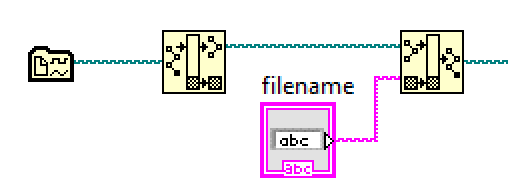
\includegraphics[scale=1]{content/3_konzept/image/init_file}  
					\caption{Blockdiagramm}
					\label{img:init_file}          
				\end{subfigure}
				\begin{subfigure}[b]{0.49\textwidth}
					\centering
					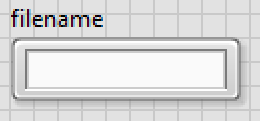
\includegraphics[scale=1]{content/3_konzept/image/init_file_indicator}  
					\caption{Frontpanel} 
					\label{img:init_file_indicator}         
				\end{subfigure}
				\caption{Datei erstellen}
				\label{img:datei_erstellen}
	    	\end{figure}\par
	    	%
	    	F�r das einfachere Einstellen der Sampling-Rate wird die Initialisierung noch durch eine solche M�glichkeit erg�nzt. F�r eine einfachere Interpretation wird zudem noch eine Umrechnung in Herz vorgenommen und angezeigt. Der Ablauf und das UI ist in der Abbildung \vref{img:periode} ersichtlich.
	    	%
			\begin{figure}[htbp] %htbp
				\centering
				\begin{subfigure}[b]{0.49\textwidth}
					\centering
					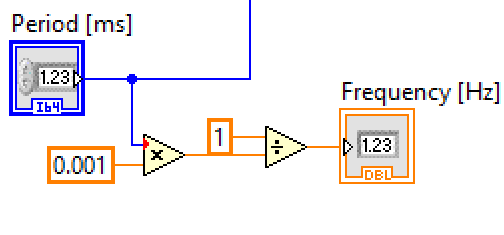
\includegraphics[scale=1]{content/3_konzept/image/init_periode}  
					\caption{Blockdiagramm}
					\label{img:init_periode}          
				\end{subfigure}
				\begin{subfigure}[b]{0.49\textwidth}
					\centering
					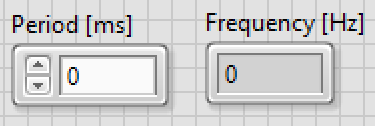
\includegraphics[scale=1]{content/3_konzept/image/init_periode_indicator}  
					\caption{Frontpanel} 
					\label{img:init_periode_indicator}         
				\end{subfigure}
				\caption{Sampling-Rate einstellen}
				\label{img:periode}
	    	\end{figure}
	    	%	
		%
		\subsubsection*{Datenaufzeichnen und Verarbeiten-Zustand}
			Der Hauptzustand dieses \gls{ac:vi}s besteht aus zwei Teilen. Der erste Teil beinhaltet einen Endlosschlaufe\footnote{genauer ein Time Loop, der eine genaue zyklische Ausf�hrung gew�hrleistet}, die zyklisch Beschleunigungsdaten und Timestamps einliest und buffert. Zus�tzlich werden die aktuellen Daten in Diagramm auf dem Frontpanel ausgegeben. Wird die Endlosschleife durch eine Fehler oder durch Bet�tigung der Stopp-Schaltfl�che beendet, so werden im zweiten Teil die gebufferten Daten mit Labels versehen, zu einer N x 4 Matrix zusammen gefasst und in eine Excel-Tabelle geschrieben. Dargestellt ist dieser Ablauf in der Abbildung \vref{img:process}. Die f�r die Bedienung erforderliche Komponenten k�nnen der Abbildung \vref{img:process_indicator} entnommen werden.
			%
			\begin{figure}[htbp] %htbp
				\centering
				\begin{subfigure}[b]{\textwidth}
					\centering
					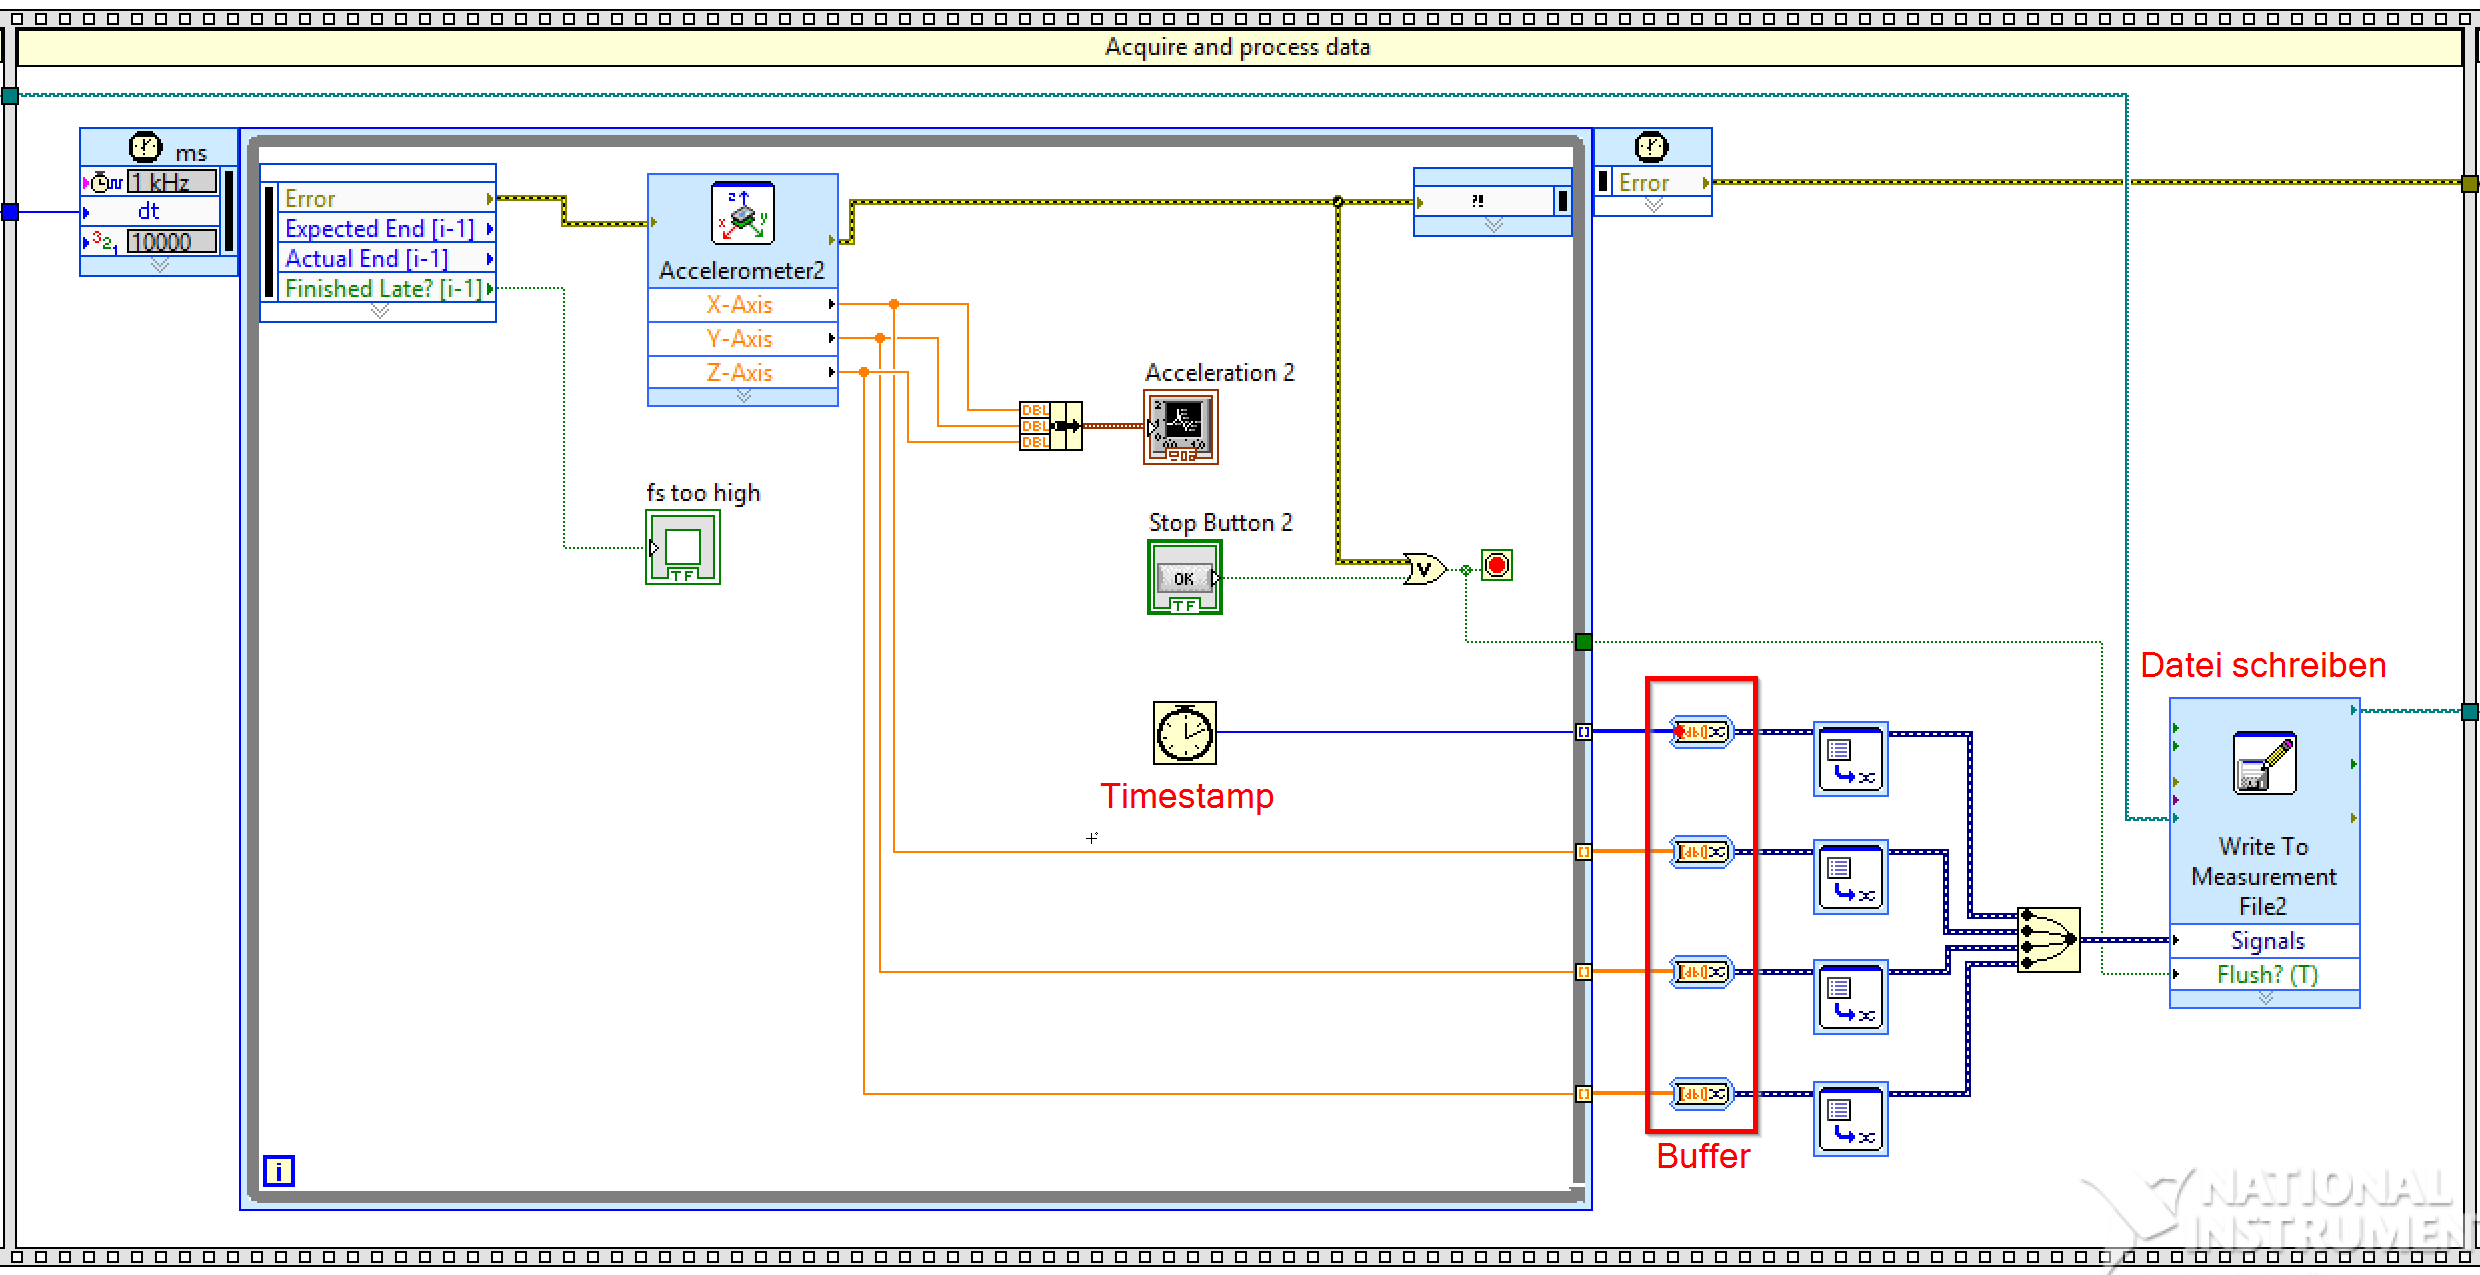
\includegraphics[scale=0.4]{content/3_konzept/image/process}  
					\caption{Blockdiagramm}
					\label{img:process}          
				\end{subfigure}
				\begin{subfigure}[b]{\textwidth}
					\centering
					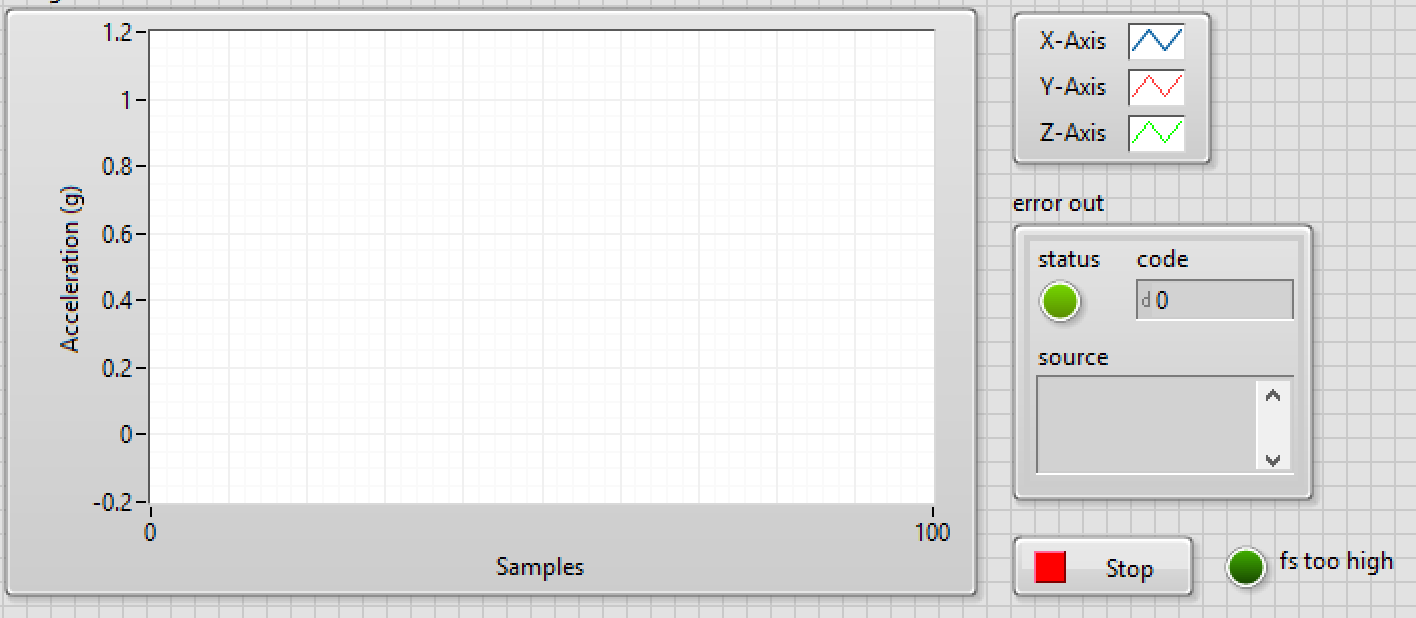
\includegraphics[scale=0.7]{content/3_konzept/image/process_indicator}  
					\caption{Frontpanel} 
					\label{img:process_indicator}         
				\end{subfigure}
				\caption{Daten einlesen und speichern}
				\label{img:daten_einlesen}
	    	\end{figure}
	    	%	
		%
		\subsubsection*{Schliessen-Zustand}
			Abgeschlossen wird das \gls{ac:vi} durch den Schliessen-Zustand. Dabei wird das \gls{g:myrio} auf den Ursprung zur�ckgesetzt und der Speicherpfad der Daten ausgeben. F�r diesen Zweck wird eine vorgefertigte \gls{ac:vi} von \gls{ac:ni} verwendet, die das Reseten des \gls{g:myrio}s durchf�hrt. Die Ausgabe des Pfades erfolgt bereits im vorderen Zustand, wird jedoch erst hier visualisiert. F�r das Blockdiagramm und das UI sei auf die Abbildung \vref{img:speicherpfad} verwiesen.
			%
			\begin{figure}[htbp] %htbp
				\centering
				\begin{subfigure}[b]{0.49\textwidth}
					\centering
					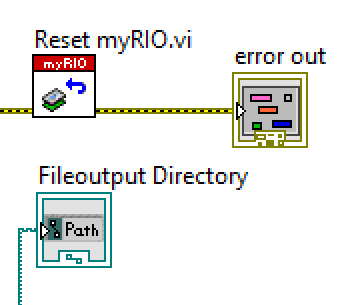
\includegraphics[scale=1]{content/3_konzept/image/close}  
					\caption{Blockdiagramm}
					\label{img:process}          
				\end{subfigure}
				\begin{subfigure}[b]{0.49\textwidth}
					\centering
					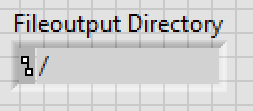
\includegraphics[scale=1]{content/3_konzept/image/close_indicator}  
					\caption{Frontpanel} 
					\label{img:close_indicator}         
				\end{subfigure}
				\caption{Speicherpfad angeben und \gls{g:myrio} reseten}
				\label{img:speicherpfad}
	    	\end{figure}\par
	    	%	
	%
	%\subsection{myRIO Posture Estimation}\label{subsec:myposture} \todo{gut darauf eingehen}
%
%
%Verifikation Rotation
\section{Verifikation Sch�tzung Rotationswinkel und Rotation}\label{s:verifikation_rotation}
	%
	%
	\subsection{Grund/Zweck der Messung}
		Die Sch�tzung des Rotationswinkels ist der erste Teil des Konzepts\footnote{siehe Abschnitt \vref{s:blockdiagramm}} und das erste von drei Experimental-Protokollen\footnote{die �brigen Protokolle sind in den Abschnitten \vref{s:verifikation_translation} und \vref{s:verifikation_transaltion_rotation} zu finden. Sie dienen als Ausgangslage f�r die Validierung des Konzepts.}. Sie dient als Basis f�r die sp�tere Rotation und anschliessende doppelte Integration und ist Voraussetzung f�r eine korrekte Messung. Die Winkel werden dabei hinsichtlich des Bezugssystems bestimmt. Das Protokoll soll die Genauigkeit des Algorithmus bestimmen und abw�gen ob sie den Anforderungen der Hypothese \vref{hypo:rotation} gen�gt.
		%
		\begin{hypo}\label{hypo:rotation}	   
			Der eingestellte Winkel wird durch die Sch�tzung richtig bestimmt.	
			Nach einer einmaligen Rotation haben die Komponenten x und y den Wert \unitfrac[0]{m}{s\high{2}} und die z-Komponente \unitfrac[9.81]{m}{s\high{2}}. Die Abweichung ist dabei nicht gr�sser als \unitfrac[0.01]{m}{s\high{2}}.
		\end{hypo}
	%
	%
	\subsection{Material/Testumgebung}
		Die Messung, respektive Sch�tzung der Rotationswinkel erfolgt statisch auf einer eigens f�r dieses Projekt entworfenen Testumgebung, die sp�ter zur Simulation eines Bewegungsablaufs des Knies gebraucht wird. Dazu siehe den Abschnitt \vref{ss:testumgebung_tran_rot}, indem auch n�her auf die M�glichkeiten des Aufbaus eingegangen wird. F�r dieses Protokoll wird lediglich von der Tatsache gebraucht gemacht, dass das \gls{g:myrio} kontrolliert in verschiedene Positionen gebracht und somit eine Reproduzierbarkeit der Messung gew�hrleistet werden kann.\par
		%
		F�r die Messung wird die Befestigung und der Bewegungsfreiraum des Testaufbaus so eingestellt, dass ein m�glichster grosser Winkelbereich zur Verf�gung steht (insgesamt \unit[56]{�})\footnote{Markierung XXX auf Schwenkarm}. Dazu wird der Rotationsarm sowie die Querverbindung wie in Abbildung  \vref{img:messaufbau_rot} gezeigt angeordnet. Die Position des \gls{g:myrio} M\low{1}, das f�r die Aufzeichnung der Beschleunigungsdaten eingesetzt wird, befindet sich am �ussersten Ende des Schwenkarm.\par
		%
		\image{content/3_konzept/image/aufbau_rot}{scale=1}{htbp}[Rotation - Testaufbau][img:messaufbau_rot]	
		%
		Die absolute Messung des eingestellten Winkels erfolgt �ber den Winkelmesser M\low{2}, der direkt am Schwenkarm befestigt ist (dazu siehe Abbildung \vref{img:messaufbau_tran_rot}). Alle verwendeten Messmittel sind in der Tabelle \vref{tab:messmittel_rot} aufgef�hrt und mit einer gesch�tzten Messgenauigkeit versehen.
		%
		\begin{table}[htbp]
     \centering
     \caption{Messmittelliste Verifikation Sch�tzung Rotationswinkel und Rotation}
     \label{tab:messmittel_rot}
     \begin{tabularx}{\textwidth}{|l|X|l|} 
         \hline
         \rowcolor{bfhblue}
         \textcolor{white}{Messmittel} & \textcolor{white}{Beschreibung} & \textcolor{white}{gesch�tzte Messgenauigkeit} \\
         \hline
         M\low{1} & \gls{g:myrio} 1900, Serial Number 03036833 & \unit[3.91]{mg} (\unit[1]{g} = \unitfrac[9.81]{m}{s\high{2}})\\
         \hline
         M\low{2} & JOHNSON Magnetic Angle Locator, NO. 700 & $\pm$\unit[1]{�}\\
         \hline
     \end{tabularx}  
\end{table}
	%
	%
	\subsection{Methoden}
		%
		\subsubsection*{Messgruppen}
			F�r die Messung werden zwei Messgruppen festgelegt. Die eine wird  als Testgruppe fungieren, wogegen die andere der Kontrolle dient.
			%
			\begin{itemize}
				%
				\item \textbf{Testgruppe} In der Testgruppe werden Beschleunigungsdaten durch das \gls{g:myrio} M\low{1} aufgezeichnet\footnote{siehe Abschnitt \vref{ss:rohdaten_aufzeichnen}} und gespeichert. Im Anschluss zur Messung werden die Daten in \gls{g:matlab} eingelesen und verarbeitet.
				%
				\item \textbf{Kontrollgruppe} Die zweite Gruppe repr�sentiert die direkte Messung mit Hilfe des Winkelmessers M\low{2}. Sie dient gleichzeitig der Kontrolle f�r die folgende Interpretation.
			\end{itemize}
			%
			Die unabh�ngige Variabel dieser Gruppen stellt die Messmethodik dar. 
		%
		\subsubsection*{Testgruppe Messmethodik}
			Die Messmethodik der Testgruppe basiert zum einen auf den aufgezeichneten Beschleunigungsdaten und zum anderen aus mathematischen Operationen\footnote{siehe Abschnitt \vref{s:blockdiagramm} f�r den verwendeten Algorithmus}, die die Winkelsch�tzung vornehmen. Zur Auswertung der Rotation dient das \gls{g:matlab}-Skript \texttt{XXX}, das im Anhang \vref{s:anhang_matlab} zu finden ist und auf dem ersten Teil des Konzept aufbaut. Im Konzept wird aus den in Ruhe aufgenommenen Beschleunigungsdaten die Rotationsmatrix berechnet. Mit dieser Rotationsmatrix gelingt die Transformation des \gls{g:bodyframe} in das \gls{g:worldframe}. Aus der aufgestellten Rotationsmatrix kann nach \cite{lit:craig} der pitch-Winkel wie in Gleichung \vref{eq:pitch} gezeigt berechnet werden. 
%
			\formula{
			M_{rot} &=\begin{bmatrix}a & b & c \\ d & e & f \\ g & h & i \end{bmatrix} \\[1ex]
			pitch &= atan2(-g,\sqrt{a^2 + d^2})
			}{
			M_{rot} & Rotationsmatrix\\
			pitch & Nick-Winkel
			}[eq:pitch]
%			
			Dieser pitch-Winkel entspricht gerade im Falle des in zuvor beschriebenem Testaufbau dem Nick-Winkel um welchen das \gls{g:myrio} um die im Abschnitt \vref{subsub:betrachter} definierte x-Achse gedreht wird. Somit wird der Winkel der Testgruppe aus der aufgestellten Rotationsmatrix aus dem Konzept berechnet.
		%
		\subsubsection*{Kontrollgruppe Messmethodik}
			Der Winkel der Kontrollgruppe wird direkt mit dem Winkelmesser M\low{2} gemessen. Zu beachten ist, dass dessen Winkelskala in \unit[90]{�} Bereiche unterteilt ist und deshalb ein gr�sserer Winkel durch Addition ermittelt werden muss. Als Referenz f�r die Auslenkung dient dabei die in Abbildung \vref{img:messaufbau_rot} ersichtliche \unit[0]{�}-Linie. Gemessen wird gegen den Uhrzeigersinn.
		%
		\subsubsection*{Testbeschreibungen}
			Es werden Messungen mit unterschiedlichen Rotationswinkel durchgef�hrt. Dazu wird der Testaufbau manuell in die gew�nschte Ausrichtung gebracht. Es wird zwischen f�nf verschiedenen Winkeln unterschieden, wie die Abbildung \vref{img:rot_winkeln} zeigt. Die Endwinkel (\unit[62]{�} und \unit[118]{�0} sind durch die mechanischen Einschr�nkungen bestimmt und stellen die maximale Auslenkung dar. Die Zwischenwinkel sind so gew�hlt, dass m�glichst gleichm�ssig der gesamte Bereich abgedeckt wird.\par
			%
			\image{content/3_konzept/image/rot_winkeln}{scale=0.4}{htbp}[Rotation-Winkeln][img:rot_winkeln]
			%
			Der Messablauf sieht folgende Schritte vor. Sie werden jeweils bei jedem Winkel wiederholt.
			\begin{enumerate}
				\item Testaufbau auf den gew�nschten Winkel einstellen. Dazu den Winkelmesser M\low{2} verwenden.
				\item \gls{g:labview}-Programm starten. Es m�ssen w�hrend  \unit[6]{s} Daten aufgezeichnet werden\footnote{Bedingt durch die Filterl�nge des Tiefpassfilters, siehe Abschnitt XXX}.
				\item den vorherigen Schritt 5-mal wiederholen.
				\item Datenextraktion nach mit den in Abschnitt \vref{ss:myRIO_hw} beschriebenen Methoden.
				\item Daten mit \gls{g:matlab} verarbeiten und auswerten.
			\end{enumerate}	
		%
		\subsubsection*{Datenauswertung}\todo{F�r alle Messungen separat std bestimmen; relativer Fehler kontrollieren!}
			Es gilt die Winkelsch�tzung hinsichtlich des eingestellten Winkels auszuwerten. Weiter muss die Rotation gepr�ft werden. Das Messergebnis der beiden Messgruppen stellt die abh�ngige Variabel dar.\par 
			%
			Die absolute Messabweichung, gemittelt\footnote{Es wird der arithmetische Mittelwert verwendet} �ber die f�nf Messungen,  betr�gt bei den unterschiedlichen Winkeln \unit[-2.28]{�} (\unit[62]{�}), \unit[-1.65]{�} (\unit[77]{�}), \unit[-1.45]{�} (\unit[90]{�}), \unit[-0.22]{�} (\unit[105]{�}) und \unit[0.74]{�} (\unit[118]{�}). Das entspricht einem mittleren absoluten Fehler von \unit[-0.92]{�} �ber alle Messungen hin betrachtet.\par
			%
			Der relative Messabweichungen, wiederum gemittelt, bemessen sich auf \unit[-0.038]{\%} (\unit[62]{�}), \unit[-0.021]{\%} (\unit[77]{�}), \unit[-0.016]{\%} (\unit[90]{�}), \unit[-0.002]{\%} (\unit[105]{�}) und \unit[0.006]{\%} (\unit[118]{�}). Dies ergibt einen mittleren relativen Fehler von \unit[-0.014]{\%} �ber alle Messungen hinweg.\par
			%
			Analysiert man die Messabweichung hinsichtlich ihrer Standardabweichung, so ergibt dies f�r die absoluten Messungen \unit[0.036]{�} und f�r die relativen \unit[0.0003]{\%}.\par 
			%
			Der Rotationswinkel kann zwar f�r eine Aussage �ber die Rotation verwendet werden, seine Bedeutung ist jedoch nur zweitrangig wenn die Rotation an sich nicht funktioniert. Daher gilt es die Beschleunigungskomponenten der einzelnen Achsen nach der Rotation auszuwerten. Bei allen Messungen ist der Beschleunigungsvektor $\overrightarrow{a}=[0\quad 0\quad 1]^{\top}$, was dem unbewegten Koordinatensystem des Betrachters entspricht (auf der z-Achse die Erdbeschleunigung).
			%
			Die Auswertung der Messungen zusammengefasst ist in der Tabelle \vref{tab:auswertung_tran} ersichtlich. 
			%
			\begin{table}[htbp]
     \centering
     \caption{Auswertung Messungen Rotation}
     \label{tab:auswertung_rot}
     \begin{tabularx}{\textwidth}{|X|r|r|r|r|} 
		\hline
		\rowcolor{bfhblue}
		\textcolor{white}{Messung} & \textcolor{white}{Absoluter Fehler} & \textcolor{white}{Relativer Fehler} & \textcolor{white}{Mittelwert}  & \textcolor{white}{Standardabweichung}\\
		\hline
		Rotation \unit[62]{�} & \unit[-2.28]{�} & \unit[-0.038]{\%} & \unit[59.72]{�} & \unit[0.009]{�}\\
		\hline
		Rotation \unit[77]{�} & \unit[-1.65]{�} & \unit[-0.021]{\%} & \unit[75.35]{�} & \unit[0.005]{�} \\
		\hline
		Rotation \unit[90]{�} & \unit[-1.45]{�} & \unit[-0.016]{\%} & \unit[88.55]{�} & \unit[0.009]{�}\\
		\hline
		Rotation \unit[105]{�} & \unit[-0.22]{�} & \unit[-0.002]{\%} & \unit[104.78]{�} & \unit[0.003]{�} \\
		\hline
		Rotation \unit[118]{�} & \unit[+0.74]{�} & \unit[+0.006]{\%} & \unit[118.74]{�} & \unit[0.152]{�} \\
		\hline
     \end{tabularx}  
\end{table}	 
			
	%
	%
	\subsection{Interpretation}\todo{Noch auf Messergebnisse Eingehen -> Sind sie plausibel?}
	Die zuvor definierte Hypothese \vref{hypo:rotation} ist best�tigt. Die vom \gls{g:bodyframe} ins \gls{g:worldframe} transformierten Beschleunigungskomponenten sind bei allen Messungen $\overrightarrow{a}=[0\quad 0\quad 1]^{\top}$. Also der Erdbeschleunigung auf der z-Achse.
%
%
%Verifikation Translation
\section{Verifikation Translation}\label{s:verifikation_translation}
	%
	%
	\subsection{Grund/Zweck der Messung}
		Die Verifikation der Translation stellt das zweite Experimental-Protokoll dar. Ziel der Messung ist es den kompletten Algorithmus hinsichtlich einer linearen Translation zu �berpr�fen. Dabei gilt es relevante Fakten wie Genauigkeit und Dynamik zu extrahieren und f�r die Validierung festzuhalten. Die in der Hypothese \vref{hypo:translation} festgelegten Anforderungen m�ssen erf�llt werden.
		%
		\begin{hypo}\label{hypo:translation}	    	
			Nach einer linearen Translation um die Distanz \unit[5]{cm} ist das Ergebnis des Algorithmus dieselbe. Die Abweichung ist dabei maximal $\pm$\unit[1]{cm}\footnote{Die Messgenauigkeit ist im Abschnitt \vref{ss:messgenauigkeit} erl�utert}. Die Position des \gls{g:myrio} hat keinen Einfluss auf das Messergebnis.
		\end{hypo}
	%
	%
	\subsection{Material/Testumgebung}\label{ss:material_translation}
		Die Messung muss reproduzierbar sein. Deshalb muss eine Testumgebung gew�hrleistet sein, die f�r eine Simulation einer geradlinigen Translation geeignet ist. Diese Voraussetzung erf�llt ein Kreuztisch einer Standbohr- / Fr�smaschine oder ein Werkzeugschlitten einer Drehbank. Damit k�nnen vorgegebene Pfade pr�zise in der x-y-Ebene gefahren werden.\par 
		%
		F�r die Messung wird der Werkzeugschlitten der Schaublin-Villeneuve M\low{3} aus der mechanischen Abteilung verwendet (siehe Abbildung \vref{img:drehbank}). Dieser erlaubt es eine kontrollierte Translation in der y-Richtung vorzunehmen. Weiter kommt als zentrale Komponente das \gls{g:myrio} M\low{1} zum Einsatz. Es dient der Aufzeichnung der Beschleunigungsdaten. Die gefahrene Distanz wird mit Hilfe des Massstabs M\low{3} angezeichnet\footnote{Der genau Vorschub kann der Bewegungsanforderung hinsichtlich der Geschwindigkeit nicht gerecht werden} (Abbildung \vref{img:distanz}).\par
		%
		\begin{figure}[htbp]
			\centering
			\begin{subfigure}[htbp]{0.7\textwidth}
			      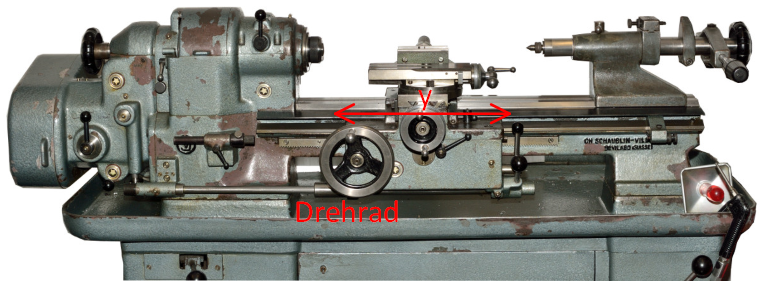
\includegraphics[height=3.5cm]{content/3_konzept/image/testaufbau_translation}
			      \caption{Drehbank}
			      \label{img:drehbank}
			      \vspace*{1.5ex}
			\end{subfigure}
			%
			\begin{subfigure}[htbp]{0.32\textwidth}
			      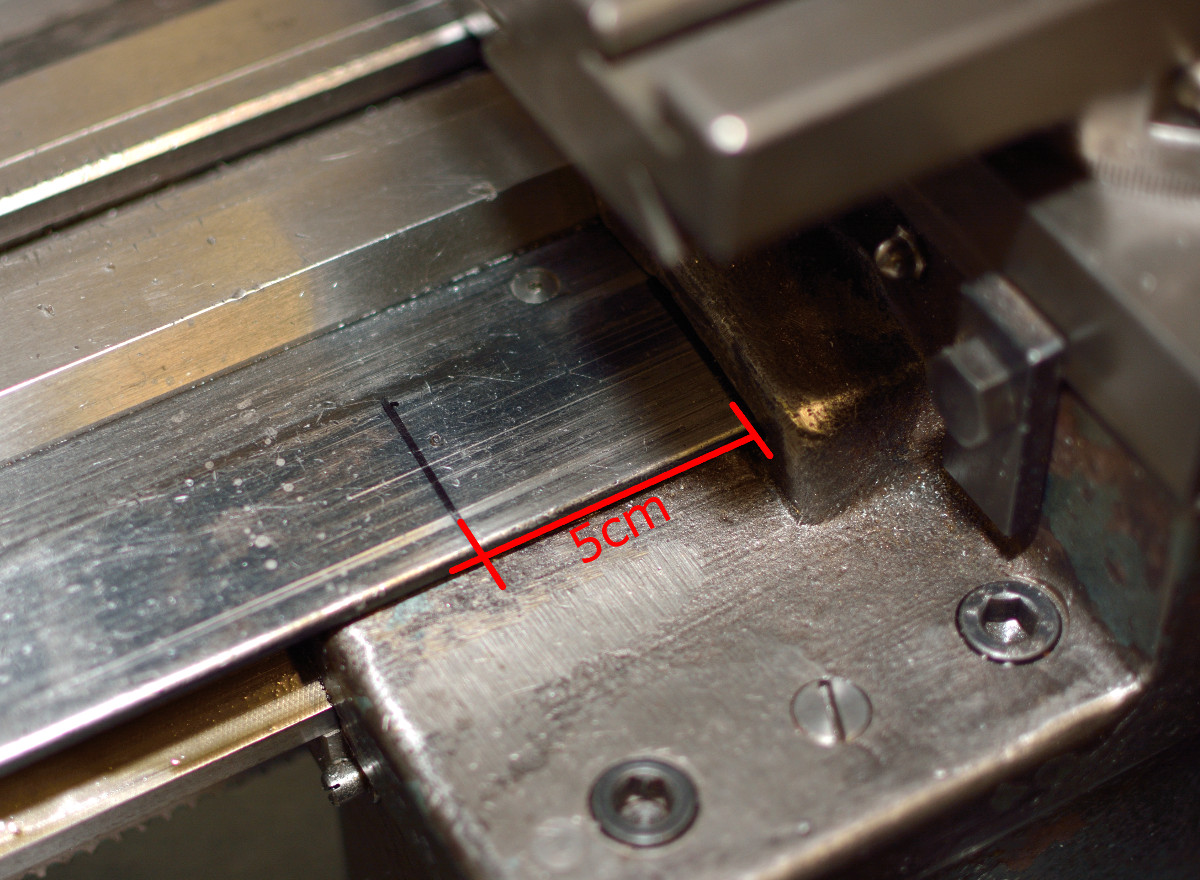
\includegraphics[height=3.5cm]{content/3_konzept/image/testaufbau_tran_distanz}
			      \caption{Translation-Distanz}
			      \label{img:distanz}
			\end{subfigure}        
			\caption{Translation - Testaufbau}
			\label{img:messaufbau_tran}
		\end{figure}    
		%
		Die Translation wird durch das Drehen des Drehrads ausgel�st. Die zur�ckgelegte Distanz wird dabei optisch durch den Bediener �berpr�ft (absolute Messung). Ein Setzen von mechanischen Anschl�ge w�rde das Messergebnis negativ beeinflussen, weshalb darauf verzichtet wird. Es wird zwischen zwei Translationsgeschwindigkeiten unterschieden, wobei die Geschwindigkeit durch die Bewegungszeit, gemessen mit der Stoppuhr M\low{4}, klassifiziert wird.\par
		%
		Das \gls{g:myrio} f�r die Messungen in unterschiedlichen Positionen am Werkzeugtisch angebracht. F�r die Befestigung dient ein Spannblock. Alle zum Einsatz gekommen Messmittel dieses Protokolls sind in der Tabelle \vref{tab:messmittel_translation} aufgelistet. Zudem ist eine gesch�tzte Genauigkeit angeben, die jedoch hinsichtlich der manuell durchgef�hrten Translation vernachl�ssigbar ist.
		%
		\begin{table}[htbp]
     \centering
     \caption{Messmittelliste}
     \label{tab:messmittel}
     \begin{tabularx}{\textwidth}{|l|X|l|} 
         \hline
         \rowcolor{bfhblue}
         \textcolor{white}{Messmittel} & \textcolor{white}{Beschreibung} & \textcolor{white}{gesch�tzte Messgenauigkeit} \\
         \hline
         M\low{1} & JOHNSON Magnetic Angle Locator, NO. 700 & $\pm$\unit[1]{�}\\
         \hline
         M\low{2} & \gls{g:myrio} 1900, Serial Number 03036833 & \unit[3.91]{mg} (\unit[1]{g} = \unitfrac[9.81]{m}{s\high{2}})\\
         \hline
     \end{tabularx}  
\end{table}
	%
	%
	\subsection{Methoden}
		%
		\subsubsection*{Messgruppen}
			Es werden zwei Messgruppen definiert. Die eine dient als Testgruppe und die andere als Kontrollgruppe. 
			%
			\begin{itemize}
				%
				\item \textbf{Testgruppe} Die Testgruppe repr�sentiert das \gls{g:myrio} M\low{1}, das zur Aufzeichnung der Beschleunigungsdaten ben�tigt wird. Dabei werden die Daten nur gespeichert und nicht verarbeitet\footnote{F�r detailliertere Informationen zur Aufzeichnung sei auf den Abschnitt \vref{ss:rohdaten_aufzeichnen} verwiesen}. Die Signalverarbeitung erfolgt zu einem sp�teren Zeitpunkt auf einem Computer mit Hilfe von \gls{g:matlab}.
				%
				\item \textbf{Kontrollgruppe} Die zweite Gruppe stellt die direkte Messung mit dem Werkzeugtisch dar. Sie ist gleichzeitig die Kontrollgruppe, die schlussendlich bei der Interpretation als Ausgangslage gilt.
			\end{itemize}
			%
			Die Messmethodik stellt bei den beschriebenen Gruppen die unabh�ngige Variabel dar.
		%
		\subsubsection*{Testgruppe Messmethodik}\label{ss:messmethodik_kontroll_tran}
			Die Translation wird indirekt durch die auftretenden Beschleunigungen gemessen. Dazu werden die aufgezeichneten Daten in das \gls{g:matlab}-Skript \textit{XXX} eingelesen, wo mit Hilfe von mathematischen Operationen die Distanz bestimmt wird. Das Skript ist im Anhang \vref{s:anhang_matlab} zu finden.
		%
		\subsubsection*{Kontrollgruppe Messmethodik}
			Die Aufnahme der Pfadl�nge erfolgt direkt mit dem Massstab M\low{2}. Die vergebene Distanz von \unit[5]{cm} wird dabei auf dem Schlitten der Drehbank M\low{3} vermerkt.
		%
		\subsubsection*{Testbeschreibungen}
			Es werden mehrere unterschiedliche Messungen, die sich hinsichtlich Geschwindigkeit und Positionierung unterscheiden, durchgef�hrt. Dazu wird das \gls{g:myrio} M\low{1} unterschiedlich positioniert. Um die Anzahl Messungen in eine �berschaubaren Rahmen zu halten, wird der Test auf 3 Positionen beschr�nkt. 
			%
			\begin{itemize}
				\item \textbf{x-Achse Position} Das \gls{g:myrio} M\low{1} wird flach auf dem Kreuztisch angebracht. Dabei zeigt die x-Achse des Beschleunigungssensors nach unten, sprich gleichgerichtet wie der Gravitationsvektor. Relative Beschleunigungen erfolgen in der x-y-Ebene in y-Richtung des Werkzeugtisches. Dies entspricht ebenfalls der y-Richtung (negativ) im Koordinatensystem des Betrachters, Abbildung \vref{img:koord_betrachter}. Eine schematische und reale Darstellung der Befestigung kann den Abbildungen \vref{img:x_achse} entnommen werden.
				%
				\begin{figure}[htbp]
					\centering
					\begin{subfigure}[htbp]{0.49\textwidth}
						\centering
					     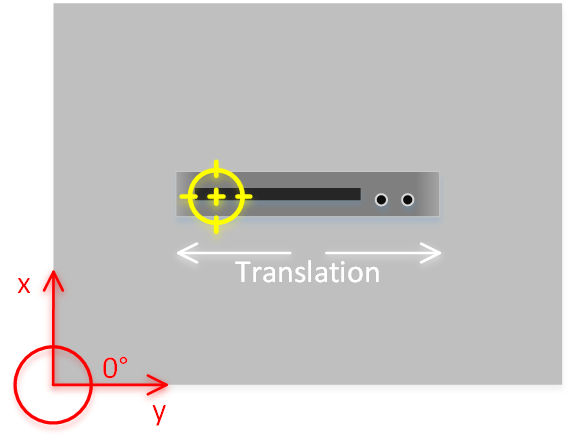
\includegraphics[height=3.7cm]{content/3_konzept/image/testaufbau_translation_position_x}
					     \caption{schematisch}
					     \label{img:x_schematisch}
					\end{subfigure}%
					\begin{subfigure}[htbp]{0.49\textwidth}
						\centering
					     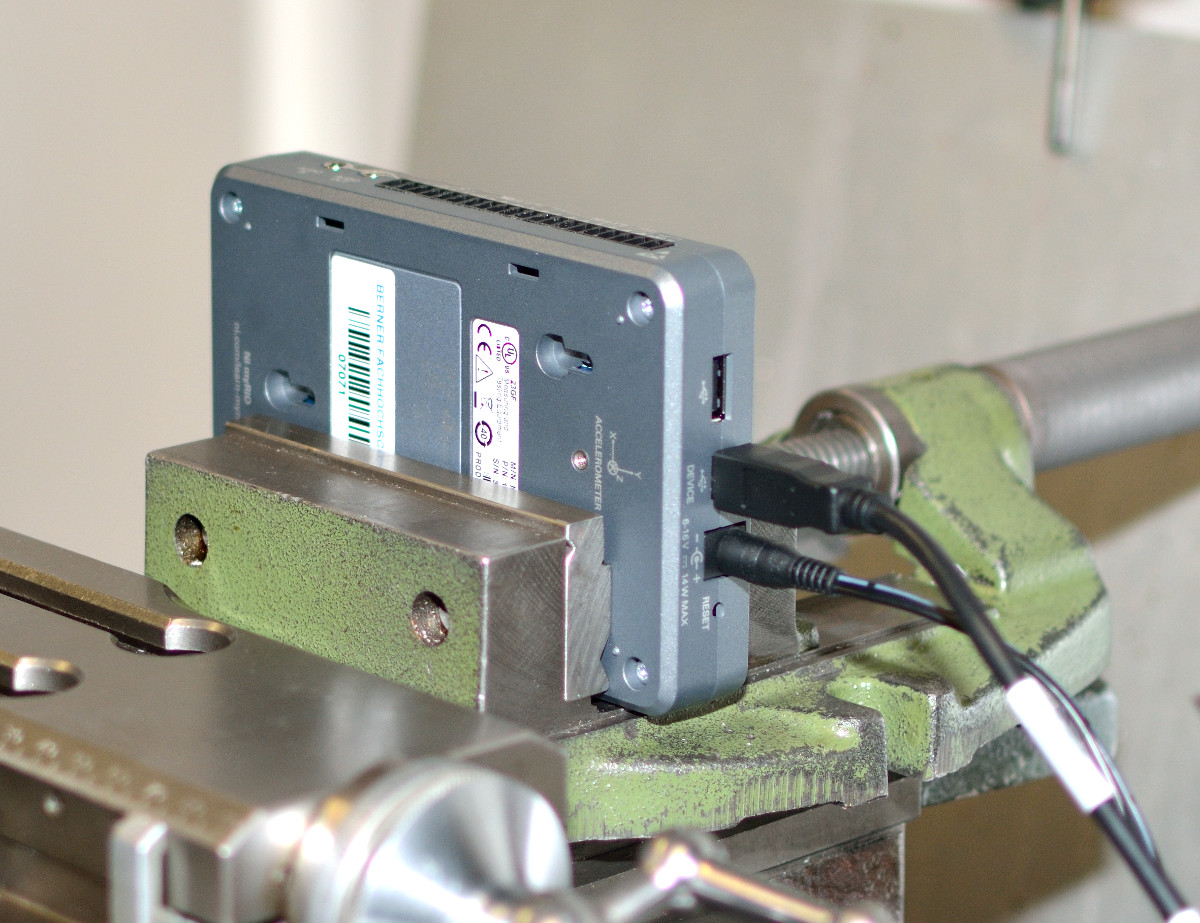
\includegraphics[height=3.7cm]{content/3_konzept/image/testaufbau_translation_position_x_real}
					     \caption{real}
					     \label{img:x_real}
					\end{subfigure}        
					\caption{x-Achsen Position}
					\label{img:x_achse}
				\end{figure}    
				%
				\item \textbf{y-Achse Position} Bei der zweiten Position wird das \gls{g:myrio} so angebracht, das die y-Achse des Beschleunigungssensors parallel zum Gravitationsvektor steht. Gemessene Beschleunigungen wirken sich somit nur auf die x- und z-Achse aus. Die Abbildung \vref{img:y_achse} verdeutlicht diesen Aufbau. Die Translation wird in der y-Achse (positiv) erfolgen, bezogen auf das Koordinatensystem des Betrachters.
				\begin{figure}[htbp]
					\centering
					\begin{subfigure}[htbp]{0.49\textwidth}
						\centering
						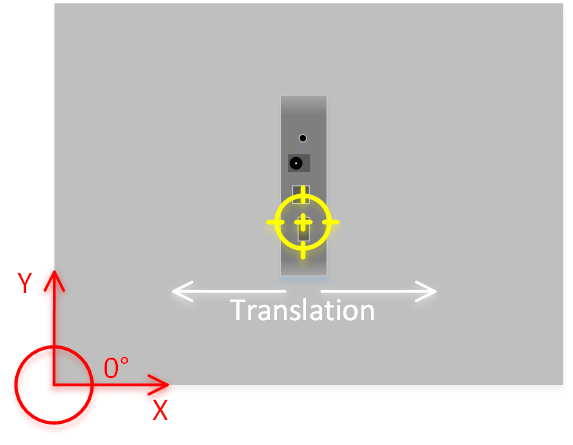
\includegraphics[height=3.7cm]{content/3_konzept/image/testaufbau_translation_position_y}
						\caption{schematisch}
						\label{img:y_schematisch}
					\end{subfigure}%
					\begin{subfigure}[htbp]{0.49\textwidth}
						\centering
						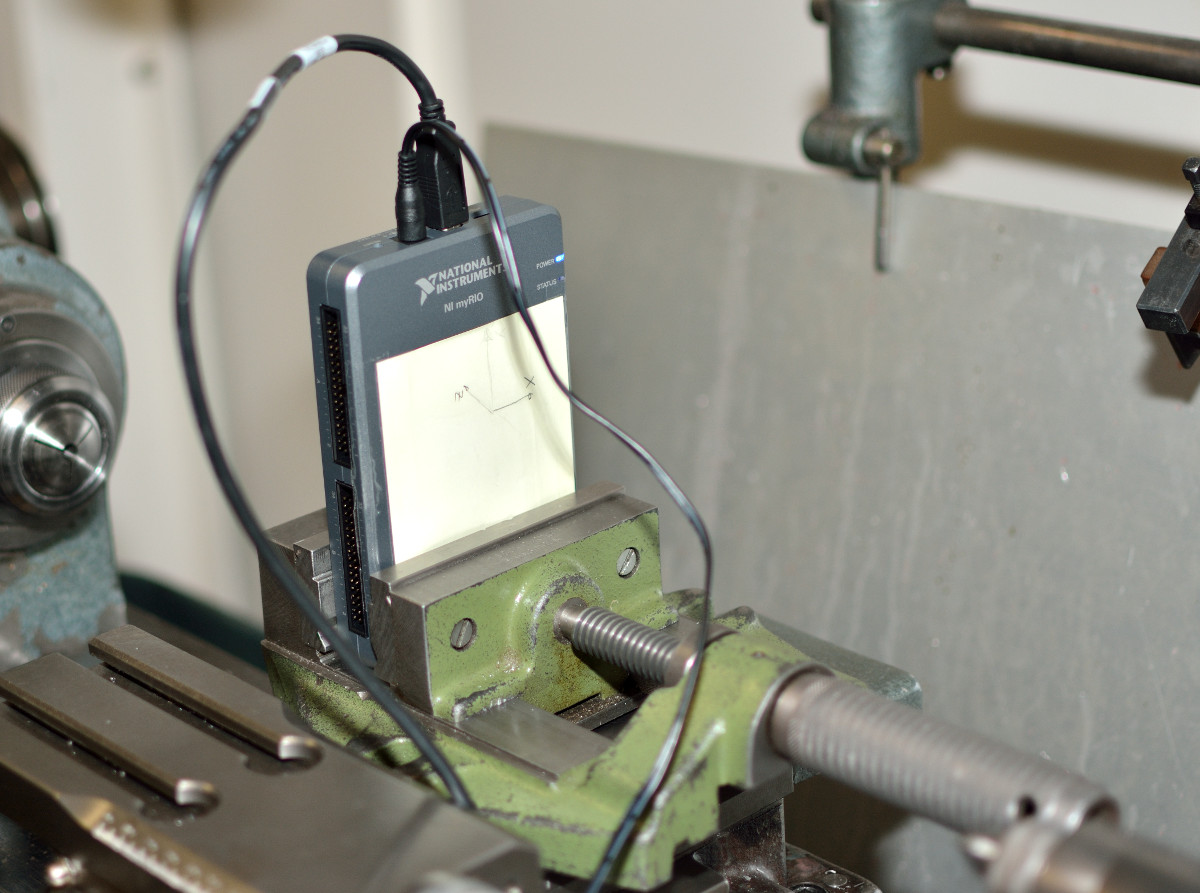
\includegraphics[height=3.7cm]{content/3_konzept/image/testaufbau_translation_position_y_real}
						\caption{real}
						\label{img:y_real}
					\end{subfigure}        
					\caption{y-Achsen Position}
					\label{img:y_achse}
				\end{figure}    
				%
				\item \textbf{z-Achse Position} Abschliessend erfolgt noch eine Positionierung mit der z-Achse des Beschleunigungssensors in Richtung des Gravitationsvektors (gleichgerichtet). Aus dieser Konstellation ergeben sich nur Beschleunigungen auf die x- und y-Achsen des Sensors, was eine negative Translation in negativer y-Richtung, bezogen auf das Koordinatensystem des Betrachters, zur Folge hat. Die Befestigungsrichtung des \gls{g:myrio}s M\low{1} ist in der Abbildung \vref{img:z_achse} zu sehen.
				\begin{figure}[htbp]
					\centering
					\begin{subfigure}[htbp]{0.49\textwidth}
						\centering
						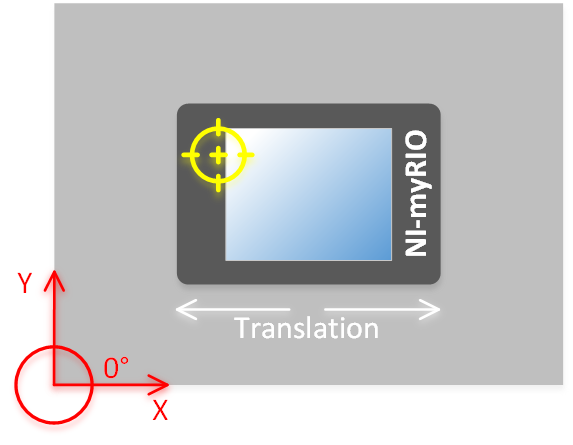
\includegraphics[height=3.7cm]{content/3_konzept/image/testaufbau_translation_position_z}
						\caption{schematisch}
						\label{img:z_schematisch}
					\end{subfigure}%
					\begin{subfigure}[htbp]{0.49\textwidth}
						\centering
						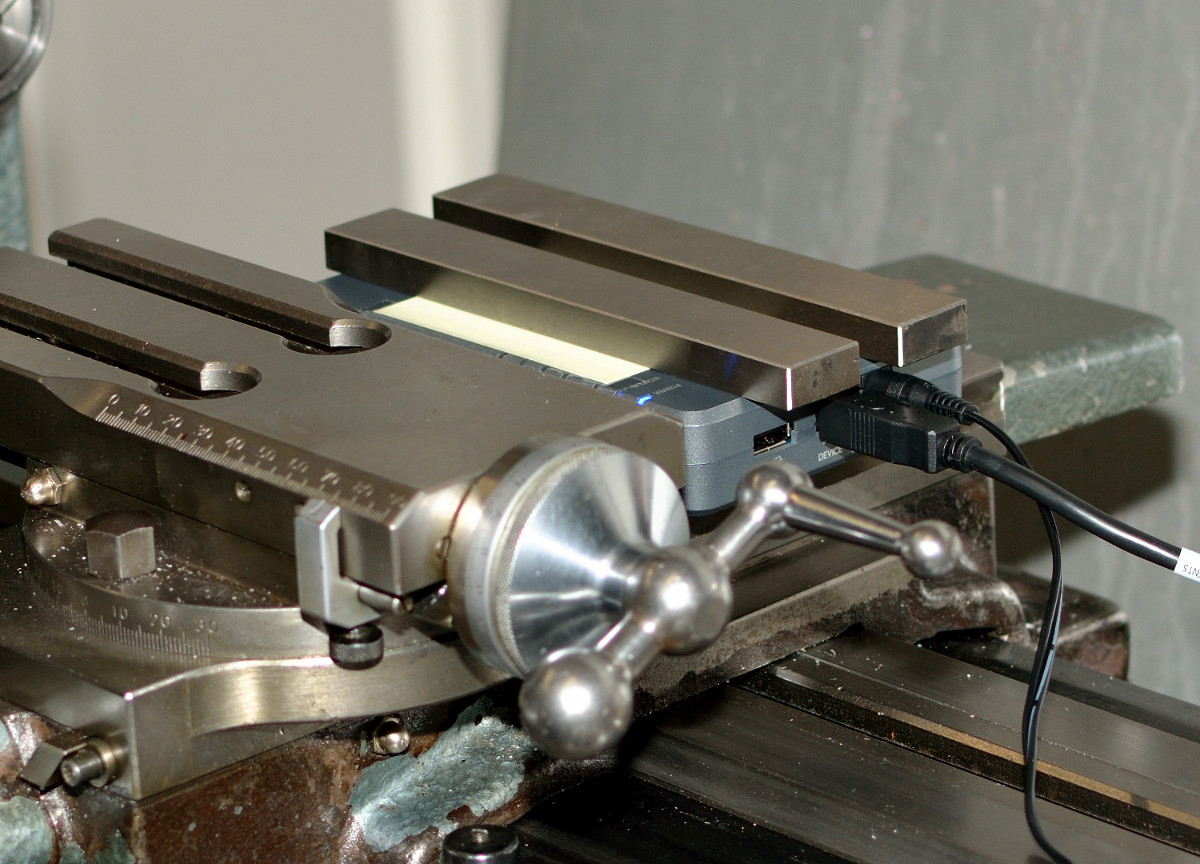
\includegraphics[height=3.7cm]{content/3_konzept/image/testaufbau_translation_position_z_real}
						\caption{real}
						\label{img:z_real}
					\end{subfigure}        
					\caption{z-Achsen Position}
					\label{img:z_achse}
				\end{figure}    
			\end{itemize}\par 
			%
			Die zu fahrende Distanz wird auf \unit[5]{cm} festgelegt. Dies entspricht dem  Messbereich, der in Abschnitt \vref{ss:messbereich} erl�utert ist. Bedingt durch die manuelle Durchf�hrung der Translation, kann eine Toleranz des zur�ckgelegten Pfades vorliegen. Diese ist innerhalb von $\pm$\unit[1]{cm} zu halten.\par
			%
			Wie im vorherigen Abschnitt \vref{ss:material_translation} er�rtert, wird die Geschwindigkeit in direkt �ber die Bewegungszeit gemessen. Daher werden lediglich zwei Bereiche definiert:
			\begin{itemize}
				\item \textbf{langsam} Die Translation dauert \unit[2]{s}. Diese Vorgabe wird nur rudiment�r mit einer Zeitmessung verifiziert (Stoppuhr M\low{4}).  
				%
				\item \textbf{schnell} Eine Bewegungszeit von \unit[1]{s}.
			\end{itemize}\par
			%
			Insgesamt ergeben sich durch die verschiedenen Positionierungen und Geschwindigkeiten 6 verschiedene Messungen. Der Messablauf gliedert sich in 5 Schritte. Alle Schritte sind bei jeder Positionierung und Geschwindigkeit 15 mal zu wiederholen. 
			%
			\begin{enumerate}
				\item Das \gls{g:myrio} M\low{1} wie vorgeben Positionieren.
				\item Den Werkzeugtisch an die markierte Startposition bewegen
				\item Das \gls{g:labview}-Programm starten.
				\item Messung starten
					\begin{enumerate}
						\item \unit[4]{s} warten bis die Rotationswinkel gesch�tzt sind.
						\item Translation durchf�hren (langsam oder schnell).
						\item Warten bis \unit[10]{s} verstrichen sind (totale Messzeit).
					\end{enumerate}
				\item Werkzeugtisch in Ursprungsposition bewegen.
			\end{enumerate}
		%
		\subsubsection*{Datenauswertung}
			Die relativ gemessene Distanz der Testgruppe muss bezogen auf die Kontrollgruppe ausgewertet werden. Die ermittelte Entfernung ist dabei die abh�ngige Variabel dieses Protokolls. Die Messresultate werden hinsichtlich der Messabweichung und ihrer Standardabweichung untersucht. F�r die Auswertung irrelevanten Diagramme sei auf den Anhang \vref{ss:anhang_konzept_messung_translation} verwiesen.\par
			%
			\paragraph*{x-Achsen Position}
				�ber 15 Messungen mit der langsamen Geschwindigkeit tritt ein mittlere absoluter Fehler von \unit[0.44]{cm} auf, was ein relativ \unit[8.8]{\%} ergibt. Die gemessenen Translationen, zu sehen in der Abbildung \vref{img:x_tran_langsam_y}, weissten eine mittlere Distanz von \unit[-4.56]{cm} (blaue Linie) mit einer Standardabweichung (rote Linien) von \unit[0.477]{cm} auf.
				\image{content/3_konzept/image/mittel_5_X_Y}{scale=0.6}{htbp}[x-Position Translation langsam][img:x_tran_langsam_y]
				%
				Wird die Geschwindigkeit verdoppelt auf Stufe schnell, so verbessert sich der mittlere absolute Fehler auf \unit[0.205]{cm}. Dies entspricht einer relativen Abweichung von \unit[4.1]{\%}. Daraus ergibt sich ein mittlere gemessene Distanz von \unit[-4.795]{cm} mit einer Standardabweichung von \unit[0.369]{cm}. Ersichtlich ist die Messung und die Auswertung in der Abbildung \vref{img:x_tran_schnell_y}.
				%
				\image{content/3_konzept/image/mittel_5_X_Y}{scale=0.6}{htbp}[x-Position Translation schnell][img:x_tran_schnell_y]
%				\begin{figure}[htbp]
%					\centering
%					\begin{subfigure}[htbp]{0.8\textwidth}
%						\centering
%						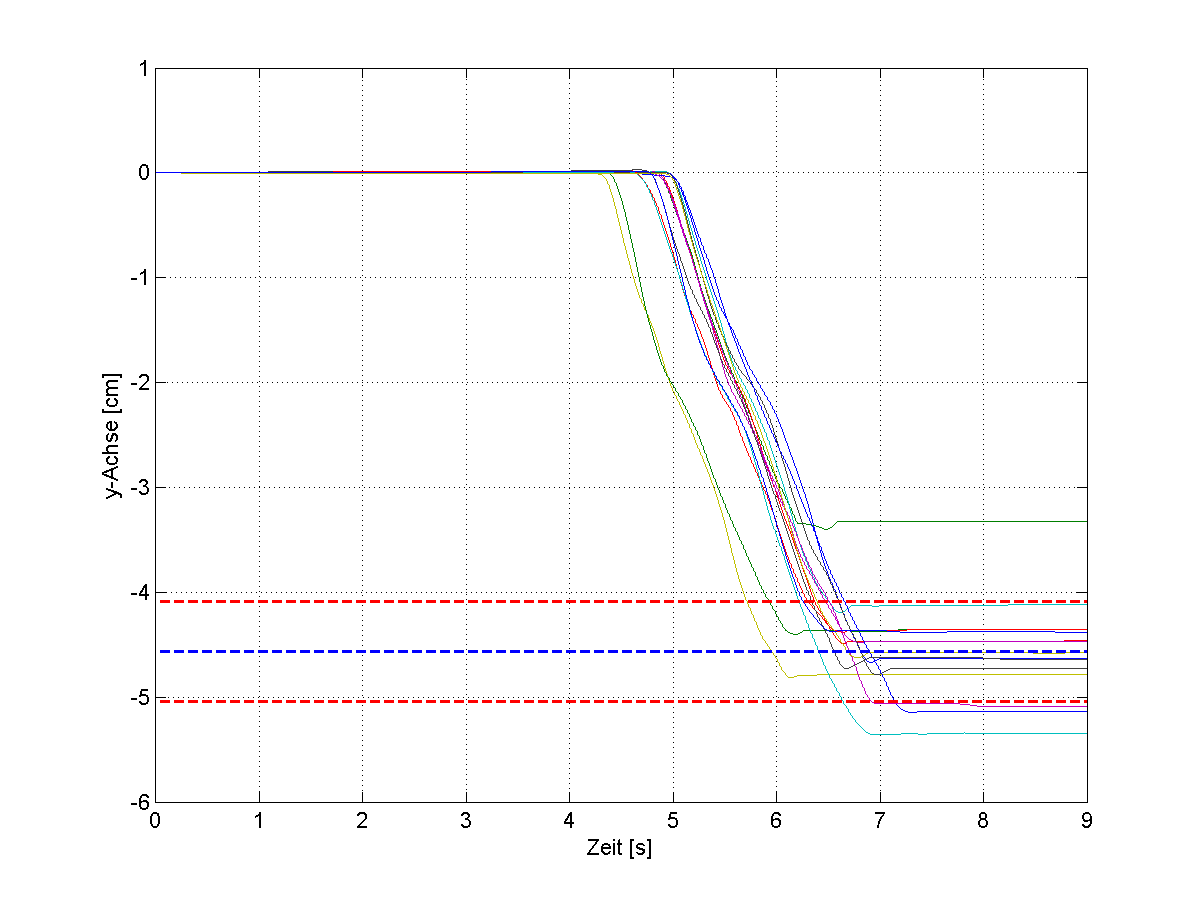
\includegraphics[height=8cm]{content/3_konzept/image/mittel_5_X_Y}
%						\caption{langsam}
%						\label{img:x_tran_langsam_y}
%						\vspace*{1.5ex}
%					\end{subfigure}\\
%					\begin{subfigure}[htbp]{0.8\textwidth}
%						\centering
%						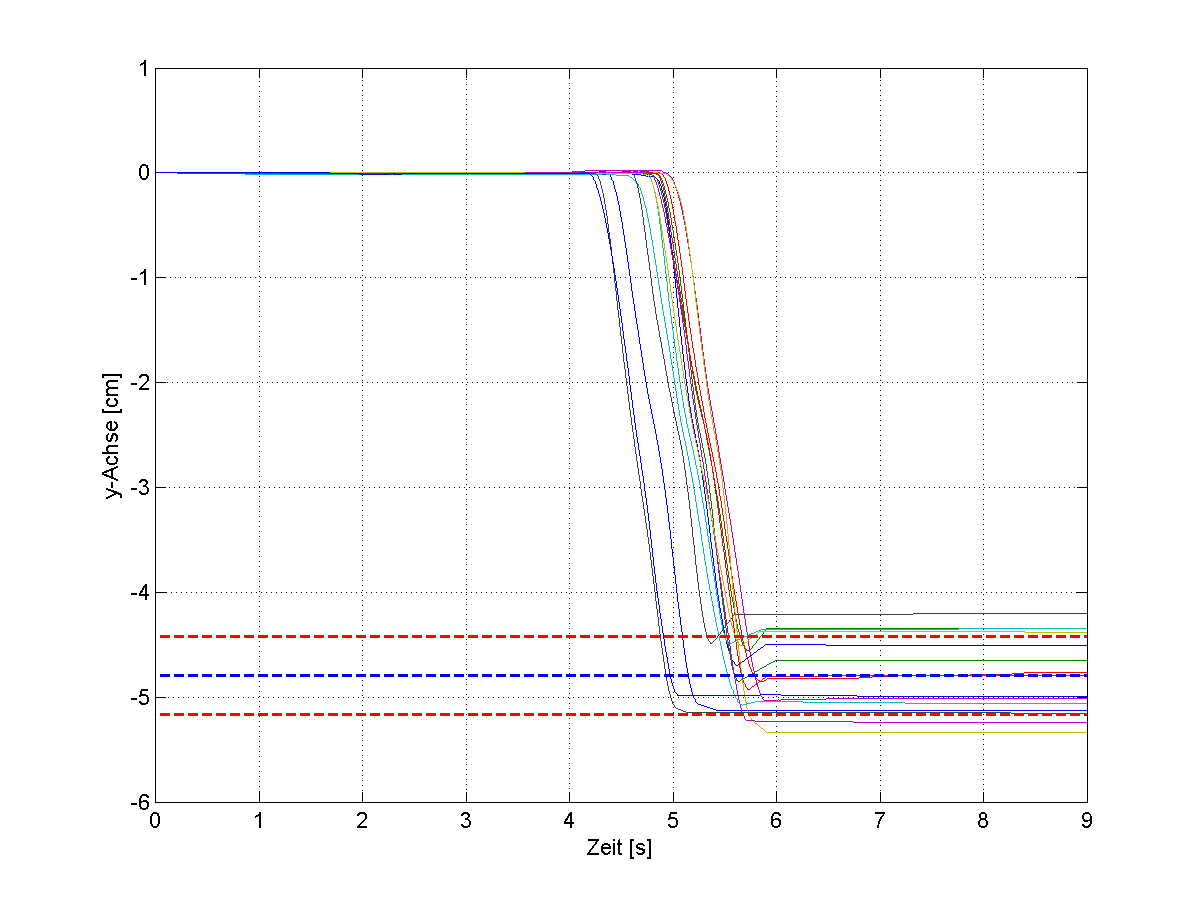
\includegraphics[height=8cm]{content/3_konzept/image/schnell_5_X_Y}
%						\caption{schnell}
%						\label{img:x_tran_schnell_y}
%					\end{subfigure}        
%					\caption{x-Position Translation y-Richtung}
%					\label{img:x_tran_schnell}
%				\end{figure}    
			%
			\paragraph*{y-Achsen Position}
				Befindet sich das \gls{g:myrio} in der y-Achsen Position, so ergibt sich �ber 15 Messungen ein mittlerer absoluter Fehler von \unit[1.338]{cm} (relativ \unit[26.8]{\%}). Dies bei der Geschwindigkeit langsam. Die Analyse hinsichtlich des gemessenen Mittelwertes und Standardabweichung ergibt \unit[6.338]{cm} und \unit[1.355]{cm}. Die Abbildung \vref{img:y_tran_langsam_y} zeigt die 15 Messungen mit eingezeichneten Kenngr�ssen (blau Mittelwert der Messung und rot die Standardabweichung).
				%
				\image{content/3_konzept/image/mittel_5_Y_Y}{scale=0.6}{htbp}[y-Position Translation langsam][img:y_tran_langsam_y]
				%
				Ein Erh�hung der Geschwindigkeit bringt einen mittleren absoluten Messfehler von \unit[1.360]{cm} und ein relativen von \unit[27.2]{\%} zu Tage. Dies bei einem ermittelten Mittelwert von \unit[6.360]{cm} und einer Standardabweichung von \unit[0.697]{cm}, wie die Abbildung \vref{img:y_tran_schnell_y}.
				%
				\image{content/3_konzept/image/schnell_5_Y_Y}{scale=0.6}{htbp}[y-Position Translation schnell][img:y_tran_schnell_y]
			%
			\paragraph*{z-Achsen Position}
				Die abschliessende Messung in der z-Achsen Position ergibt bei der langsamen Geschwindigkeit einen absoluten mittleren Fehler von \unit[2.043]{cm}, was einem relativen Fehler von \unit[40.9]{\%} entspricht. Betrachtet man die Abbildung \vref{img:z_tran_langsam_y}, so zeigt sich bei der blauen Linie ein Mittelwert von \unit[-2.957]{cm} bei einer Standardabweichung von \unit[0.323]{cm}.
				%
				\image{content/3_konzept/image/mittel_5_Z_Y}{scale=0.6}{htbp}[z-Position Translation y-Richtung langsam][img:z_tran_langsam_y]
				%
				Bei der Geschwindigkeit schnell erh�ht sich wiederum der absolute Fehler auf \unit[0.769]{cm} (entspricht relativ \unit[15.4]{\%}). Die Messung an sich hat einen Mittelwert von \unit[-4.231]{cm} bei einer Standardabweichung von \unit[0.255]{cm}. Die Abbildung \vref{img:z_tran_schnell_y} zeigt das gemessene Ergebnis.\par 
				%
				\image{content/3_konzept/image/schnell_5_Z_Y}{scale=0.6}{htbp}[z-Position Translation schnell][img:z_tran_schnell_y]
			%
			Die Messerergebnisse zusammengefasst sind in der Tabelle \vref{tab:auswertung_tran} dargestellt. Darauf basierend erfolgt nun im folgenden Abschnitt \vref{ss:interpretation_tran} die Interpretation und Diskussion.
			%
			\begin{table}[htbp]
     \centering
     \caption{Auswertung Messungen Translation}
     \label{tab:auswertung_tran}
     \begin{tabularx}{\textwidth}{|X|r|r|r|r|} 
		\hline
		\rowcolor{bfhblue}
		\textcolor{white}{Messung} & \textcolor{white}{Absoluter Fehler} & \textcolor{white}{Relativer Fehler} & \textcolor{white}{Mittelwert}  & \textcolor{white}{Standardabweichung}\\
		\hline
		x-Achsen Position langsam & \unit[0.34]{cm} & \unit[6.8]{\%} & \unit[-4.66]{cm} & \unit[0.35]{cm}\\
		\hline
		x-Achsen Position schnell & \unit[0.19]{cm} & \unit[3.8]{\%} & \unit[-4.81]{cm} & \unit[0.35]{cm} \\
		\hline
		y-Achsen Position langsam & \unit[2.20]{cm} & \unit[44.1]{\%} & \unit[7.20]{cm} & \unit[0.47]{cm}\\
		\hline
		y-Achsen Position schnell & \unit[1.34]{cm} & \unit[26.8]{\%} & \unit[6.34]{cm} & \unit[0.56]{cm} \\
		\hline
		z-Achsen Position langsam & \unit[2.20]{cm} & \unit[44.1]{\%} & \unit[-2.8]{cm} & \unit[0.36]{cm} \\
		\hline
		z-Achsen Position schnell & \unit[0.71]{cm} & \unit[14.1]{\%} & \unit[-4.29]{cm} & \unit[0.23]{cm}\\
		\hline
     \end{tabularx}  
\end{table}	 
	%
	%
	\subsection{Interpretation}\label{ss:interpretation_tran}\todo{Histogramm, Gruppenvergleich,Messfehler}
%
%
%Verifikation Translation und Rotation �berlagert
\section{Verifikation Translation und Rotation �berlagert}\label{s:verifikation_transaltion_rotation}
	%
	%
	\subsection{Grund/Zweck der Messung}\todo{anpassen an Abschnitt 3.1}
		Der Bewegungsablauf eines Knies umfasst eine Translation, die mit einer Rotation �berlagert ist. F�r eine abschliessende �berpr�fung des Algorithmus sollen nun diese beiden Komponenten zeitgleich �berpr�ft werden. Im Falle eines positiven Messergebnisse kann das Konzept, respektive der Algorithmus als geeignet betrachtet und implementiert werden. Die Anforderungen an das Messergebnis sind in der Hypothese \vref{hypo:tran_rot} festgelegt.
		\begin{hypo}\label{hypo:tran_rot}
			Das Messergebnis ist eine Bewegung in der \gls{g:transversalebene}, wobei nur die y-Komponente interessiert. Sie ist dabei eine Widerspiegelung des reale Ablaufs mit einer Abweichung von $\pm$\unit[1]{cm}\footnote{Erl�uterungen zur geforderten Messgenauigkeit sind im Abschnitt \vref{ss:messgenauigkeit} zu finden}.
		\end{hypo}
	%
	%
	\subsection{Material/Testumgebung}\label{ss:testumgebung_tran_rot}
		F�r eine aussagekr�ftige Messung muss eine Kniebewegung m�glichst exakt nachgebildet werden k�nnen. Weiter sollten die Messungen reproduzierbar sein. F�r diesen Zweck wurde eigens eine Mechanik konstruiert und aufgebaut.\par 
		%
		Der Simulator basiert auf Bosch-Profilen\footnote{Hergestellt von der Firma Bosch Rexroth AG: \url{http://www.boschrexroth.com}} und ist durch das sehr anpassbar. Der Aufbau erlaubt es einen vollst�ndigen statischen Bewegungsablauf nachzubilden, jedoch ohne die horizontal Rotation zu ber�cksichtigen. F�r eine konstante Geschwindigkeit des Ablaufs sorgt ein DC-Motor mit Rutschkupplung. Dieser wird mit einem DC-Netzteil gespiesen, was zugleich eine Steuerung der Geschwindigkeit erm�glicht (durch Variation der Spannung). Die Befestigung des \gls{g:myrio} M\low{1} erfolgt auf einer Platte, die wiederum auf dem Schwenkarm angebracht ist. Die Position ist dabei so gew�hlt, dass sie der Knieh�he eines Durchschnittsmensches entspricht. F�r das errechnen der Bewegungsbahn wird ausserdem ein Winkelmessger�t M\low{2} befestigt, das eine absolute Messung des Winkels erlaubt. Der komplette Aufbau ist in der Abbildung \vref{img:messaufbau_tran_rot} ersichtlich
		%
		\image{content/3_konzept/image/messaufbau_tran_rot}{scale=0.2}{htbp}[Messaufbau Translation, Rotation �berlagert][img:messaufbau_tran_rot]
		%
		Die Bedienung der Messeinrichtung kann auf zwei Arten erfolgen. Automatisch mit DC-Motor oder manuell von Hand (erm�glicht durch die Rutschkupplung). Im automatischen Betrieb kann die Geschwindigkeit, wie bereits zuvor erw�hnt, mit Variation der angelegten Spannung eingestellt werden. Der zul�ssige Spannungsbereich des Motors liegt dabei zwischen \unit[8]{V} und \unit[12]{V}. Wird die Bewegung manuell ausgel�st ist darauf zu achten, dass der Ablauf mit einer m�glichst konstanten Geschwindigkeit erfolgt. Um unterschiedliche Auslenkungen �berpr�fen zu k�nnen, kann die Querverbindung stufenlos am Rotationsarm verstellt werden\footnote{Markierung XXX, XXX und XXX am Rotationsarm}. Eine Auflistung aller verwendeter Messmittel, inklusive ihrer gesch�tzten Messgenauigkeit ist in der Tabelle \vref{tab:messmittel_tran_rot} vermerkt.
		%
		\begin{table}[htbp]
     \centering
     \caption{Messmittelliste Verifikation Translation und Rotation �berlagert}
     \label{tab:messmittel_tran_rot}
     \begin{tabularx}{\textwidth}{|l|X|l|} 
         \hline
         \rowcolor{bfhblue}
         \textcolor{white}{Messmittel} & \textcolor{white}{Beschreibung} & \textcolor{white}{gesch�tzte Messgenauigkeit} \\
         \hline
         M\low{1} & \gls{g:myrio} 1900, Serial Number 03036833 & \unit[3.91]{mg} (\unit[1]{g} = \unitfrac[9.81]{m}{s\high{2}})\\
         \hline
         M\low{2} & JOHNSON Magnetic Angle Locator, NO. 700 & $\pm$\unit[1]{�}\\
         \hline
         M\low{3} & THURLBY THANDAR INSTRUMENTS PL320 32V-2A PSU, Inv.-Nr. 190.0111 & \unit[0.1]{V}\\
         \hline
         M\low{4} & KDS Massstab \unit[50]{cm}, 60.3.12 & \unit[200]{$\mu$m}\\
         \hline
     \end{tabularx}  
\end{table}	
	%
	%
	\subsection{Methoden}
		%
		\subsubsection*{Messgruppen}\label{sss:messgruppe_tran_rot}
			Die Messung wird mit zwei Messgruppen durchgef�hrt, wobei die eine als Testgruppe und die andere als Kontrollgruppe verwendet wird.	
			%
			\begin{itemize}
				%
				\item \textbf{Testgruppe} Die Testgruppe beinhaltet das \gls{g:myrio} M\low{1} mit integriertem Beschleunigungssensor. Die Daten werden w�hrend des Tests aufgezeichnet und sp�ter auf dem Computer mit \gls{g:matlab} verarbeitet. 
				%
				\item \textbf{Kontrollgruppe} Die Kontrollgruppe dient als Basis f�r die sp�tere Auswertung. Die Aufnahme der Daten erfolgt zum einen Messtechnisch (Radius und Winkel) und zum anderen mathematisch (Berechnung der Pfadl�nge).
			\end{itemize}
			%
			Das unterschiedliche Messverfahren stellt die unabh�ngige Variabel in diesem Protokoll dar.
		%
		\subsubsection*{Testgruppe Messmethodik}
			Die Messmethodik der Testgruppe ist �quivalent zur Messmethodik des vorherigen Protokolls im Abschnitt \vref{ss:messmethodik_kontroll_tran}. F�r die bessere Gliederung der Protokolle wurde dennoch eigens das \gls{g:matlab}-Skript \texttt{XXX} erstellt. F�r eine detaillierte Einsicht ins Skript sei auf den Anhang \vref{s:anhang_matlab} verwiesen.
		%
		\subsubsection*{Kontrollgruppe Messmethodik}
			Wie abget�nt verwendet die Kontrollgruppe messtechnische und mathematische Verfahren um den zur�ckgelegte Weg zu ermitteln.  
			Gemessen wird mit Hilfe von Massstab M\low{4} und Winkelmesser M\low{2} die aktuelle Knieh�he (konstant �ber alle Messungen hinweg) und der m�gliche Winkelbereich $\alpha$ der aktuellen Auslenkung. Als Ausgangslage f�r die Aufnahme der skalaren Messgr�ssen dient die Abbildung \vref{img:messaufbau_dimensionen}. 
			%
			\image{content/3_konzept/image/messaufbau}{scale=0.5}{htbp}[Messaufbau - Messmethodik][img:messaufbau_dimensionen]
			%
			Die ben�tigten Gr�ssen sind zum einen der Radius $r$ (gemessen vom Drehpunkt bis Position Beschleunigungssensor) und davon abh�ngig die Bogenl�nge $b$ (Entspricht der Pfadl�nge des Bewegungsablaufs). Der Radius wird dem Satz des Pythagoras bestimmt, wie die Gleichung \vref{eq:radius} zeigt. 
			\formula{
				r &= \sqrt{x^2+y^2}\\
				&=\sqrt{47^2+431^2}=\underline{433.56}
			}
			{
				r & Radius in mm\\
				x & vertikaler Abstand in mm\\
				y & horizontaler Abstand in mm\\
			}[eq:radius]
			%
			Die Bogenl�nge $b$ kann anschliessend mit der Gleichung \vref{eq:kreissegement} unter Ber�cksichtigung des eingestellten Winkels $\alpha$ bestimmt werden.
			\formula{
					\alpha ' &= \frac{\alpha}{180}\cdot\pi\\[2ex]
					b&=r\cdot\alpha '
				}
				{
					r & Radius in mm\\
					\alpha & Winkel in Grad\\
					\alpha ' & Winkel in Rad\\
					b & Teilumfang in mm\\
				}[eq:kreissegement]
		%
		\subsubsection*{Testbeschreibungen}
			Es werden Messungen bei unterschiedlichen Auslenkungen  durchgef�hrt. Dazu wird die Querverbindung an drei verschiedenen Positionen, erkenntlich an Hand von Markierungen, angebracht (siehe Abbildung \vref{img:messaufbau_tran_rot}). Es wird insgesamt zwischen drei verschiedenen Auslenkungen unterschieden, wobei die Position des \gls{g:myrio} M\low{1} nicht ver�ndert wird. 
			%
			\begin{itemize}
				\item \textbf{Auslenkung 1} Die erste Auslenkung betr�gt \unit[7.5]{�}. Dazu wird die Querstrebe an der Position 1 befestigt, wie in Abbildung \vref{img:messaufbau_pos1} ersichtlich. Daraus ergitbt sich unter Anwendung der Gleichung \vref{eq:kreissegement} eine Pfadl�nge von \unit[56.75]{mm}.
				\image{content/3_konzept/image/messaufbau_querstrebe_pos_1}{scale=0.8}{htbp}[Querstreben-Position 1 (Angaben in \unit{mm})][img:messaufbau_pos1]
				%
				\item \textbf{Auslenkung 2} F�r eine mittelgrosse Auslenkung wird die Querstrebe an Position 2 bei \unit[30]{mm} befestigt. Damit ist ein Winkelbereich von \unit[XXX]{�} und eine Pfadl�nge \unit[XXX]{mm} m�glich. Die Abbildung \vref{img:messaufbau_pos2} verdeutlicht die Befestigungsposition.
				\image{content/3_konzept/image/messaufbau_querstrebe_pos_2}{scale=0.8}{htbp}[Querstreben-Position 2 (Angaben in \unit{mm})][img:messaufbau_pos2]
				%
				\item \textbf{Auslenkung 3} Die maximale Auslenkung von \unit[XXX]{�} wird bei der dritten Position erreicht. Der Befestigungspunkt ist dabei bei \unit[60]{mm} wie die Abbildung \vref{img:messaufbau_pos3} zeigt. F�r die Pfadl�nge ergibt sich mit Hilfe der Gleichung \vref{eq:kreissegement} \unit[XXX]{mm}.
				\image{content/3_konzept/image/messaufbau_querstrebe_pos_3}{scale=0.8}{htbp}[Querstreben-Position 3 (Angaben in \unit{mm})][img:messaufbau_pos3]
			\end{itemize}
			%
			Der Messablauf umfasst insgesamt 4 Schritte, die f�r jede Auslenkung 15 mal wiederholt werden m�ssen.
			\begin{enumerate}
				\item Auslenkung wie zuvor angeben einstellen.
				\item Den Schwenkarm genau senkrecht Ausrichten.
				\item Das \gls{g:labview}-Programm ausf�hren.
				\item Messung durchf�hren.
				\begin{enumerate}
					\item F�r die Bestimmung der Rotationsmatrix \unit[4]{s} warten.
					\item Den Rotationsarm gegen den Uhrzeigersinn einmal drehen und dabei auf eine m�glichst konstante Geschwindigkeit achten.
					\item In Ausgangsposition verharren bis \unit[12]{s} verstrichen sind.
				\end{enumerate}
			\end{enumerate}
		%
		\subsubsection*{Datenauswertung}
			%
			%
			Die Messerergebnisse zusammengefasst sind in der Tabelle \vref{tab:auswertung_tran} dargestellt. Darauf basierend erfolgt nun im folgenden Abschnitt \vref{ss:interpretation_tran} die Interpretation und Diskussion.
			%
			\begin{table}[htbp]
     \centering
     \caption{Auswertung Messungen Translation und Rotation �berlagert}
     \label{tab:auswertung_tran_rot}
     \begin{tabularx}{\textwidth}{|X|r|r|r|r|} 
		\hline
		\rowcolor{bfhblue}
		\textcolor{white}{Messung} & \textcolor{white}{Absoluter Fehler} & \textcolor{white}{Relativer Fehler} & \textcolor{white}{Mittelwert}  & \textcolor{white}{Standardabweichung}\\
		\hline
		Auslenkung 1 & \unit[-348.02]{cm} & \unit[-6'960.5]{\%} & \unit[-348.02]{cm} & \unit[76.39]{cm}\\
		\hline
		Auslenkung 2 & \unit[-665.05]{cm} & \unit[-13'301.0]{\%} & \unit[-665.05]{cm} & \unit[82.57]{cm} \\
		\hline
		Auslenkung 3 & \unit[-1'111.68]{cm} & \unit[-22'233.5]{\%} & \unit[-1'111.68]{cm} & \unit[179.45]{cm}\\
		\hline
     \end{tabularx}  
\end{table}	 
	%
	%
	\subsection{Interpretation}\todo{Histogramm, Gruppenvergleich,Messfehler}
%
%
%Validierung
\section{Validierung}
\todo{Auswertung Konzept}

%
%Kapitel: Implementierung
%%%%%%%%%%%%%%%%%%%%%%%%%%%%%%%%%%%%%%%%%%%%%%%%%%%%%%%%%%%%%%%%%%%%%%%%%%%%%%%
% Titel:   Implementierung
% Autor:   zursr1, gross10
% Datum:   28.05.2014
% Version: 0.0.1
%%%%%%%%%%%%%%%%%%%%%%%%%%%%%%%%%%%%%%%%%%%%%%%%%%%%%%%%%%%%%%%%%%%%%%%%%%%%%%%
%
%:::Change-Log:::
% Versionierung erfolgt auf folgende Gegebenheiten: -1. Release Versionen
%                                                   -2. Neue Kapitel
%                                                   -3. Fehlerkorrekturen
%
% 0.0.0       Erstellung der Datei
%%%%%%%%%%%%%%%%%%%%%%%%%%%%%%%%%%%%%%%%%%%%%%%%%%%%%%%%%%%%%%%%%%%%%%%%%%%%%%%
\chapter{Implementierung}\label{ch:implementierung}
%
%
% Analyse Portierung MATLAB 
\section{Analyse Portierung MATLAB}\label{s:analyse_portierung_matlab}
	F�r die Implementierung des im vorherigen Kapitels \vref{ch:konzept} konzeptionierten Algorithmus muss das erstellte \gls{g:matlab}-Skript analysiert werden. Es gilt \gls{ac:vi}s zu finden, die m�glichst die gleiche Funktion haben wie die verwendeten Befehle und Toolboxen in \gls{g:matlab}. Dabei wird auf das Verwenden von \gls{g:matlab}-Skripten innerhalb von \gls{g:labview} verzichtet um die Eigenst�ndigkeit der Implementierung zu gew�hrleisten\footnote{Mit der \gls{g:matlab}-Node ist es m�glich \gls{g:matlab}-Code auszuf�hren, jedoch nicht auf einem Real-Time System wie das \gls{g:myrio} eines ist. Ausserdem muss f�r das Ausf�hren lokal \gls{g:matlab} installiert sein \cite{lit:labview_matlab}.}. Weiter soll eine Struktur gefunden werden, die den Ablauf des \gls{g:matlab}-Skripts widerspiegelt.
	%
	\subsection{Struktur}\label{ss:struktur}
		Betrachtet man die Abbildung \vref{img:blockdiagramm} im Abschnitt \ref{s:blockdiagramm}, so sind zwei Bereiche offensichtlich. Der erste Teil beinhaltet das Sch�tzen der Rotationswinkel mit Hilfe der Gravit�t und das anschliessende berechnen der Rotationsmatrix. Darauf folgt das Anwenden der Rotationsmatrix auf die gemessenen Daten und das Integrieren, was der zweite Teil des Konzepts darstellt. Die beiden Teile lassen sich in ein Zustandsdiagramm transformieren, das es erlaubt die Implementierung zu strukturieren. Das Diagramm ist dargestellt in der Abbildung \vref{img:statediagramm}. \gls{g:labview} bietet einige M�glichkeiten den Datenfluss durch Strukturen zu beeinflussen. F�r eine Zustandsmaschine bietet sich die Case Structure an, die �quivalent zu dem Konstrukt switch-case der Programmiersprache C funktioniert. 
		%
		\image{content/4_implementierung/image/zustandsdiagramm}{scale=.8}{htbp}[Zustandswechsel][img:statediagramm]
		%
		\subsubsection*{Initialisierungs-Zustand}
			Der erste Zustand stellt die Initialisierung dar. Er wird aufgerufen wenn der Taster am \gls{g:myrio} gedr�ckt wird. Wie im Konzept vorgesehen werden die Rotationswinkel gesch�tzt und die Rotationsmatrix bestimmt. Dies geschieht �ber eine einstellbare Anzahl von Samples. Anzumerken ist, dass w�hrend der Aufzeichnung dieser Samples das \gls{g:myrio} nicht ber�hrt werden darf\footnote{Verf�lscht die Sch�tzung der Winkel, was eine inkorrekte Matrix zur Folge hat.}. Im Unterschied zum Konzept wird ausserdem die Standardabweichung der aufgezeichneten Daten bestimmt. Diese wird im Zustand Signalverarbeitung f�r die Bewegungsdetektion verwendet\footnote{Im Konzept wird dies w�hrend der Signalverarbeitung durchgef�hrt, da Segment basierend.}. 
		%
		\subsubsection*{Signalverarbeitungs-Zustand}
			Im zweiten Zustand erfolgt wie vorgesehen die Signalverarbeitung bestehend aus den Teilen Rotieren, Bewegungsdetektion und Integrieren. F�r korrekte Ergebnisse muss zuvor eine Initialisation durchgef�hrt worden sein. Im Gegensatz zum Konzept und dem vorherigen Zustand erfolgt die Verarbeitung Sample basierend. So kann eine schnelle Laufzeit und ein geringerer Speicherverbrauch forciert, jedoch nicht garantiert werden. Zus�tzlich zum Konzept muss noch eine M�glichkeit bestehen die verarbeiteten Daten aus dem Target zu extrahieren. Dazu muss, wie in Abschnitt \vref{ss:myRIO_hw} beschrieben, ein Netzwerkstream zum \gls{g:host} aufgebaut werden. 
	%
	\subsection{Tiefpass-Filterung}
		\gls{g:labview} bietet eine Vielzahl von M�glichkeiten Filter einzusetzen. Sie unterscheiden sich haupts�chlich durch ihre Charakteristik und Implementierung. Bez�glich der Umsetzung existieren Segment und Sample basierte \gls{ac:vi}s. Da die Signalverarbeitung mit Samples arbeitet, kann ein Tiefpassfilter der \texttt{NI\_PtByPt} Bibliothek eingesetzt werden\footnote{\gls{ac:vi} Bezeichnung \texttt{Butterworth Filter PtByPt.vi}}. Die Charakteristik ist wie im Konzept Butterworth (\acrshort{ac:iir}-Filter).
	%
	\subsection{Sch�tzung der Orientierung}
		Die Sch�tzung der Orientierung erfolgt analog zum Konzept. Dazu muss eine eigene \gls{ac:vi} basierend auf bestehenden erstellt werden. Die Implementierung ist im Abschnitt \vref{ss:demo_target} erkl�rt.
	%
	\subsection{Rotation}
		Wie zuvor die Sch�tzung der Orientierung existiert keine vorgefertigte \gls{ac:vi} f�r diese Aufgabe. Die Implementierung muss mit Hilfe von bestehenden Komponenten erfolgen, wobei sich diese auf mathematische Operationen beschr�nken.
	%
	\subsection{Bewegungsdetektion}
		Wie im Abschnitt \vref{ss:struktur} anget�nt erfolgt die Bewegungsdetektion in zwei Schritten. Im ersten werden die Schwellen f�r eine ruhende Position des \gls{g:myrio} ermittelt. Diese dienen bei der Signalverarbeitung als Vergleichswert, was das Erkennen einer Bewegung erm�glicht. Begr�ndet durch diese Aufteilung kann dieser Vorgang nicht einem einzelnen \gls{ac:vi} erfolgen, sondern muss durch einzelne vorhandene Komponenten umgesetzt werden.	
	%
	\subsection{Berechnung der Bewegung}\label{ss:implementierung_int}
		F�r die zweifache Integration werden \acrshort{ac:iir}-Filter eingesetzt die durch eine bilineare Transformation eines Integrators bestimmt wurden. \gls{g:labview} bietet eine \gls{ac:vi} Namens \texttt{Discrete Zero-Pole-Gain.vi}, die es erlaubt direkt die Filterkoeffizienten anzugeben. Die Implementierung ist dabei wie in Gleichung \vref{eq:irr_filter} dargestellt. Zu beachten ist, dass f�r die Darstellung, im Gegensatz zur Gleichung \vref{eq:int_filter} im Konzept, die Pol-Nullstellen-Form verwendet wird.
		%
		\formula{
		&H(z)=k\cdot\frac{(z-Z_1)(z-Z_2)\ldots (z-Z_m)}{(z-P_1)(z-P_2)\ldots (z-P_n})\\[2ex]
		&\Longrightarrow H(z)=\frac{T_a}{2}\cdot\frac{z+1}{z-1}
		}{
		k & Verst�rkungsfaktor\\
		Z_x & Nullstellen\\
		P_x & Polstellen\\
		T_a & Abtastfrequenz\\
		}[eq:irr_filter]
%
%
% Demonstrator
\section{Demonstrator}\label{s:demonstrator}
	Der Demonstrator stellt die Umsetzung des zuvor analysierten \gls{g:matlab}-Skripts dar. Er dient haupts�chlich zur Demonstration des entwickelten Algorithmus, soll aber auch dessen Funktionalit�t auf einer embedded Hardware zeigen. Die Implementierung basiert auf dem Beispielprojekt \textsf{Posture Estimation} von \gls{ac:ni}, das der Installation von \gls{g:labview} beiliegt. Die Daten der folgend beschriebenen Umsetzung (Projekt \texttt{reametric}) sind im Anhang \vref{s:anhang_labview} zu finden.\par 
	%
	%
	\subsection{Target}\label{ss:demo_target}
		Das \gls{g:labview}-Projekt ist in zwei Teile gegliedert. Der eine beinhaltet \gls{ac:vi}s die auf dem Target ausgef�hrt werden (\texttt{RT Main.vi}) und der andere diejenigen des \gls{g:host}s \texttt{Desktop Main.vi}. Dieser Umstand ist im Abschnitt \vref{ss:aufbau_struktur} n�her erl�utert. F�r die Ausf�hrung auf seitens des Targets werden die erstellten \gls{ac:vi}s einem Kompilationsprozess unterzogen, der f�r das Target ausf�hrbaren Code erzeugt. Im Falle des \gls{g:myrio} wird dies Code f�r die beiden ARM-Cores und das \acrshort{ac:fpga} sein. Diese Aussage kann jedoch mangels Transparenz des Prozesses nicht bewiesen werden und ist nur eine Annahme.
		%
		\subsubsection*{Zustandsmaschine}
			Die Zustandsmaschine wird mit Hilfe einer Case Structure umgesetzt, wie bereits im Abschnitt \vref{ss:struktur} anget�nt. F�r den Wechsel zwischen den beiden Vorhanden Zust�nden dient ein Taster als Ausl�ser eines entsprechenden Events. Um die Bedienung komfortabel zu gestalten kann auf zwei M�glichkeiten eine Initialisierung ausgel�st werden.
			%
			\begin{itemize}
				\item \textbf{Hardware Taster} F�r die eine Reinitialisierung direkt beim Messaufbau kann der Taster \textsf{Button0} am Geh�use des \gls{g:myrio} bet�tigt werden.
				\item \textbf{Software Taster} Erfolgt die Bedienung von Messaufbau entfernt via des \gls{g:host}, so bietet die \textit{RT Main}-\gls{ac:vi} einen entsprechenden Taster.
			\end{itemize}
			%
			Implementiert wird diese Funktion zum einen mit einer speziellen \gls{ac:vi} des \gls{g:myrio} f�r das Abfragen des Tasters und zum anderen mit einer \gls{ac:vi} f�r die Flankenerkennung (\texttt{Edge Detect.vi}). Der Software Taster wird mit diesem Aufbau durch ein ODER-Gatter verkn�pft. Die Abbildung \vref{img:state_switch} zeigt das gesamte Konstrukt.
			%
			\image{content/4_implementierung/image/button}{scale=.7}{htbp}[Zustandswechsel][img:state_switch]
		%
		\subsubsection*{Initialisierungs-Zustand}
			W�hrend der Initialisierung werden 4 wesentliche Schritte durchgef�hrt, die folgt kurz erl�utert werden. Die Funktion des Zustandes an sich ist in Abschnitt \vref{ss:struktur} beschrieben. Da die unterschiedlichen Schritte zwingend sequentiell Ablaufen m�ssen, erfolgt die Umsetzung innerhalb Flat Sequence. Bei dieser \gls{g:labview}-Struktur wird eine folgende Sequenz erst abgearbeitet, wenn bei der aktuellen alle Knoten ausgef�hrt wurden. Weiter ist der Ablauf f�r ein Daten-Segment ausgelegt. Durch dies werden alle Operation auf dieselben Daten angewandt, was die Konsistenz des Ergebnisses erh�ht. Eine �bersicht �ber den Initialisierungs-Zustand bietet die Abbildung \vref{img:init_phase}.
			%
			\image{content/4_implementierung/image/init_phase}{scale=.7}{htbp}[Initialisierungs-Zustand][img:init_phase]
			%
			\begin{enumerate}
				\item Filterung \texttt{Filter.vi}: Die \gls{ac:vi} wird gr�sstenteils aus dem Beispiel \textsf{ Posture Estimation} �bernommen. Lediglich die zuvor eingesetzten Elliptischen Filter werden durch solche mit einer Butterworth-Charakteristik ersetzt und die Parameter an denen des in Abschnitt XXX beschrieben angepasst. 
				%
				\item Rotationsmatrix \texttt{Mrot.vi}: F�r die Sch�tzung der Rotationswinkel und der Berechnung der Rotationsmatrix wird eine eigene \gls{ac:vi}, angelehnt an bestehende, realisiert. Wesentlich ist die Sch�tzung der Winkel, die mit der Gleichung XXX erfolgt und das folgende ermitteln der Matrix. Diese beiden \gls{ac:vi}s wurden �bernommen und durch den konstanten Gravit�tsvektor (dient als Bezugsachse f�r die Winkelsch�tzung) erweitert. Die Umsetzung wird in der Abbildung \vref{img:mrot} gezeigt.
					%
					\image{content/4_implementierung/image/mrot}{scale=.7}{htbp}[Rotationsmatrix][img:mrot]
				%
				\item Rotation \texttt{Rot.vi}: Die f�r Samples ausgelegte Rotation ben�tigt f�r Ihre Funktion die bei Schritt 2 erkl�rte Rotationsmatrix. Die eigentliche Rotation erfolgt mit einer Matrixmultiplikation, wobei die Beschleunigungsdaten zuvor in den ben�tigten Vektor umgewandelt werden m�ssen. Nach der Rotation werden die einzelnen Achsen aus dem Array extrahiert und nach \unitfrac{m}{s\high{2}} konvertiert\footnote{Die Messung der Beschleunigungsdaten erfolgt in g, was \unitfrac[9.81]{m}{s\high{2}} entspricht}. Der gesamte Datenfluss ist in der Abbildung \vref{img:rot} visualisiert.
					%
					\image{content/4_implementierung/image/rot}{scale=.7}{htbp}[Rotation][img:rot]
				%
				\item Standardabweichung: F�r die Bestimmung der Standardabweichung f�r die sp�tere Bewegungsdetektion wird das aufgezeichnete Daten-Segment der \gls{ac:vi} \texttt{Std Deviation and Variance.vi} �bergeben, die bereits Bestandteil von \gls{g:labview} ist.
			\end{enumerate}
		%
		%
		\subsubsection*{Signalverarbeitungs-Zustand}
			Die Signalverarbeitung erfolgt, wie in Abschnitt \vref{ss:struktur} genau beschrieben, mit Samples. Sie umfasst 3 Schritte, f�r deren korrekte Funktionalit�t eine Initialisierung ben�tigt wird (erfolgt durch ein Wechsel in den Initialisierungs-Zustand). Die erforderlichen Daten des vorherigen Zustandes werden durch Schieberegister �bertragen. Die Abbildung \vref{img:sig_phase} zeigt den vollst�ndigen Zustand, inklusive den Schieberegistern (orange, horizontale Linien).
			%
			\image{content/4_implementierung/image/progress_phase}{scale=.7}{htbp}[Signalverarbeitungs-Zustand][img:sig_phase]
			%
			\begin{enumerate}
				\item Rotation \texttt{Rot.vi}: Erfolgt analog mit derselben \gls{ac:vi} wie im Initialisierungs-Zustand. Die ben�tigte Rotationsmatrix wird vom vorherigen Zustand durch ein Schieberegister �bernommen. 
				%
				\item Integration \texttt{Inta.vi}: F�r die Wegbestimmung muss die Beschleunigung zweifach integriert werden. Zuvor erfolgt noch eine Auswertung der aktuellen Standardabweichung (ermittelt mit der \gls{ac:vi} \texttt{Standard Deviation PtByPt.vi}), die mit der Standardabweichung des w�hrend des Initialisierungs-Zustand aufgenommenen Segments verglichen wird. F�llt sie h�her aus, kann von einer Bewegung ausgegangen werden. Die folgende Integration wird, wie zuvor in Abschnitt \vref{ss:implementierung_int} beschrieben, durch jeweils zwei \acrshort{ac:iir}-Filter bewerkstelligt. Speziell zu beachten ist, dass im Falle der ruhenden Position (keine Bewegung detektiert) der zur�ckgelegte Weg gleichwohl angezeigt werden muss. F�r dieses Verhalten wird eine Feedback Node \gls{ac:vi} eingesetzt.
					%
					\image{content/4_implementierung/image/inta}{scale=.7}{htbp}[Integration][img:inta]
				%
				\item Netwerk-Stream: Der Netzwerk-Stream wird dazu verwendet die verarbeiteten Daten an den \gls{g:host} zu �bertragen. Die Grundlagen dazu sind im Abschnitt \vref{ss:myRIO_hw} unter Daten extrahieren erl�utert. Die Daten, die f�r eine Darstellung der Ergebnisse auf den \gls{g:host} ben�tigt werden, beschr�nken sich auf die x-y-Koordinaten.
			\end{enumerate}
		%
		%
		\subsubsection*{Frontpanel}
			Mit dem Frontpanel kann die \texttt{RT Main.vi} und die darunter liegenden \gls{ac:vi}s gesteuert werden. Die m�glichen Einstellungen beschr�nken sich auf ein Minimum. M�ssen tiefgreifendere Anpassungen vorgenommen werden\footnote{z.B. Anpassung der Abtastfrequenz}, muss dies in den jeweiligen \gls{ac:vi}s erfolgen. \par
			%
			Der Aufbau des Frontpanels kann der Abbildung \vref{img:front_myrio} entnommen werden. Die einzelnen Elemente werden folgt kurz erkl�rt.
			\begin{enumerate}
				\item Der Taster \textsf{Init} dient zum Ausl�sen einer Reinitialisierung. Beschrieben ist dieser Vorgang im Abschnitt \vref{ss:demo_target} unter Zustandsmaschine.
				\item Durch den Indikator \textsf{Init} wird die Initialisierungs-Phase visualisiert (leuchtet gr�n).
				\item Die Dauer, respektive die Anzahl Samples, die f�r die Bestimmung der Rotationsmatrix im Initialisierungs-Zustand verwendet werden, kann zwischen 1000 und 5000 eingestellt werden. Mit der aktuell eingestellten Abtastrate von \unit[1]{kHz} entspricht diese Angabe ebenfalls der ben�tigten Zeit in \unit{ms}.
				\item Die Schaltfl�che \textsf{stop} dient zum Beenden der laufenden \gls{ac:vi}. Durch deren Bet�tigung wird ebenfalls, nachdem verstreichen eines Timeouts, die \gls{ac:vi} des \gls{g:host} abgebrochen (Netwerk-Stream Fehler). 
				\item Sollen die Elemente zur Wegbestimmung auf ihre Standardwerte zur�ckgestellt werden, so kann die Schaltfl�che \textsf{initalize} gedr�ckt werden.
				\item Konnte erfolgreich eine Netzwerkverbindung zum \gls{g:host} hergestellt werden, wird dies durch den Indikator \textsf{connected?} dargestellt.
			\end{enumerate}
			%
			\image{content/4_implementierung/image/front_myrio}{scale=1.5}{htbp}[Frontpanel \gls{g:myrio}][img:front_myrio]	
	%
	%
	\subsection{Host}\label{ss:host}
		Der \gls{g:host}-Teil des Demonstrators dient lediglich der Darstellung der auf dem \gls{g:target} verarbeiteten Daten. In der Projektstruktur ist die \gls{ac:vi} des \gls{g:host} unter dem Namen \texttt{Desktop Main.vi} zu finden. Die Ausf�hrung erfolgt direkt in \gls{g:labview}, sprich es wird keine Kompilation durchgef�hrt\footnote{Diese Aussage beruht auf eigens gemachte Beobachtungen der Autoren und kann bewiesen werden.}.
		%
		\subsubsection*{Visualisierung}
			Die Darstellung der �bertragenen Daten erfolgt sample-basiert. Dazu m�ssen die Daten zuerst extrahiert und anschliessend ansprechend dargestellt werden. Weite Teile dieses \gls{ac:vi} wurden aus dem Beispielprojekt �bernommen, wie auch die Abbildung \vref{img:rx_data} zeigt. Die Darstellung erfolgt durch ein 3D-Modell des \gls{g:myrio} und einem Pfadverlauf in einem x-y-Graph.
			%
			\image{content/4_implementierung/image/net_end_host}{scale=.7}{htbp}[Daten Empfangen][img:rx_data]
			%
			\begin{enumerate}
				\item Daten Extraktion: Aus der �bertragenen Datenstruktur werden die x- und y-Koordina\-ten mit Hilfe der \texttt{Read Single Element from Stream.vi} extrahiert . Diese Aufteilung in die einzelnen Komponenten ist f�r eine Darstellung in der x-y-Ebene Voraussetzung. 
				%
				\item Translation: Um die Translation des \gls{g:myrio} im Raum darzustellen, muss auf das vorhandene 3D-Modell die \texttt{Set Translation.vi} angewandt werden.
				\item x-y-Graph \texttt{XY-Graph as Chart.vi}: Die \texttt{XY Graph.vi} kann Daten nur aus einem bestehenden Segment darstellen. Da die Koordinaten jedoch sample-weise kontinuierlich �bertragen werden, muss ein Buffer implementiert werden. Dieser muss zus�tzlich die Charakteristik eines Schieberegisters aufweisen, das, wenn der Buffer �berl�uft, die �ltesten Daten verwirft. Mit einer solchen \gls{ac:vi} kann anschliessend eine Konvertierung des Graphs in eine Chart erfolgen. Eine entsprechende Umsetzung kann in \cite{lit:labview_graph_as_chart} gefunden werden. Dargestellt ist sie in der Abbildung \vref{img:graph}.
					%
					\image{content/4_implementierung/image/graph_chart_host}{scale=.7}{htbp}[Graph zu Chart][img:graph]
			\end{enumerate}
		%
		%
		\subsubsection*{Frontpanel}
			Das Frontpanel der \texttt{Desktop Main.vi} dient haupts�chlich der Visualisierung der empfangenen Daten. Daneben bietet es auch noch grundlegende Bedienungsm�glichkeiten.\par 
			%
			Die Abbildung \vref{img:front_host} zeigt das gesamte Panel. Auf die vorhanden Elemente wird nun eingegangen.
			\begin{enumerate}
				\item Im Texteingabefeld \textsf{myRIO IP-Address} muss die aktuelle IP-Adresse des \gls{g:myrio} angegeben werden. Diese kann je nach Netzwerkkonfiguration unterschiedlich ausfallen muss jeweils kurz kontrolliert werden.
				\item Konnte eine Verbindung zum \gls{g:target} aufgebaut werden, so wird dies durch ein gr�nes Leuchten des Indikators \textsf{connected?} kundgetan. 
				\item Darstellung des 3D-Modells im dreidimensionalen Raum.
				\item Zur�ckgelegter Pfad in der x-y-Ebene. Die Aufl�sung der Achsen wird dabei laufend angepasst und ist unbedingt zu beachten.
				\item Die Schaltfl�che \textsf{stop} dient zum Beenden der laufenden \gls{ac:vi}. Dies hat ebenfalls eine Unterbrechung der Netzwerkverbindung zur Folge.
				\item Mit dem Taster \textsf{reset graph} kann, wie der Name schon andeutet, der Graph gel�scht werden. 
				\item Die beiden Text-Labels \textsf{x} und \textsf{y} zeigen die aktuelle Position an.
			\end{enumerate}
			%
			\image{content/4_implementierung/image/front_host}{scale=.7}{htbp}[Frontpanel \gls{g:host}][img:front_host]
%
%
% Bedienung
\section{Bedienung}
	F�r einen erfolgreichen Betrieb des Demonstrators sind einige Dinge zu beachten. Falls einer der folgt aufgef�hrten Schritte nicht funktioniert, sollte zuerst die Verbindung zum \gls{g:myrio} �berpr�ft werden. Dies beinhaltet ebenfalls den aktuellen Zustand des Treibers\footnote{W�hrend der Implementationsphase kam es zu diversen Abst�rzen. Durch einen Neustart des \gls{g:host} konnte dieses Problem jedoch jedes mal behoben werden}.\par
	%
	Die gesamte Bedienung umfasst insgesamt XXX Schritte.
	\begin{enumerate}
		\item Das \gls{g:myrio} mit dem \gls{g:host}-System verbinden.
		\item \gls{g:labview} starten und das Projekt \texttt{reametric} �ffnen (ist im Anhang \vref{s:anhang_labview} zu finden).
		\item Starten der \texttt{RT Main.vi}. Konnte eine Verbindung zum \gls{g:target} hergestellt werden, wird der Kompilationsprozess ohne Probleme beendet werden. Ist dies nicht der Fall, so m�ssen die Schritte 1 und 2 wiederholt werden.
		\item Abschliessend folgt der Start der \texttt{Desktop Main.vi}. Konnte eine Verbindung zur \texttt{RT Main.vi} aufgebaut werden, so wird dies durch Indikatoren visualisiert (siehe Abschnitt \vref{ss:demo_target} und \vref{ss:host}, Frontpanel).
		\item F�r korrekte Ergebnisse muss zu Beginn eine Initialisierung durchgef�hrt werden. Dies erfolgt durch entsprechende Bedienelemente am \gls{g:myrio} oder der \texttt{RT Main.vi} (siehe Abschnitt \vref{ss:demo_target}, Frontpanel).
		\item Die Messung wird beendet durch das Bet�tigen der Schaltfl�chen \textsf{stop} in den jeweiligen \gls{ac:vi}s. Die Ausf�hrung sollte nicht einfach direkt abgebrochen werden, da ansonsten das \gls{g:target} sich einem undefinierten Zustand befinden kann\footnote{\gls{g:labview} pr�sentiert entsprechende Fehlermeldungen}.
	\end{enumerate}
%
\section{Vergleich Konzept - Implementierung}
	Um eine Aussage bez�glich der G�te der Implementation machen zu k�nnen, muss diese mit dem Konzept verglichen werden. Dazu m�ssen identische Rohdaten durch die beiden Abl�ufe (\gls{g:matlab}-Skript \texttt{XXX} und \gls{g:labview}-Projekt \texttt{reametric}) verarbeitet und die Ergebnisse einander gegen�bergestellt werden\footnote{Durch die Tatsache, dass das \gls{g:matlab}-Skript segment-basiert und die Implementierung sample-basiert arbeiten k�nnen nicht dieselben Daten verwendet werden (h�tte eine Ab�nderung der Implementierung oder des Konzepts zur Folge). Deshalb werden zwei unabh�ngige Messungen unter den identischen Bedingungen durchgef�hrt und jeweils ausgewertet.}. Angelehnt an die drei Protokolle in den Abschnitten \ref{s:verifikation_rotation} bis \ref{s:verifikation_transaltion_rotation} werden dabei speziell die \textsf{Rotation}, \textsf{Translation} und \textsf{Rotation, Translation �berlagert} kontrolliert\footnote{Auf Grund der negativen Ergebnisse der Protokolle wird auf ein detailliertes wiederholen verzichtet und die Implementation nur prinzipiell �berpr�ft}.
	%
	\subsection*{Sch�tzung Rotationswinkel und Rotation}
		F�r das �berpr�fen der Rotationswinkel und der anschliessenden Rotation wird eine statische Messung in z-Position (erl�utert in Abschnitt \vref{ss:methode_tran}, Testbeschreibung) durchgef�hrt. Die Kontrolle beschr�nkt sich auf das Endergebnis der Rotation, das $a_{Soll}=[0\quad0\quad 9.81]$ sein sollte.\par
		%
		Wie erwartet liefert das Konzept ein �hnliches Resultat von $a_{Konzept} = [-0.004\quad0.004\quad9.971]$. Unter den gleichen Bedingungen errechnet die Implementierung einen Beschleunigungsvektor von $a_{Implementation}=[0.008\quad0.013\quad9.934]$. Vergleicht man die beiden Resultate, kann man auf eine korrekte Implementation des Konzepts schliessen. Die geringen Abweichungen k�nnten darin Begr�ndet sein, dass die Aufl�sung der verwendeten Datentypen sich in \gls{g:matlab} und \gls{g:labview} unterscheiden. 
	%	
	\subsubsection*{Translation}
		Wiederum werden zwei Messungen in der z-Position durchgef�hrt. Zus�tzlich zu der Kalibrationsphase wird nun noch eine Translation in der \gls{g:transversalebene} von \unit[5]{cm} in y-Richtung durchgef�hrt (Bewegungszeit \unit[1]{s}). Erwartet wird ein zur�ckgelegter Weg von \unit[5]{cm} (mit einer Abweichung von $\pm$\unit[1]{cm}) in der gefahrenen Richtung.\par
		%
		Gemittelt �ber f�nf Messungen ergibt das Konzept ein �quivalentes Resultat wie im Protokoll in Abschnitt \vref{s:verifikation_translation} beschrieben. Die ermittelte Strecke bel�uft sich auf \unit[4.31]{cm}. Die Implementierung dagegen liefert ein um Faktor 1000 kleineres Resultat. Dazu wird nur eine Auslenkung in eine Richtung detektiert. Ein Translation zur�ck zum Ursprung der Messung hat demzufolge eine entgegengesetzte Bewegung zur Folge. Die Unterscheidung hinsichtlich der gefahrenen Achse x und y wird dagegen korrekt erkannt.\par
		%
		Die Analyse des ungen�genden Resultats konnte auf eine fehlerhafte Integration durch die \gls{ac:iir}-Filter zur�ckgef�hrt werden. Simulationen mit bekannten Signalen kr�ftigen die Vermutung, dass der Fehler mit der Abtastrate der Beschleunigungsdaten zusammenh�ngt. Folgende Untersuchungen m�ssen dies jedoch noch best�tigen.
	%
	\subsubsection*{Rotation, Translation �berlagert}
		Wegen dem negativen Resultat des Protokolls in Abschnitt \vref{s:verifikation_transaltion_rotation} und dem bekannten fehlerbehafteten Integrieren der Implementation	wird auf eine genauere Untersuchung dieses Testfalls verzichtet. Konzeptbedingt ist dazu kein aussagekr�ftiger Vergleich zu erwarten.
		
		
		
		
%
%Kapitel: Implementierung
%%%%%%%%%%%%%%%%%%%%%%%%%%%%%%%%%%%%%%%%%%%%%%%%%%%%%%%%%%%%%%%%%%%%%%%%%%%%%%%
% Titel:   Validierung
% Autor:   zursr1, gross10
% Datum:   28.05.2014
% Version: 0.0.1
%%%%%%%%%%%%%%%%%%%%%%%%%%%%%%%%%%%%%%%%%%%%%%%%%%%%%%%%%%%%%%%%%%%%%%%%%%%%%%%
%
%:::Change-Log:::
% Versionierung erfolgt auf folgende Gegebenheiten: -1. Release Versionen
%                                                   -2. Neue Kapitel
%                                                   -3. Fehlerkorrekturen
%
% 0.0.0       Erstellung der Datei
%%%%%%%%%%%%%%%%%%%%%%%%%%%%%%%%%%%%%%%%%%%%%%%%%%%%%%%%%%%%%%%%%%%%%%%%%%%%%%%
\chapter{Validierung}\label{ch:validierung}
\section{Ergebnis der Arbeit}
Das entwickelte Konzept zeichnet die Auslenkung des Knies in einer Ebene senkrecht zur Gravitation auf. Die Kompensation der Orientierung des Sensors durch Rotation wurde erfolgreich validiert. Die Auslenkung des Knies in der \gls{g:transversalebene} wurde ebenfalls in einem experimentelle Umfeld ausgewertet. Dabei wurde f�r dn fall der Translation eine geeignete Performance erreicht. Die Sch�tzungsgenauigkeit, was f�r die vorliegende Anwendung bei weitem ausreicht.\par
%
Bei Auslenkungen, welche zus�tzlich eine Rotation beinhalten, erh�hen sich die Fehler durch die Projektionen der Gravitationskomponente auf die \gls{g:transversalebene}. Diese Verf�lschung wird mit integriert und f�hrt zu einem nicht akzeptablen Fehler in der Auslenkungssch�tzung. Das Konzept ist bei dieser Art von Bewegung noch fehlerhaft. In dieser Beziehung besteht noch Verbesserungspotenzial.\par
%
Die theoretische Analyse der Bewegung am Knie bietet die M�glichkeit weitere Verbesserungsm�glichkeiten am Konzept aufzuzeigen. Die Bewegung kann mittels eines Modells in einen dynamischen und einen statischen Fall unterteilt werden. Das Model beschreibt die Bewegung als eine harmonische Funktion. Der dynamische Fall unterscheidet sich vom statischen durch eine definierte Grenzfrequenz. Diese ist nur abh�ngig von der Knieh�he. Im dynamischen Fall hat bei einer Auslenkung welche eine Translation und eine Rotation beinhaltet die projektierte Gravitation einen vernachl�ssigbar kleinen Einfluss. Dieses Modell wurde mathematisch hergeleitet und anschliessend simuliert und soll als Grundlage zur Erarbeitung zuk�nftiger Auslenkungs-Sch�tzungsmethoden dienen.
%
Die Implementation wurde in \gls{g:labview} durchgef�hrt. Aufgrund der Probleme bei der Konzeptentwicklung konnte die Implementierung nicht vollst�ndig umgesetzt werden. Hier besteht das teilweise umgesetzte Konzept. Probleme bestehen momentan bei der Integration der Beschleunigungsdaten, die noch nicht zuverl�ssig funktioniert. Aus diesem Grund konnte die Implementierung auch noch nicht vollst�ndig validiert werden. 
%
%
% Soll/Ist-Vergleich Zeitplan
\section{Soll/Ist-Vergleich Zeitplan}\label{sec:sollist}
	Der zu Beginn im Abschnitt \vref{ss:ablauf_gliederung_projekt} geplante Ablauf konnte bezogen auf die Arbeitsteilung zu grossen Teilen eingehalten werden. Eine Ausnahme ergab sich in der Konzeptphase, bei der es wegen Verz�gerungen zwingend wurde, dass beide Autoren sich an der Entwicklung des Algorithmus und der Experimental-Protokollen beteiligten. Hinsichtlich der Beurteilbarkeit des Projekts wurde jedoch darauf geachtet, dass die Mehrheit der Arbeit demjenigen Autor zufiel, der auch die Verantwortung f�r das \acrfull{ac:ap} trug.\par
	%
	Die anget�nte Verz�gerung w�hrend der Konzeptphase hatte auch grossen Einfluss auf den definierten Zeitplan. Anstatt der vorgesehenen Aufwand von drei Tage f�r die Entwicklung des Algorithmus mussten deren 11 eingesetzt werden. Durch diesen Fakt wurden alle folgenden \gls{ac:ap}s und Meilensteine zeitlich nach hinten verschoben. Dies hatte zur Folge, dass weniger Zeit f�r diese Arbeiten aufgewendet werden konnte. Insbesonders die \gls{ac:ap} \textsf{Umsetzung \gls{g:matlab} $\rightarrow$ \gls{g:labview}}, \textsf{Soll/Ist-Vergleich} und \textsf{Zusammenfassung der Resultate} mussten stark eingeschr�nkt werden. Um die Erf�llung der Projektziele trotzdem zu erm�glichen wurden Massnahmen hinsichtlich dem entfernen der Pakete \textsf{Pr�sentation vorbereiten} und \textsf{Plakat erstellen} ergriffen\footnote{Die beiden \gls{ac:ap} m�ssen erst bei der Pr�sentation erledigt sein}. Weiter wurden die Arbeitszeiten erheblich erh�ht. Durch dieses Vorgehen konnte Zeit gutgemacht werden, was schlussendlich zum gen�genden Abschliessen aller \gls{ac:ap}s f�hrte. Die zeitliche Entwicklung des Projekts kann gut in der Abbildung \vref{img:soll_ist} erkannt werden, bei der der geplante zeitliche Verlauf blau und der tats�chliche rot hervorgehoben ist. 
	%
	\image{content/5_validierung/image/zeit_ist_soll}{scale=1}{htbp}[Zeitplan Soll- (blau)/Ist- (rot) Vergleich][Zeitplan Soll/Ist Vergleich][img:soll_ist]
	%
	
\section{Erkenntnisse, Ausblick}
	\begin{itemize}
		\item Das Konzept muss umgebaut werden, damit die Rotation kontinuierlich neu berechnet wird und nicht nur zu Beginn der Messung, wenn der Sensor in Ruhe ist.
		\item Die berechnete Grenzfrequenz ist f�r die Entwicklung des verfeinerten Konzeptes zu beachten. Das Konzept kann damit in eine Berechnung der Bewegung im statischen Fall sowie im dynamischen Fall unterteilt werden.
		\item In der Literaturstudie hat sich gezeigt, dass bei vielen Arbeiten zus�tzlich ein \gls{g:gyroskop} oder ein \gls{g:magnetometer} verwendet wird. Hier ist genauer abzukl�ren ob eine Verwendung von verschiedenen Sensoren sinnvoll ist.		
		\item \gls{g:labview} nicht unter Windows 8.x verwenden. Die gesamte Toolchain verh�lt sich sehr instabil, ins besonders die USB-Treiber f�r das \gls{g:myrio}. 
	\end{itemize}

%
%Kapitel: Schlussfolgerung
%%%%%%%%%%%%%%%%%%%%%%%%%%%%%%%%%%%%%%%%%%%%%%%%%%%%%%%%%%%%%%%%%%%%%%%%%%%%%%%
% Titel:   Schlusswort
% Autor:   zursr1, gross10
% Datum:   28.05.2014
% Version: 0.0.1
%%%%%%%%%%%%%%%%%%%%%%%%%%%%%%%%%%%%%%%%%%%%%%%%%%%%%%%%%%%%%%%%%%%%%%%%%%%%%%%
%
%:::Change-Log:::
% Versionierung erfolgt auf folgende Gegebenheiten: -1. Release Versionen
%                                                   -2. Neue Kapitel
%                                                   -3. Fehlerkorrekturen
%
% 0.0.0       Erstellung der Datei
%%%%%%%%%%%%%%%%%%%%%%%%%%%%%%%%%%%%%%%%%%%%%%%%%%%%%%%%%%%%%%%%%%%%%%%%%%%%%%%    
\chapter{Schlusswort}\label{ch:schlusswort}
	Bedingt durch das Engagement im Projekt Eurobot standen f�r diese Arbeit nur 5 Wochen zur Verf�gung. In dieser Zeit galt es sich das n�tige Wissen anzueignen, zu analysieren und die gestellten Anforderungen umzusetzen. Wie es sich w�hrend den Projektphasen zeigte, reicht diese Zeit bei weitem nicht aus um die relevanten Aspekte der Biomechanik zu verstehen und gleichzeitig eine Umsetzung anzustreben. Durch dies bedingt musste gerade bei der Algorithmus-Entwicklung wiederholt von vorne begonnen werden, was schlussendlich eine solide Realisierung verunm�glichte. Weiter w�ren klare und im Voraus bekannte Ziele und Anforderungen w�nschenswert gewesen, h�tte es doch den Einstieg in die Thematik stark vereinfacht Es ist zu hoffen, dass in naher Zukunft das Projekt Eurobot besser mit der folgenden Thesis-Arbeiten harmoniert.\par
	%
	Abschliessend l�sst sich sagen, dass in der kurzen Zeit dennoch fundierte Grundlagen f�r den weiteren Verlauf des Projekts erarbeitet und aufgezeigt werden konnten.
	
	
%
%
%
%%%%%%%%%%%%%%%%%%%%%%%%%%%%%%%%%%%%%%%%%%%%%%%%%%%%%%%%%%%%%%%%%%%%%%%%%%%%%%%
% Selbstaendigkeitserkl�rung
%%%%%%%%%%%%%%%%%%%%%%%%%%%%%%%%%%%%%%%%%%%%%%%%%%%%%%%%%%%%%%%%%%%%%%%%%%%%%%%
\chapter*{Selbstst�ndige Arbeit}\label{ch:selbstaendige_arbeit}
Wir erkl�ren ausdr�cklich, dass es sich bei dieser von uns eingereichten Arbeit um eine von uns selbst und ohne unerlaubte Beihilfe sowie in eigenen Worten verfasste Originalarbeit handelt.
Wir best�tigen �berdies, dass die Arbeit als Ganze oder in Teilen weder bereits einmal zur Abgeltung anderer Studienleistungen an der Berner Fachhochschule oder an einer anderen Universit�t oder Ausbildungseinrichtung eingereicht worden ist noch insk�nftig durch unser Zutun als Abgeltung einer weiteren Studienleistung eingereicht werden wird.
Wir best�tigen, dass wir die vorliegende Arbeit ohne Benutzung anderer als der im Literaturverzeichnis angegebenen Quellen und Hilfsmittel angefertigt haben. S�mtliche Textstellen, die nicht von uns stammen, sind als Zitate gekennzeichnet und mit dem genauen Hinweis auf ihre Herkunft versehen. 
    
\vspace{1cm}
\begin{tabbing}
xxxxxxxxxxxxxxxxxxxx\=xxxxxxxxxxxxxxxxxxxxxxx \kill
Ort, Datum		\>  \Ort, \Datum \\ \\ \\

Vorname Name	\> \AutorA \\  \\ 
Unterschrift	\> ......................................................... \\ \\  \\ 
Vorname Name	\> \AutorB \\  \\ 
Unterschrift	\> ......................................................... \\ \\  \\ 
\end{tabbing}

%
%
%
%%%%%%%%%%%%%%%%%%%%%%%%%%%%%%%%%%%%%%%%%%%%%%%%%%%%%%%%%%%%%%%%%%%%%%%%%%%%%%%
% Abk�rtzungsverzeichnis / Glossar
%%%%%%%%%%%%%%%%%%%%%%%%%%%%%%%%%%%%%%%%%%%%%%%%%%%%%%%%%%%%%%%%%%%%%%%%%%%%%%%
\renewcommand*{\glossaryname}{Glossar}
\glossarystyle{listgroup}
\printglossary[type=main]
\addcontentsline{toc}{chapter}{Glossar}
\deftranslation[to=German]{Acronyms}{Abk�rzungsverzeichnis} 
\printglossary[type=\acronymtype]
\addcontentsline{toc}{chapter}{Abk�rzungsverzeichnis}

%
%
%
%%%%%%%%%%%%%%%%%%%%%%%%%%%%%%%%%%%%%%%%%%%%%%%%%%%%%%%%%%%%%%%%%%%%%%%%%%%%%%%
% Quellen
%%%%%%%%%%%%%%%%%%%%%%%%%%%%%%%%%%%%%%%%%%%%%%%%%%%%%%%%%%%%%%%%%%%%%%%%%%%%%%%
\chapter*{Quellen}
    In diesem Abschnitt sind alle Quellen des Dokumentes verzeichnet. Wird keine Referenz auf eine Quelle angegeben, so handelt es sich um selbst erarbeitete Inhalte der Autoren.
    %
    %Literatur
    \printbibliography[heading=lit,keyword=lit,prefixnumbers=Lit,resetnumbers=true]
    %
    %Abbildungen
    \printbibliography[heading=pic,keyword=pic,prefixnumbers=Abb,resetnumbers=true]
\addcontentsline{toc}{chapter}{Quellen}
%
%
%
%%%%%%%%%%%%%%%%%%%%%%%%%%%%%%%%%%%%%%%%%%%%%%%%%%%%%%%%%%%%%%%%%%%%%%%%%%%%%%%
% Abbildungs- und Tabellenverzeichnis
%%%%%%%%%%%%%%%%%%%%%%%%%%%%%%%%%%%%%%%%%%%%%%%%%%%%%%%%%%%%%%%%%%%%%%%%%%%%%%%
%Abbildungsverzeichnis
\listoffigures
%
%Tabellenverzeichnis
\listoftables
%
%
%
%%%%%%%%%%%%%%%%%%%%%%%%%%%%%%%%%%%%%%%%%%%%%%%%%%%%%%%%%%%%%%%%%%%%%%%%%%%%%%%
% Stichwortverzeichnis
%%%%%%%%%%%%%%%%%%%%%%%%%%%%%%%%%%%%%%%%%%%%%%%%%%%%%%%%%%%%%%%%%%%%%%%%%%%%%%%
\renewcommand{\indexname}{Stichwortverzeichnis} 
\printindex
%
%
%
%%%%%%%%%%%%%%%%%%%%%%%%%%%%%%%%%%%%%%%%%%%%%%%%%%%%%%%%%%%%%%%%%%%%%%%%%%%%%%%
% Anhang
%%%%%%%%%%%%%%%%%%%%%%%%%%%%%%%%%%%%%%%%%%%%%%%%%%%%%%%%%%%%%%%%%%%%%%%%%%%%%%%
\appendix %Umschalten auf alphabetisches Nummerieren
%
%Anhang A
%%%%%%%%%%%%%%%%%%%%%%%%%%%%%%%%%%%%%%%%%%%%%%%%%%%%%%%%%%%%%%%%%%%%%%%%%%%%%%%
% Titel:   Bericht - Versionierung
% Autor:   Simon Grossenbacher
% Datum:   27.09.2013
% Version: 1.0.0
%%%%%%%%%%%%%%%%%%%%%%%%%%%%%%%%%%%%%%%%%%%%%%%%%%%%%%%%%%%%%%%%%%%%%%%%%%%%%%%
%
%:::Change-Log:::
% Versionierung erfolgt auf folgende Gegebenheiten: -1. Release Versionen
%                                                   -2. Neue Kapitel
%                                                   -3. Fehlerkorrekturen
%
% 0.0.0       Erstellung der Datei
%%%%%%%%%%%%%%%%%%%%%%%%%%%%%%%%%%%%%%%%%%%%%%%%%%%%%%%%%%%%%%%%%%%%%%%%%%%%%%% 
\chapter{Versionierung}\label{ch:versionierung}
    Versionsverwaltung des vorliegenden Dokuments.
    %
    \begin{table}[htbp]
        \centering
        \caption{Versionsverwaltung}
        \begin{tabularx}{\textwidth}{|l|X|l|} 
            \hline
            \rowcolor{bfhblue}
            \textcolor{white}{Version} & \textcolor{white}{�nderung} & \textcolor{white}{Autor}\\
            \hline
            1.0.0 & Abgabe der Dokumentation & gross10, zursr1\\
            \hline
            0.2.0 & Abschliessende Korrekturen mit Experten& gross10, zursr1\\
            \hline
            0.1.0 & Korrekturen von den Autoren & gross10, zursr1\\
            \hline
            0.0.1 & Erstellung des Dokuments & gross10 \\
            \hline
        \end{tabularx}
        \label{tab:verionsverwaltung}  
    \end{table}
%
%Anhang B
%%%%%%%%%%%%%%%%%%%%%%%%%%%%%%%%%%%%%%%%%%%%%%%%%%%%%%%%%%%%%%%%%%%%%%%%%%%%%%%
% Titel:   Bericht - Aufgabenstellung
% Autor:   gross10
% Datum:   11.06.2014
% Version: 0.0.1
%%%%%%%%%%%%%%%%%%%%%%%%%%%%%%%%%%%%%%%%%%%%%%%%%%%%%%%%%%%%%%%%%%%%%%%%%%%%%%%
%
%:::Change-Log:::
% Versionierung erfolgt auf folgende Gegebenheiten: -1. Release Versionen
%                                                   -2. Neue Kapitel
%                                                   -3. Fehlerkorrekturen
%
% 0.0.01      Erstellung der Datei
%%%%%%%%%%%%%%%%%%%%%%%%%%%%%%%%%%%%%%%%%%%%%%%%%%%%%%%%%%%%%%%%%%%%%%%%%%%%%%% 
\chapter{Aufgabenstellung}\label{ch:aufgabenstellung}
    Aufgabenstellung dieser Bachelor-Thesis.
    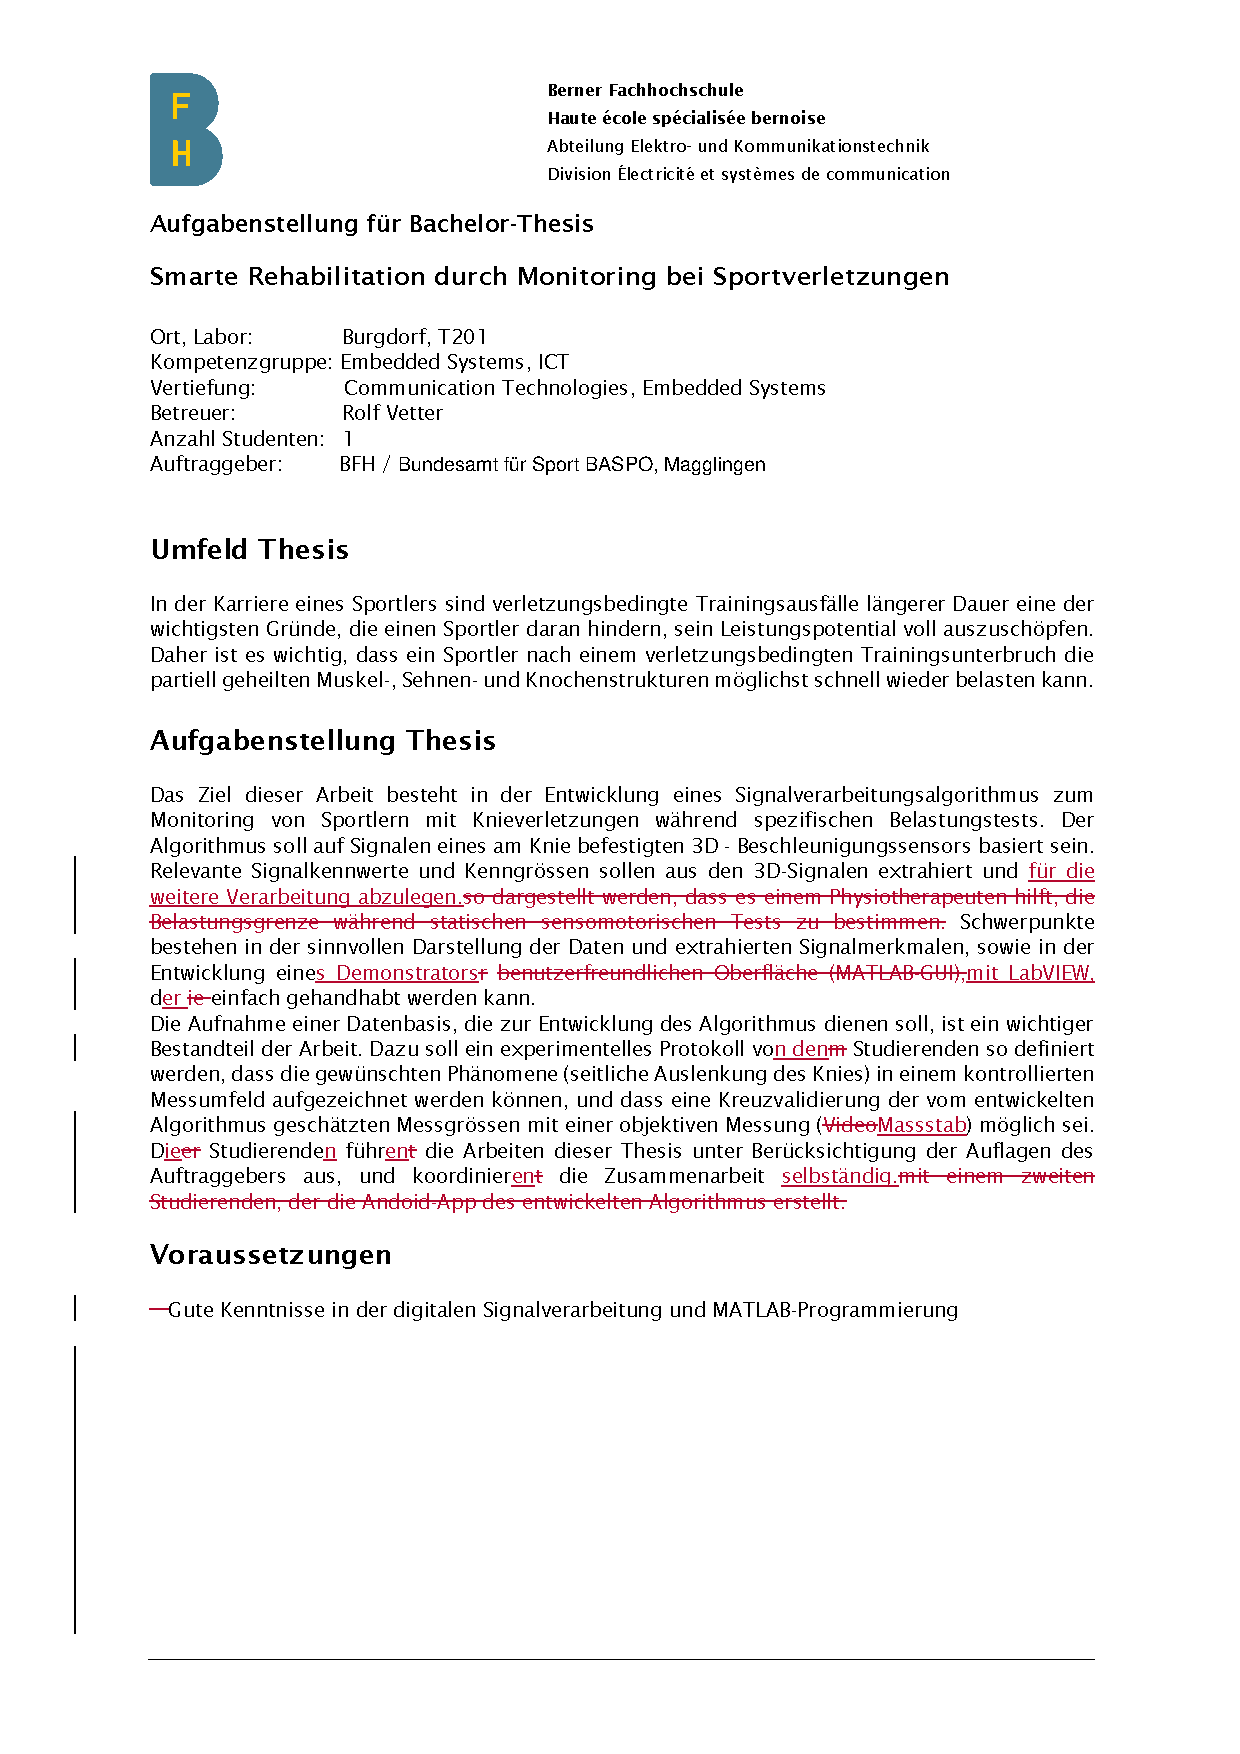
\includepdf[scale=0.8,pagecommand={},page=-,landscape=false]{appendix/aufgabenstellung/src/aufgabenstellung.pdf}

  
%
%Anhang C
%%%%%%%%%%%%%%%%%%%%%%%%%%%%%%%%%%%%%%%%%%%%%%%%%%%%%%%%%%%%%%%%%%%%%%%%%%%%%%%
% Titel:   Bericht - Messungen
% Autor:   gross10
% Datum:   20.06.2014
% Version: 0.0.1
%%%%%%%%%%%%%%%%%%%%%%%%%%%%%%%%%%%%%%%%%%%%%%%%%%%%%%%%%%%%%%%%%%%%%%%%%%%%%%%
%
%:::Change-Log:::
% Versionierung erfolgt auf folgende Gegebenheiten: -1. Release Versionen
%                                                   -2. Neue Kapitel
%                                                   -3. Fehlerkorrekturen
%
% 0.0.01      Erstellung der Datei
%%%%%%%%%%%%%%%%%%%%%%%%%%%%%%%%%%%%%%%%%%%%%%%%%%%%%%%%%%%%%%%%%%%%%%%%%%%%%%% 
\chapter{Messungen}\label{ch:messungen}\todo{Diagramm-Positionen}
	In diesem Kapitel sind alle Messergebnisse die w�hrend des Projekts aufgef�hrt. Die Gliederung folgt dabei der Reihenfolge der Durchf�hrung. 
    %
    \section{Konzept}\label{s:anhang_konzept_messung}
    	Messungen w�hrend der Konzeptphase.
    	%
    	\subsection{Translation}\label{ss:anhang_konzept_messung_translation}
    		\subsubsection*{x-Position}
    			\image{appendix/messung/image/mittel_5_X}{scale=0.6}{htbp}[x-Position Translation langsam][img:x_tran_langsam]
				%
				\image{appendix/messung/image/schnell_5_X}{scale=0.6}{htbp}[x-Position Translation schnell][img:x_tran_schnell]
			\subsubsection*{y-Position}
				\image{appendix/messung/image/mittel_5_Y}{scale=0.6}{htbp}[y-Position Translation langsam][img:y_tran_langsam]
				%
				\image{appendix/messung/image/schnell_5_Y}{scale=0.6}{htbp}[y-Position Translation schnell][img:y_tran_schnell]
			\subsubsection*{z-Position}
				\image{appendix/messung/image/mittel_5_Z}{scale=0.6}{htbp}[z-Position Translation langsam][img:z_tran_langsam]
				%
				\image{appendix/messung/image/schnell_5_Z}{scale=0.6}{htbp}[z-Position Translation schnell][img:z_tran_schnell]
		%
		\subsection{Translation und Rotation}\label{ss:anhang_konzept_messung_translation_rotation}
			%
			\subsubsection*{Auslenkung 1}
				\image{appendix/messung/image/auslenkung_1}{scale=0.6}{htbp}[Auslenkung 1][img:auslenkung_1]
			%
			\subsubsection*{Auslenkung 1}
				\image{appendix/messung/image/auslenkung_2}{scale=0.6}{htbp}[Auslenkung 2][img:auslenkung_2]
			%			
			\subsubsection*{Auslenkung 1}
				\image{appendix/messung/image/auslenkung_3}{scale=0.6}{htbp}[Auslenkung 3 langsam][img:auslenkung_2]
		
		   		
    	
    %
    \section{Implementation}\label{s:anhang_implementation_messung}
  
%
%Anhang D
%%%%%%%%%%%%%%%%%%%%%%%%%%%%%%%%%%%%%%%%%%%%%%%%%%%%%%%%%%%%%%%%%%%%%%%%%%%%%%%
% Titel:   Bericht - Pflichtenheft
% Autor:   gross10
% Datum:   13.12.2013
% Version: 0.0.1
%%%%%%%%%%%%%%%%%%%%%%%%%%%%%%%%%%%%%%%%%%%%%%%%%%%%%%%%%%%%%%%%%%%%%%%%%%%%%%%
%
%:::Change-Log:::
% Versionierung erfolgt auf folgende Gegebenheiten: -1. Release Versionen
%                                                   -2. Neue Kapitel
%                                                   -3. Fehlerkorrekturen
%
% 0.0.01      Erstellung der Datei
%%%%%%%%%%%%%%%%%%%%%%%%%%%%%%%%%%%%%%%%%%%%%%%%%%%%%%%%%%%%%%%%%%%%%%%%%%%%%%% 
\chapter{Auslesen DAQ-Karte mit MATLAB}\label{ch:daqauslesen}
\gls{g:matlab} bietet zum direkten Auslesen von Daten eine Data Acquisition Toolbox an. In dieser k�nnen angeschlossene \acrshort{ac:daq}-Karten in einer sogenannten Session direkt in \gls{g:matlab} beispielsweise mittels USB ausgelesen werden. Auch k�nnen Daten/Signale, welche in \gls{g:matlab} generiert wurden �ber Ausg�nge der Karte ausgegeben werden.\par 
Zum Auslesen eines Beschleunigungssensors wurde ein kurzes \gls{g:matlab}-Skript geschrieben. Dieses Skript sollte auch zuk�nftigen Arbeiten eine schnelle und einfache Verwendung der Beschleunigungssensoren erm�glichen.\par
\begin{lstlisting}[style=Matlab,caption={DAQ\_Auslesen.m},label={list:daqauslesen}]
%**************************************************************************
%   Smart Rehabilitation Thesis 2014 
%      
%   Skript zum initialisieren und auslesen des ICP-Beschleunigungssensors
%   603C01 von IMI Sensors mit der NI USB-4431 DAQ-Karte
%   
%   Reto Zurschmiede, Juni 2014
%**************************************************************************

clear all
close all
clc

% Laden des verwendeten Devices 
devices = daq.getDevices

% Port einstellen
devices(1)

% Session f�r NI Karte erstellen
s = daq.createSession('ni');

% Analogeingang hinzuf�gen
[ai0, ind0] = s.addAnalogInputChannel(devices.ID,'ai0','Accelerometer');

% Sensor initialisieren
s.Channels(ind0).Sensitivity = 100e-3;  % Sensitivit�t des Sensors [V/g]
ai0.Coupling = 'AC';                    % DC-Bias auskoppeln
ai0.ExcitationSource = 'Internal';      % Speisung des Sensors
ai0.ExcitationCurrent = 2e-3;           % Konstant Strom [A] 

% Abtastfrequenz einstellen [Hz]
s.Rate = 20e3;

% Aufzeichnungsdauer einstellen [s]
s.DurationInSeconds = 5;

% Daten auslesen
[data, time] = s.startForeground;

% Daten darstellen
figure 
plot(time,data)
xlabel('Time [s]')
ylabel('Acceleration [g]')
\end{lstlisting}
%
%Datenaufnahme mit ICP-Beschleunigungssensoren
\section*{Datenaufnahme mit ICP-Beschleunigungssensoren}
Um bei der Konzeptentwicklung Daten zum �berpr�fen des Algorithmus zu haben, erhielten wir von Rolf Vetter \gls{ac:icp}-Beschleunigungssensoren von IMI Sensors. Mit einer \gls{ac:daq}-Karte von \gls{ac:ni}, der \gls{ac:ni} USB-4431, wurden die Beschleunigungssensoren direkt mittels MATLAB ausgelesen. Somit sind die Daten direkt in MATLAB zur Weiterverarbeitung abgelegt. Es hat sich jedoch schnell herausgestellt, dass die Sensoren f�r unsere Anwendung nicht geeignet sind. Der Frequenzbereich des Sensors ist im Datenblatt in \vref{ch:indusriesensor} ersichtlich. Dort zu sehen ist, dass der Sensor einen Frequenzbereich von \unit[0.5]{Hz} bis \unit[10]{kHz} hat. Somit wird die f�r uns notwendige Gravitationsbeschleunigung, die einem DC-Anteil im Signal entspricht, nicht aufgenommen. Diese Sensoren k�nnen nur f�r dynamische Anwendungen verwendet werden wie Beispielsweise einer Ersch�tterungsmessung.


%
%Anhang E
%%%%%%%%%%%%%%%%%%%%%%%%%%%%%%%%%%%%%%%%%%%%%%%%%%%%%%%%%%%%%%%%%%%%%%%%%%%%%%%%
% Titel:   Bericht - Pflichtenheft
% Autor:   gross10
% Datum:   13.12.2013
% Version: 0.0.1
%%%%%%%%%%%%%%%%%%%%%%%%%%%%%%%%%%%%%%%%%%%%%%%%%%%%%%%%%%%%%%%%%%%%%%%%%%%%%%%
%
%:::Change-Log:::
% Versionierung erfolgt auf folgende Gegebenheiten: -1. Release Versionen
%                                                   -2. Neue Kapitel
%                                                   -3. Fehlerkorrekturen
%
% 0.0.01      Erstellung der Datei
%%%%%%%%%%%%%%%%%%%%%%%%%%%%%%%%%%%%%%%%%%%%%%%%%%%%%%%%%%%%%%%%%%%%%%%%%%%%%%% 
%\chapter{Industrie ICP Beschleunigungssensor}\label{ch:indusriesensor}
%    Datenblatt des \acrshort{ac:icp} Beschleunigungssensors 603C01 von IMI Sensors.
%    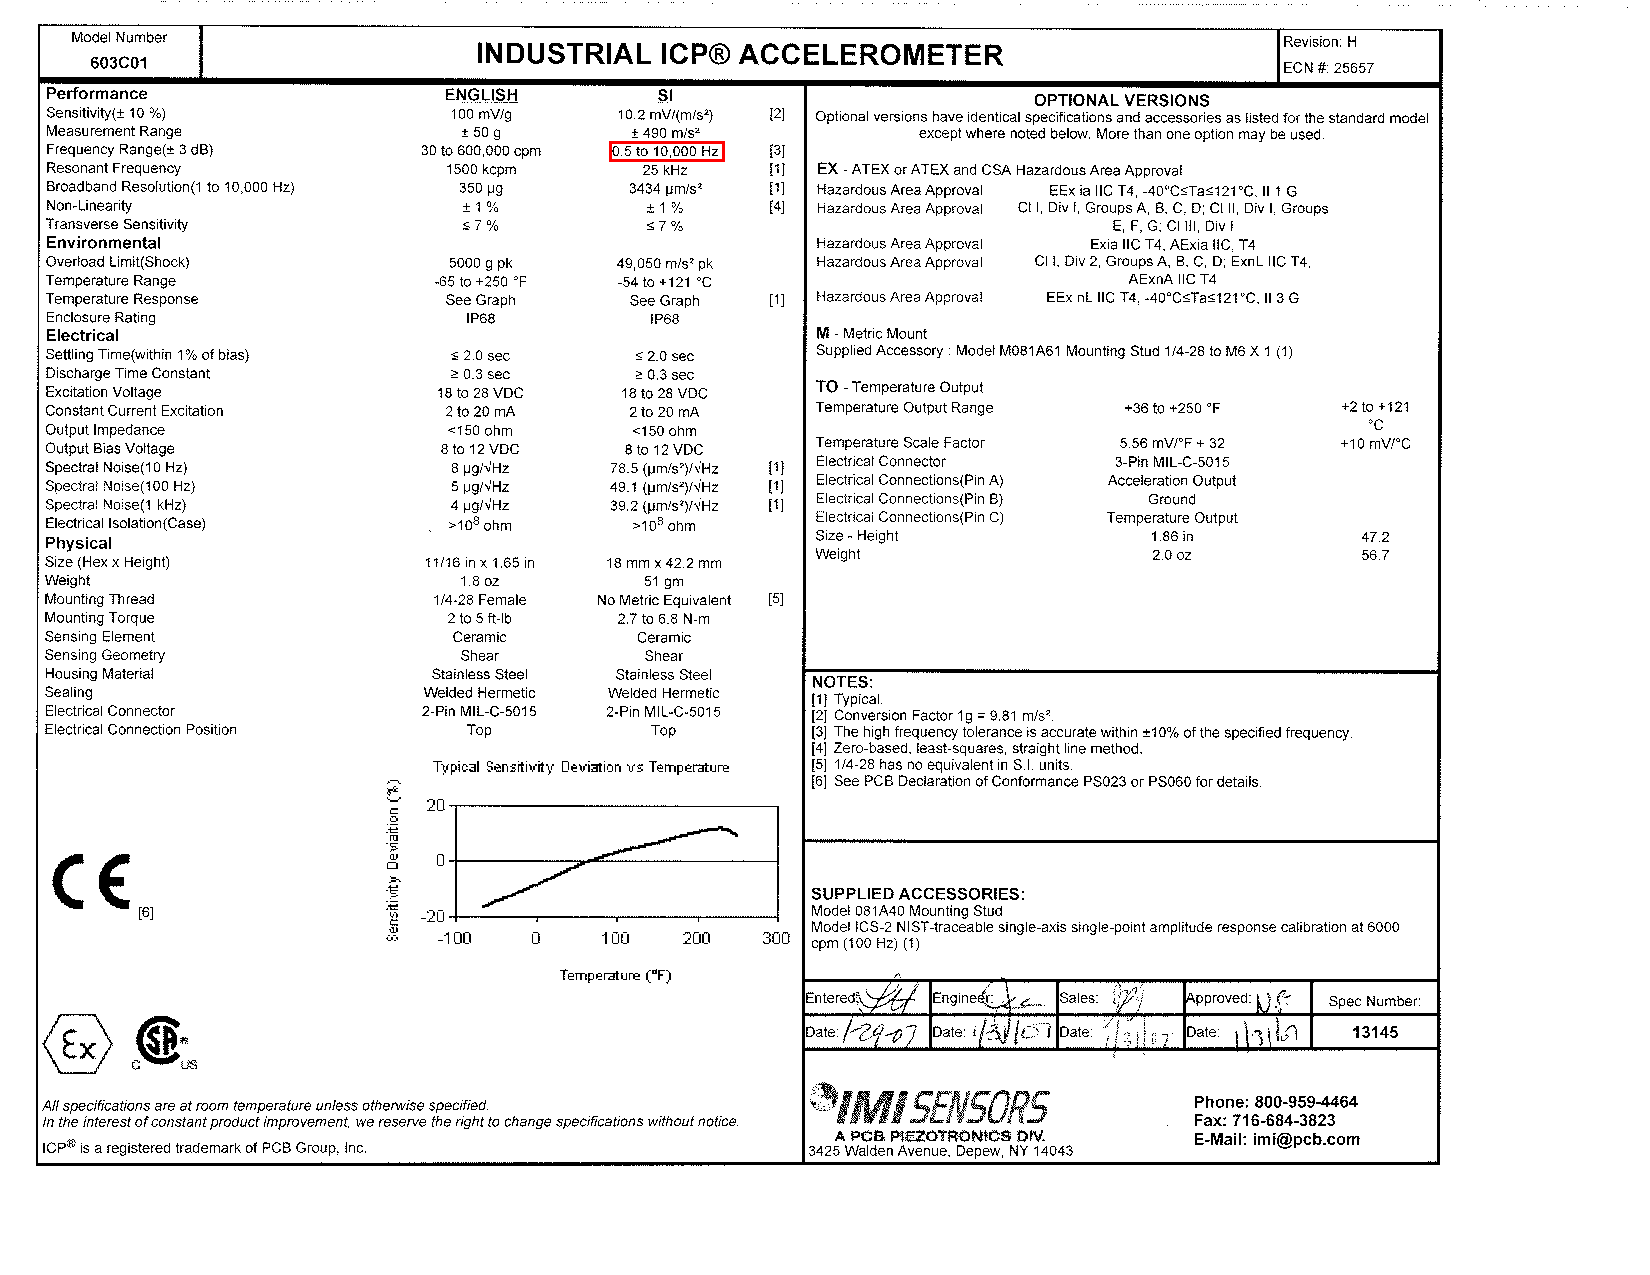
\includepdf[scale=0.7,pagecommand={},page=-,landscape=true]{appendix/datasheet/src/603C01_H.pdf}
%%
%\chapter{NI USB-4431}\label{ch:niusb4431}
%	Datenblatt der \gls{ac:daq}-Karte \acrshort{ac:ni} USB-4431.
%	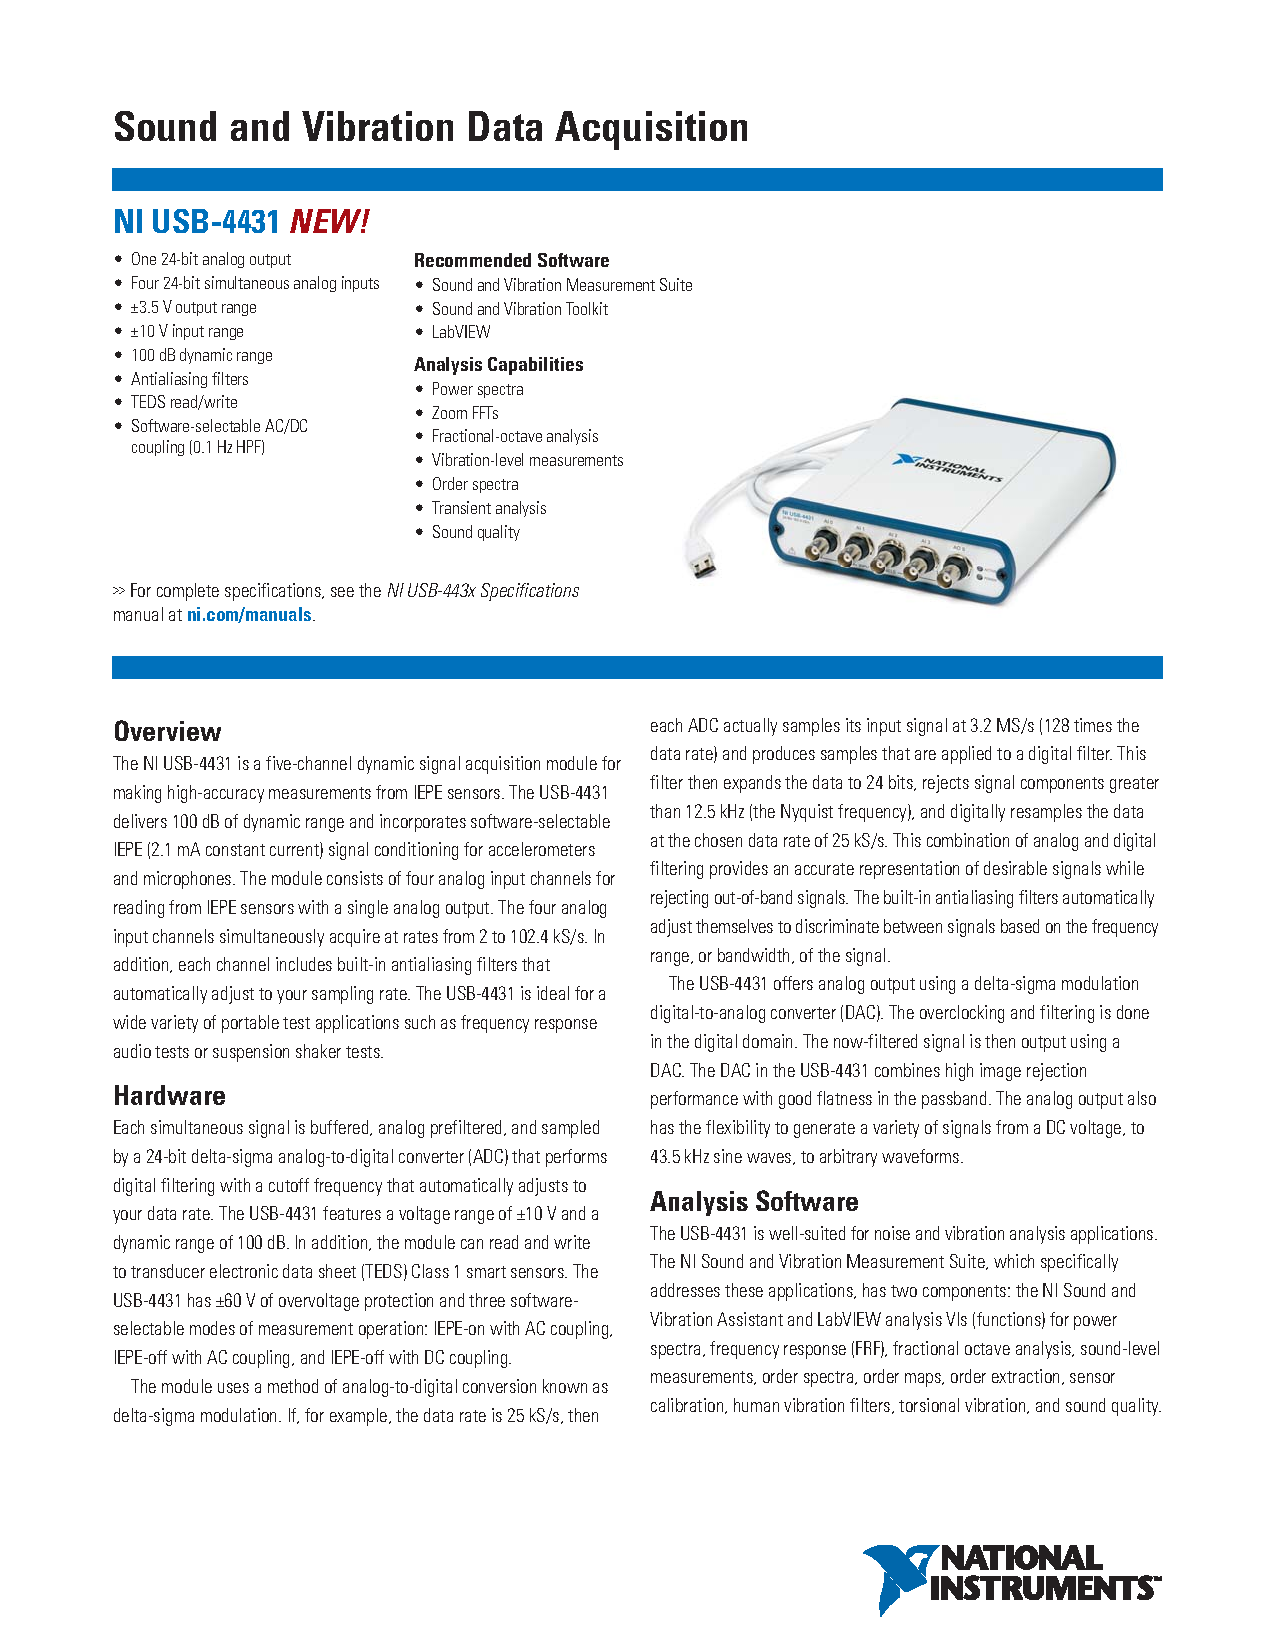
\includepdf[scale=0.7,pagecommand={},page=-,landscape=false]{appendix/datasheet/src/cat_usb4431.pdf}
%	
\chapter{NI myRIO}\label{ch:datasheet_myrio}
	Datenblatt des \gls{ac:daq}\gls{g:myrio} Developmentboard.
	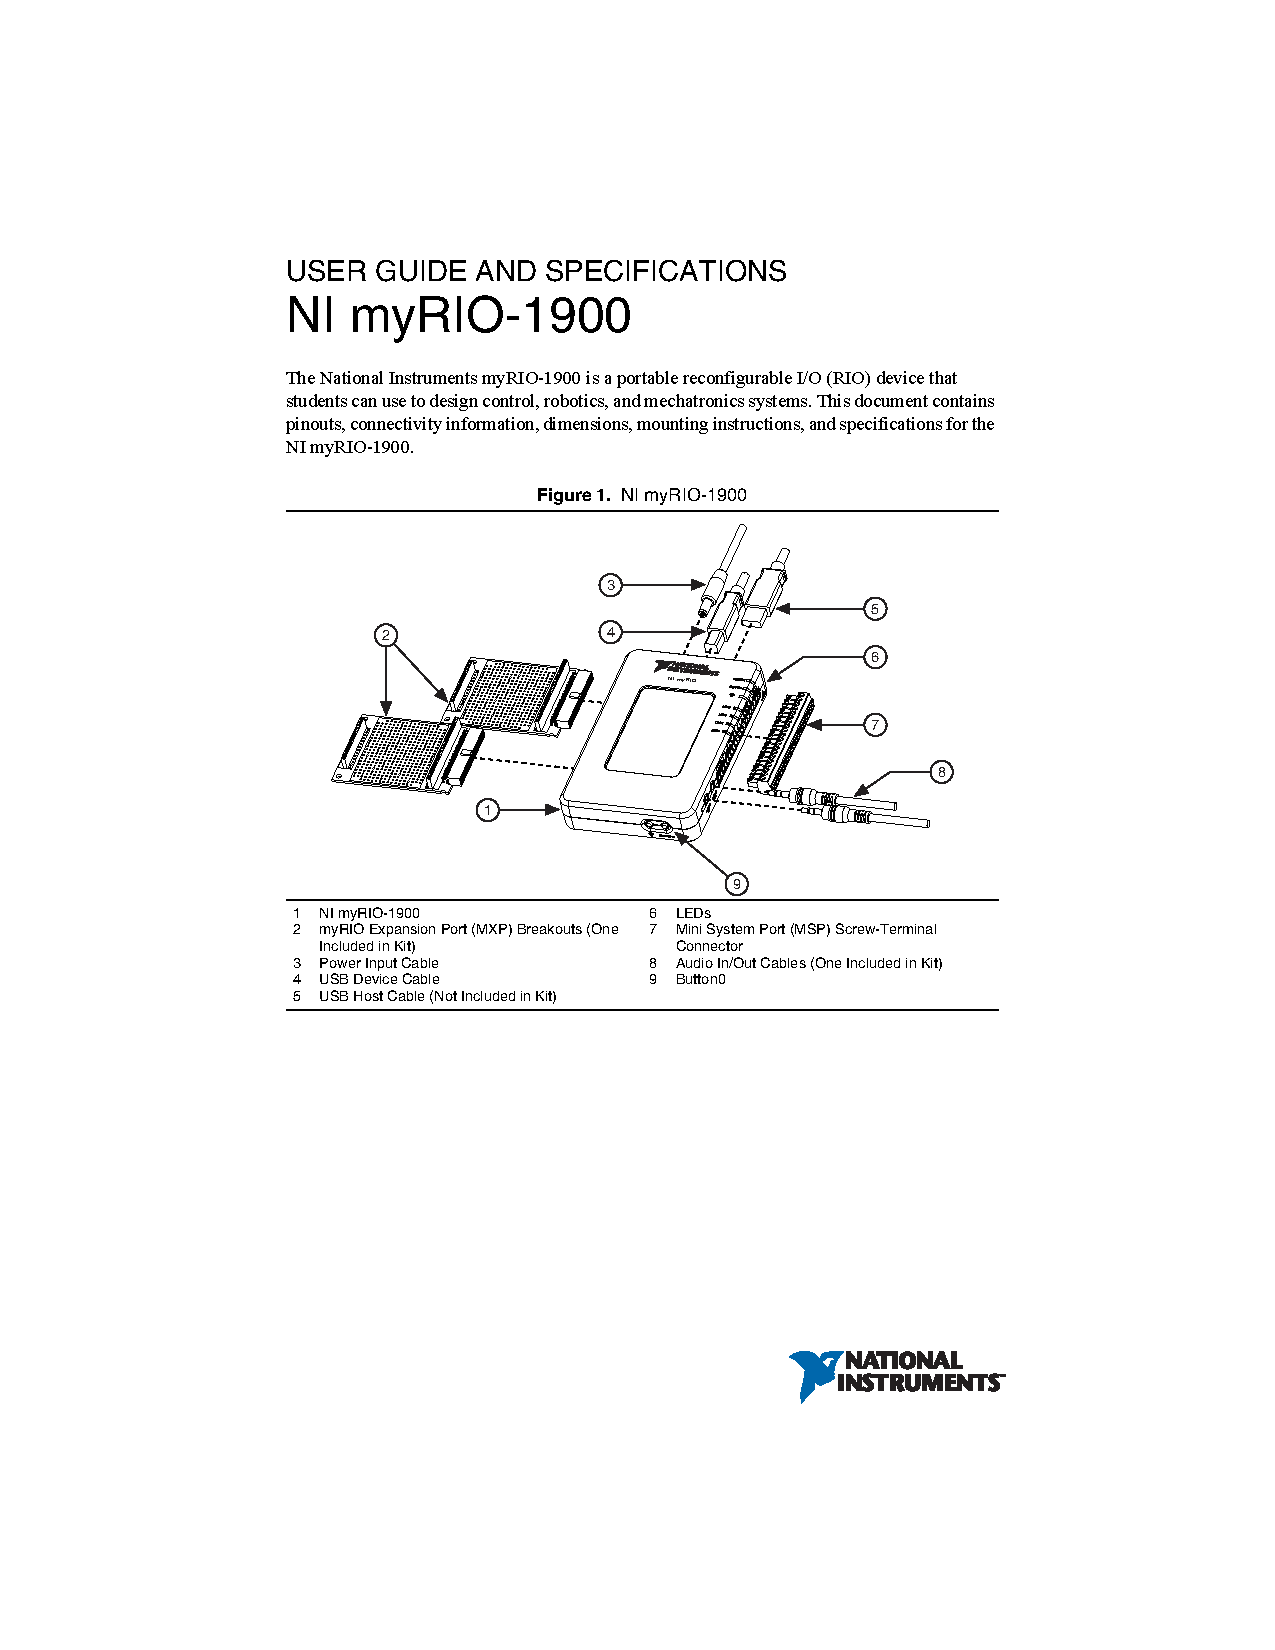
\includepdf[scale=0.7,pagecommand={},page=-,landscape=false]{appendix/datasheet/src/myRIO_1900.pdf}
  
%
%Anhang F
%%%%%%%%%%%%%%%%%%%%%%%%%%%%%%%%%%%%%%%%%%%%%%%%%%%%%%%%%%%%%%%%%%%%%%%%%%%%%%%
% Titel:   Bericht - CD
% Autor:   gross10
% Datum:   19.06.2014
% Version: 0.0.1
%%%%%%%%%%%%%%%%%%%%%%%%%%%%%%%%%%%%%%%%%%%%%%%%%%%%%%%%%%%%%%%%%%%%%%%%%%%%%%%
%
%:::Change-Log:::
% Versionierung erfolgt auf folgende Gegebenheiten: -1. Release Versionen
%                                                   -2. Neue Kapitel
%                                                   -3. Fehlerkorrekturen
%
% 0.0.01      Erstellung der Datei
%%%%%%%%%%%%%%%%%%%%%%%%%%%%%%%%%%%%%%%%%%%%%%%%%%%%%%%%%%%%%%%%%%%%%%%%%%%%%%% 
\chapter{CD}\label{ch:cd}
	Aus �kologischen und �konomischen Gr�nden wird ein grosser Teil des Anhangs in Form einer CD-ROM dieser Dokumentation beigelegt. Die Dateistruktur entspricht dabei der Gliederung dieses Kapitels.
    %
    \section{LabVIEW}
    	Alle ben�tigten \gls{g:labview}-Projekte:
    	%
    	\begin{itemize}
	    	\item \textbf{Konzept}: \texttt{concept\_reametric}
	    	\item \textbf{Implementierung}: \texttt{reametric}
    	\end{itemize}
    %
    \section{MATLAB}
  

%

%
%
\end{document}
